\tolerance=10000

\documentclass[12pt]{report}
\usepackage{graphicx}

%This package is built on the LaTeX2e report class, so any other packages which are
%also compatible with it can also be used in combination with it.  ODUthesis should
%be in the directory in which you are working, or in one of the standard input directories
%for the TeX installation on your system.

\usepackage{ODUthesis}
\usepackage{amsmath}
\usepackage{float}
\usepackage{gensymb}
\usepackage{url}
\usepackage{feynmp-auto}
\usepackage{hyperref}
\usepackage{amssymb}

%This package causes the first line of a section to be indented as required by the dissertation guide.

\usepackage{indentfirst}
\usepackage{booktabs}

%%%%%Other LaTeX2e packages such as the AMS fonts and graphics packages can be included here.

%This style follows conventions used in Physical Review C. The names of figures, tables and captions can
%be changed by using the commands below with appropriate changes. For example, "FIG." could be replaced by
%"Fig." or "Figure" to change the labeling of figure captions.

%\renewcommand{\figurename}{FIG.}
%\renewcommand{\tablename}{TABLE}
%\renewcommand{\bibname}{BIBLIOGRAPHY}

\usepackage{chngcntr}
\counterwithin{figure}{section}

\counterwithin{equation}{section}

\begin{document}

\title{Searching for Heavy Photons with Detached Vertices in the Heavy Photon Search Experiment}

\author{Holly Szumila-Vance}
\principaladviser{Lawrence Weinstein}
\member{John Adam}
\member{Wally Van Orden}
\member{Stepan Stepanyan}  %This command produces a signature line for the specified member on the
\member{Lepsha Vuskovic}  %title page. Use on instance of this command for each member of the
                   %committee other than the advisor up to a total of 5 members.

\degrees{B.S. May 2008, Embry-Riddle Aeronautical University \\ B.S. May 2009, Embry-Riddle Aeronautical University \\ M.S. May 2014, Old Dominion University}


\dept{Physics}          %for example \dept{physics}

\submitdate{June 2017}

%\phdfalse          %produces language on title page for Masters Thesis. Otherwise the default
                    %is for a Ph.D. dissertation.

%\copyrightfalse    %suppresses copyright notice

%\figurespagefalse  %suppresses List of Figures

%\tablespagefalse   %suppresses List of Tables

\vita{The text of the Vita goes here.}


\abstract{The Heavy Photon Search (HPS) experiment is an experiment at Jefferson Lab that searches for a hypothetical massive particle called the heavy photon which could mediate a dark electromagnetic-type force. If heavy photons kinetically mix with Standard Model photons, they may be radiated by electrons scattering from a heavy nucleus and then decay to $e^+e^-$ pairs. HPS uniquely searches for heavy photons that either decay at the target or a measurable distance after. The experiment utilizes a silicon vertex tracker  (SVT) for momentum and vertex reconstruction, together with an electromagnetic calorimeter for measuring particle energies and triggering events. The HPS experiment took its first data during the spring 2015 Engineering Run using a 1~GeV electron beam incident on a tungsten target and completed a second run in the spring 2016 Physics Run at a beam energy of 2.3 GeV. \\
\indent The focus of this dissertation discusses the displaced vertex search for heavy photons in the 2015 Engineering Run. This dissertation describes the theoretical motivation for looking for heavy photons and provides an overview of the HPS experimental design and performance. The performance details of the experiment are primarily derived from the 2015 Engineering Run with some discussion from the higher energy running in 2016. \\
\indent The displaced vertex analysis combines the results obtained from data taken with the SVT at its nominal position at $\pm$0.5~mm from the beam and data taken with the SVT slightly open at $\pm$1.5~mm from the beam. The final results are dominated by the events passing through the first tracking layer of the SVT but also include events that missed the first tracking layer. In total, the final data set has an integrated luminosity of 1529~nb$^{-1}$ of which 1166~nb$^{-1}$ was taken with the SVT at the nominal position at $\pm$0.5~mm from the beam. \\
\indent No limit is obtained from the displaced vertex search due to having not taken enough data. After un-blinding the data, the results from extensive studies on an additional background in the full data set are discussed. Improvements to the vertex reconstruction are expected to play a major part in the isolation of these backgrounds in the future of the experiment.}

\beforepreface

\prefacesection{Acknowledgments} 

    %text of Acknowledgments goes here
    %any other preface section is inserted similarly by the command
    %\prefacesection{Section Title}

\afterpreface

    %The text of the thesis/dissertation begins here. The basic organization is
    %in chapters, sections, subsections. 

\chapter{Introduction}
The heavy photon, also known as the $A^{\prime}$, is a theoretically motivated massive gauge boson that is associated with a predicted U(1) hidden symmetry, favorable to Beyond Standard Model theories. According to theory~\cite{holdom_two_1986}, a heavy photon kinetically mixes with the Standard Model photon through a loop-level effect generating an effective coupling to electric charge. The relative size of this coupling to electric charge, $\epsilon$, can range from $10^{-12}$ to $10^{-2}$ depending on the loop order of the mixing interaction and describes the coupling of the heavy photon to electric charge to be at a scale significantly smaller than that in standard electrodynamic theory. While the coupling strength of the interaction can be naturally generated from the loop interactions, the mass is somewhat less constrained. Theories of the heavy photon as a way to explain cosmological phenomena make them the simplest and possibly leading interaction between the Standard Model and the Dark Sector. The Dark Sector encompasses both dark matter and dark energy particles that do not interact other than gravitationally. If the heavy photon obtains its mass through the Higgs mechanism, the mass is favored to be in the range of MeV to GeV which is compatible with dark matter theories. In such a scenario, electrons could radiate heavy photons as they do ordinary photons but at a suppressed rate. These heavy photons will have measurable lifetimes before decaying to charged particle pairs. It is natural to describe the heavy photon parameter space in terms of its coupling, $\epsilon^2$, and mass, $m_{A'}$.\\
\begin{figure}[htb]
  \centering
      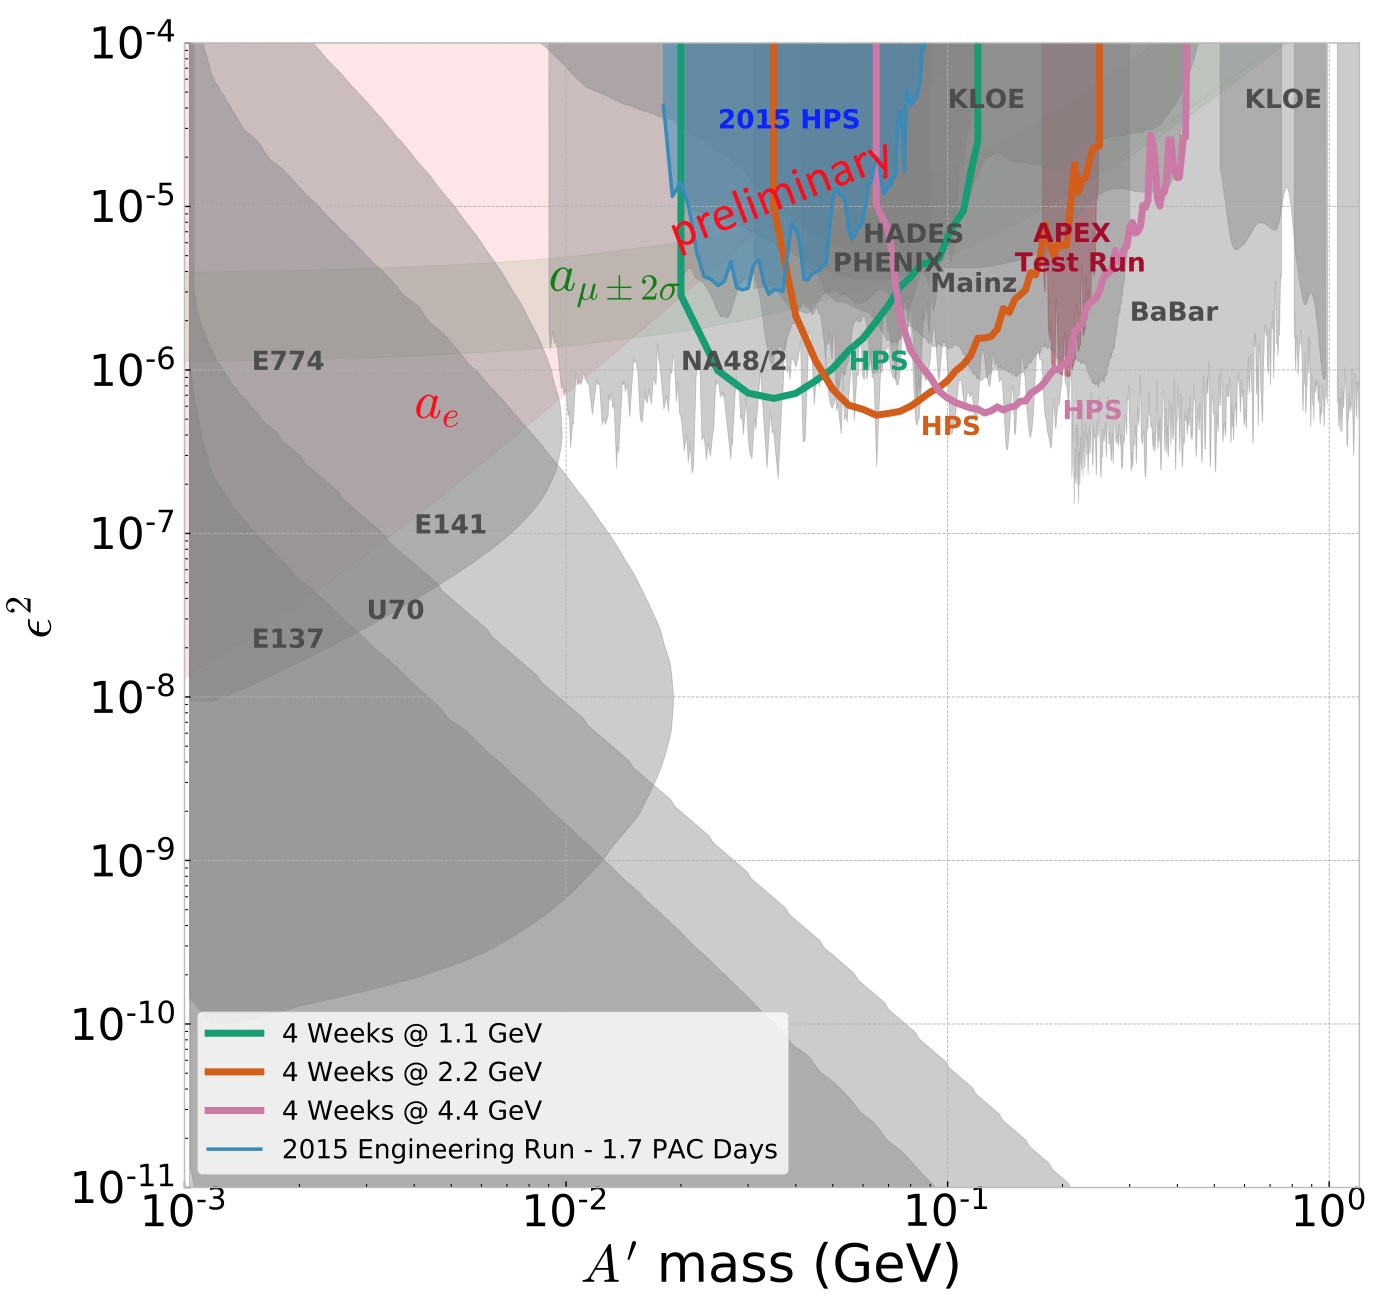
\includegraphics[width=0.7\textwidth]{pics/intro/reach_nominal.png}
  \caption[Reach for the HPS experiment]{The existing 90$\%$ confidence limits from other experiments looking for heavy photons in the relevant mass-coupling region is shown. The shaded blue region includes the preliminary bump hunt results from the 2015 engineering run. The vertex reach is not shown on this plot as no reach is found using the proposed HPS run configuration. The region labeled as $a_\mu$ indicates the favored parameter space for a visibly decaying heavy photon to explain the discrepancy between the calculated and measured muon anomalous magnetic moment. The experiments along the top of the plot with large coupling look for heavy photons that decay promptly at the target. The limits shown in grey along the left side of the plot with decreasing values of coupling look for heavy photons with displaced vertices in beam dump experiments.}
      \label{Figure:projectedReach}
\end{figure}
\indent The Heavy Photon Search (HPS) experiment is searching for heavy photons in the mass range of 20 to 1000~MeV/c$^2$ with prompt or displaced vertices with respect to the target interaction. HPS  generates heavy photons from an electron beam incident on a heavy target and measures the momentum and vertex position of $e^+e^-$ pairs produced from its decay. By reconstructing the invariant mass and the vertex position of the pairs, HPS can look for a small bump on a large background using a bump hunt for prompt decays. Uniquely, HPS is also able to look for heavy photons with smaller couplings (and longer lifetimes) characterized by displaced vertices by searching for a small signal on low background downstream of the target. The HPS reach attained from the 2015 engineering run from the bump hunt is shown in Figure~\ref{Figure:projReach} along with the existing limits from other experiments.\\
\indent The HPS experiment took place in Hall B at the Jefferson Laboratory National Accelerator Facility. The Continuous Electron Beam Accelerator Facility (CEBAF) at Jefferson Lab produces an electron beam that collides with the HPS target material in Hall B. The HPS detector measures the particles from this interaction and searches for the heavy photon signal. The HPS detector consists of a Silicon Vertex Tracker (SVT) and an Electromagnetic Calorimeter (ECal). The SVT measures particle trajectories and reconstructs the vertex position of the particle pair. The ECal triggers event readout in addition to measuring particle energy and pair coincidence timing. \\
\indent The ECal was commissioned during a short commissioning run in December 2014. The full experiment ran in the spring of 2015 commissioning the full beamline and both detectors. This run took 2.3~days of good data at approximately 50~nA with a beam energy of 1.056~GeV. HPS obtained a total of 1529~nb$^{-1}$ of good data. During the commissioning of the SVT, some data was taken with the SVT slightly open from its nominal position before moving the SVT in to its designed position at $\pm0.5$~mm from the beam. A second run in the spring of 2016 used a 200~nA electron beam at 2.3~GeV collecting a total of 5.7~days of data.  Future running at higher electron beam energy is planned for 2018 and beyond.\\
\indent In this dissertation, I describe the search for heavy photons with a displaced vertex using data from the 2015 engineering run. I will describe the experiment as a whole focusing on the areas in which I was most involved. I performed a blinded analysis using 10$\%$ of the data. In order to better understand and analyze the backgrounds in the vertex search, I conducted a further study of the backgrounds using the statistics of the fully unblinded dataset. I will discuss the backgrounds and reach from the Engineering Run.\\
\indent In addition to the full vertex analysis, I contributed significantly to the assembly, characterization and commissioning of the ECal for all experimental running. I wrote the clustering algorithm based on that used by the CLAS experiment Inner Calorimeter (IC) and improved simulations of the ECal detector response. I also calibrated the ECal in both energy and time for both experimental runs. 

%%%%%%%%%%%%%%%%%%%%%%%%%%%%%%%%%%%%%%%%%
\chapter{Motivation} 
The Standard Model (SM) is the most successful theory for describing elementary particles and their interactions via the electromagnetic, strong, and weak forces in terms of gauge theory interactions. The existence of an additional U(1) hidden symmetry is not forbidden by the SM. The heavy photon is the proposed gauge boson for the dark electromagnetic force that would arise from a U(1) broken symmetry. If such an interaction exists, then the SM photon and heavy photon would mix, thus inducing a coupling between the heavy photon and electric charge equal to $\epsilon e$~\cite{holdom_two_1986}. This coupling is significant because electrons could radiate heavy photons similar to radiating SM photons, although at rates decreased by $\epsilon^2$. The primary goal of HPS and many similar experiments is to experimentally detect the heavy photon through this production mechanism. The heavy photon is additionally referred to as the $A^{\prime}$, dark photon, or $U-$boson.

\section{Theory of heavy photons}
The postulation for the heavy photon rests of an exploitation of allowable symmetries from the Standard Model. An additional U(1) symmetry in nature could interact with the SM through the mechanism of kinetic mixing~\cite{Holdom0}. In this model, the charge of SM particles would be shifted by some amount $\epsilon$ that is related to the strength of the new gauge boson (heavy photon or A$^{\prime}$ coupling to the SM charge. Kinetic mixing generates a coupling, $\epsilon$ through loop interactions as shown in Figure~\ref{fig:loop}. 

\begin{figure}[H]
    \begin{center}
        \begin{fmffile}{loop}
            \begin{fmfgraph*}(150,150)
                \fmfstraight 
                \fmfleft{i1}
                \fmfright{o1}
                \fmflabel{$\gamma$}{i1}
                \fmflabel{$A'$}{o1}
                \fmf{photon,tension=1}{i1,v1}
                \fmf{photon,tension=1}{v2,o1}
                \fmf{fermion,left,label=$\chi$}{v2,v1}
                \fmf{fermion,left,label=$\chi^{\prime}$}{v1,v2}
            \end{fmfgraph*}
        \end{fmffile}
    \end{center}
    \caption[Kinetic mixing of the SM photon with a heavy photon]{Kinetic mixing of the SM photon with a heavy photon is shown at the one-loop level. $chi$ can be any massive particle that is charged under both the A$^{\prime}$ and SM U(1) interactions.}
    \label{fig:loop}
\end{figure}

In the simplest scenario, there is one particle $\chi$ that is charged under both the U(1) and new U(1)$^{\prime}$. This single loop level interaction can generate the $\epsilon$ coupling to be in the range of $10^{-2}$ to $10^{-4}$. In Grand Unified Theory (GUT), symmetries forbid one-loop interactions and favor two-loop interactions generating an $\epsilon$ in the range of $10^{-3}$ to $10^{-5}$.~\cite{DarkSectors2016} If both U(1)s are in unified groups, higher loop interactions generating even smaller couplings are possible. The gauge part of the SM Lagrangian is modified to include this interaction as shown in Equation~\eqref{eq:lagrangian} 
\begin{equation}
	\label{eq:lagrangian}
\mathcal{L}_{gauge} = -\dfrac{1}{4}F^{\mu\nu}F_{\mu\nu}-\dfrac{1}{4}
F^{\prime\mu\nu}F^{\prime}_{\mu\nu}-\dfrac{1}{4}\epsilon F^{\mu\nu}F^{\prime}_{\mu\nu}
\end{equation}

In Equation~\eqref{eq:lagrangian}, $F_{\mu\nu}$ is the electromagnetic field strength tensor defined in terms of the gradient of the potential as $\partial_{\mu}A_{\nu}-\partial_{\nu}A_{\mu}$. $F^{\prime}_{\mu\nu}$ corresponds to the field strength of the heavy photon and $\epsilon$ is the coupling. The third term of the Lagrangian is the kinetic mixing operator. The SM photon field can be re-defined as $A_{\mu}\rightarrow A_{\mu}+\epsilon A^{\prime}_{\mu}$ to remove the kinetic mixing operator. This generates a coupling to electric charge of order $\epsilon$ seen in the interaction between the heavy photon and SM as $\epsilon e A^{\prime}_{\mu}J^{\mu}_{EM}$ where $J^{\mu}_{EM}$ is the electromagnetic current.~\cite{toro} Particles that are charged only under the A$^{\prime}$ would not acquire this fractional charge and would remain undetectable in this model. \\
\indent The mass of the heavy photon is somewhat less constrained by theory. The MeV to GeV mass scale is interesting to explore because it has been generally overlooked in previous experimentation and is consistent with dark matter theories that attempt to explain several astrophysical phenomena. 



\section{Implications of a heavy photon}
Update this section with Philip's talk in May
\subsection{Dark matter}
Discuss excess of gamma rays at Galactic Center and focus on dark matter models in the low mass regime. 
\subsection{Constraints}
Discuss g-2, AMS-02, CMB 



\section{Searching for heavy photons}
The final states to which the heavy photon can decay into is related to the model of the dark sector, and corresponding dark matter mass $m_{\chi}$, one is considering. For a heavy photon that is heavier than $m_{\chi}$, then the heavy photon may decay into completely invisible states or a mixture of invisible states and SM states. For the scenario that the heavy photon decays to completely invisible states, the experiment will perform a missing mass or missing momentum measurement in order to identify the heavy photon signal. Here, we focus solely on the scenario of a heavy photon that decays visibly to SM particles (this also implies that the heavy photon is lighter than the dark matter mass). Due to the mechanism of kinetic mixing, the production of the heavy photon is similar to that of a photon radiating from an electron although at a suppressed rate proportional to the coupling $\epsilon^2$. 

\subsection{Decay signature}
The branching ratio of the heavy photon is derived from the ratios of different final state measurements of $e+e-\rightarrow$ hadrons at various center-of-mass energies~\cite{liu_signals_2015}. In the mass regime that HPS explores, the heavy photon can be expected to primarily decay to $e+e-$ pairs as shown in Figure~\ref{Figure:br}. 

\begin{figure}[H]
  \centering
      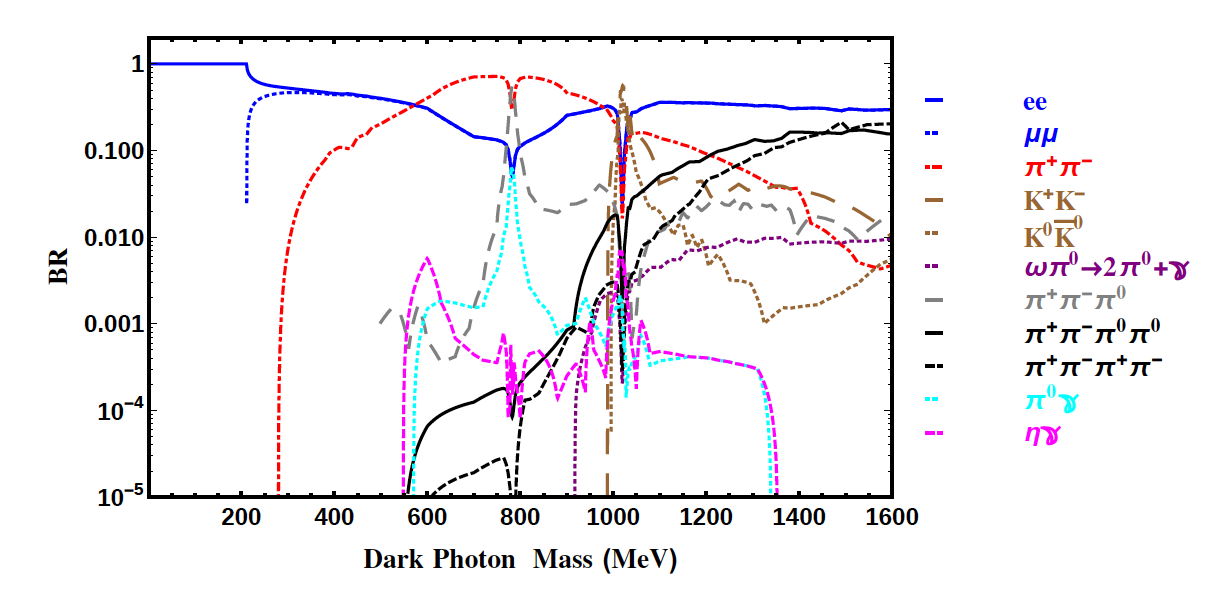
\includegraphics[width=0.9\textwidth]{pics/motivation/branchingRatio.png}
  \caption[The branching ratios for heavy photon decays]{The branching ratios for heavy photons of various masses.~\cite{liu_signals_2015}}
  \label{Figure:br}
\end{figure}

HPS searches for heavy photons of masses 20 to 100~MeV/c$^2$. As shown in Figure~\ref{Figure:br}, at heavy photon masses above 200~MeV/c$^2$, the branching ratio for decays to $e+e-$ begins to decrease sharply and the turn on for decays to $\mu+\mu-$ becomes significant. \\
\indent Assuming that the heavy photon only decays to SM final states, the proper lifetime of the A$^{\prime}$ neglecting phase space corrections is described by Equation~\eqref{eq:propLife} where $N_{eff}$ is the number of available decay states ($=1$ at $m_{A^{\prime}}<2m_{\mu}$).~\cite{toro} 

\begin{eqnarray}
	\label{eq:propLife}
	c\tau &=& \dfrac{1}{\Gamma}\simeq \dfrac{3}{N_{eff}m_{A^{\prime}}\alpha\epsilon^2}\\
	&\simeq & \dfrac{0.8\textsf{ cm}}{N_{eff}}\Big({\dfrac{10^{-4}}{\epsilon}}\Big)^2\Big(\dfrac{100\textsf{ MeV}}{m_{A^{\prime}}}\Big)\\
\end{eqnarray}

As shown in Equation~\eqref{eq:propLife}, the lifetime is inversely related to the coupling $\epsilon^2$. For small couplings, the heavy photon will travel a measurable distance after production before decaying. The decay length is described by Equation~\eqref{eq:decayL}.

\begin{eqnarray}
	\label{eq:decayL}
	l_0 &\equiv &\gamma c \tau \\
	&\simeq & \dfrac{0.8\textsf{ cm}}{N_{eff}}\Big(\dfrac{E_{beam}}{10\textsf{ GeV}}\Big)\Big({\dfrac{10^{-4}}{\epsilon}}\Big)^2\Big(\dfrac{100\textsf{ MeV}}{m_{A^{\prime}}}\Big)^2\\
\end{eqnarray}

In Equation~\eqref{eq:decayL}, $E_{beam}$ refers to the incident beam energy of the electron. The rate of A$^{\prime}$ production is controlled by $\alpha^3\epsilon^2/m_{A^{\prime}}^2$ and is suppressed relative to ordinary bremsstrahlung by a factor of $\epsilon^2m_{e-}^2/m_{A^{\prime}}^2$. The ratio of the fully differential production cross sections for the heavy photon relative to the production of a virtual photon are described in Equation~\eqref{eq:production}.

\begin{equation}
	\label{eq:production}
	\dfrac{d\sigma(e-Z(A^{\prime}Z\rightarrow l+l-))}{d\sigma(e-Z(\gamma^{\ast}Z\rightarrow l+l-))} = \Big(\dfrac{3\pi\epsilon^2}{2N_{eff}\alpha}\Big) \Big(\dfrac{m_{A^{\prime}}}{\delta m_{A^{\prime}}}\Big)
\end{equation}

In Equation~\eqref{eq:production}, this ratio represents the maximum signal to background that can be achieved in an experiment. The heavy photon is produced at very forward, small angles and carries nearly all of the beam energy. \\

\subsection{Methods of production}
Heavy photons can be produced experimentally in fixed-target experiments and collider experiments. Fixed-target experiments are complementary to collider experiments in that they can generally access smaller coupling due to the high luminosity while collider experiments can probe higher heavy photon masses due to the higher center of mass energy attainable. In electron fixed-target experiments, the heavy photon is generated through a bremsstrahlung-like process and is detected from the final state particles. Proton fixed-target experiments look for the signal in the decay products of various meson decay channels produced from the beam interaction at the target. Looking for heavy photons produced in meson decays such as Dalitz decays ($\pi^0, \eta, \eta^{\prime}\rightarrow \gamma A^{\prime}$), ($K\rightarrow\pi A^{\prime} $, $\phi\rightarrow\eta A^{\prime}$, and $D^{\ast}\rightarrow D^{0}A^{\prime}$) are another production mechanism that has been used at both colliders and fixed target-type experiments. Drell-Yan ($q\bar{q}\rightarrow A^{\prime}$) experiments are more common at proton fixed target and hadron collider experiments. Both $e+e-$ colliders and hadron colliders search from heavy photons in the decay channels listed above and are particularly well-suited to search for heavy photons that decay invisibly due to the ability to precisely reconstruct the initial state. 

\subsection{Methods of detection}

The strategies for searching for heavy photons are typically a bump hunt on the visible final state particles, a bump hunt in the missing mass spectrum (assumes that the heavy photon does not decay visibly), or a detached vertex search for heavy photons with small couplings. \\
\indent Electron fixed target experiments produce heavy photons through bremsstrahlung-like processes with the electron beam incident on a heavy target. Heavy photons are produced in a very forward direction requiring high resolution spectrometers or detectors close to the beam. Previous limits set by this type of experiment include the A1 experiment that uses the Microtron beam at Mainz and the A1 high resolution spectrometer to reconstruct $e+e-$ pair~\cite{beranek_theoretical_2013}. The A1 significantly ruled out parameter space where the heavy photon was a possible explanation to resolve the muon $g-2$ anomaly. The APEX experiment at Jefferson Lab ran a test run experiment that produced electron bremsstrahlung in Hall A and used the high resolution spectrometers to measure the $e+e-$ particles~\cite{abrahamyan_search_2011}. APEX performed a bump hunt on the final state particles in the mass range 65-600~MeV and will likely take data again in 2018. DarkLight is another Jefferson Lab experiment that places a windowless gas target in the Low Energy Recirculator Facility using a 100~MeV beam to search for heavy photons with low masses. DarkLight will perform a bump hunt search in the $e+e-$ mass spectrum and may have some ability to search for invisible decays by using a silicon layer to detect proton recoils~\cite{alewski_darklight_2014}.\\
\indent Proton fixed target experiments look for heavy photons in the decays of particles produced from beam interaction at the target. The NA48/2 experiment at the CERN SPS produced $K^{\pm}$ beams and searches for heavy photons from the $\pi^0$ decay produced from in the in-flight decay of the $K^{\pm}$~\cite{Batley_2015lha}. SHiP is future experiment at the CERN SPS that will use a 400~GeV proton beam and will look in both Drell Yan and meson decays for heavy photons. SHiP will be sensitive to long decay lengths (on the order of 10s of meters) and will cover a wide mass range in visible decay states up to 10~GeV masses. SHiP is expected to run sometime after 2026~\cite{ship_collaboration_facility_2015}.\\
\indent Beam dump experiments look for heavy photons with long decay lengths. The beam dump experiments E141 and E137 at SLAC, E774 at Fermilab, and one at Orsay were originally run to look for MeV-mass axion-type particles from electron beam dumps~\cite{alexander_dark_2016}. The U70 beam dump looked for heavy photons downstream from a proton beam on a fixed target. SeaQuest at Fermilab looks for muon pairs produced downstream from the 120~GeV proton beam on a fixed target. It is speculated that by analyzing previous data taken (E906/SeaQuest), a 95$\%$ confidence limit on heavy photon masses in the range of 215-5600~MeV is possible. SeaQuest is currently establishing upgrades for improved future running~\cite{gardner_new_2016}.
\indent Collider experiments using $e+e-$ or proton collisions complement the fixed-target experiments and are favored for looking for heavy photon invisible decays.  BaBar, an experiment at the Stanford Linear Accelerator (SLAC) $e+e-$ collider, set limits by searching for the A$^{\prime}$ in missing mass around the $\Upsilon(2S)$, $\Upsilon(3S)$, and $\Upsilon(4S)$ resonances~\cite{Lees_2014xha}. In the near future, LHCb at CERN is expected to look for heavy photons in the di-muon invariant mass spectrum from rare heavy quark decays produced from proton-proton collisions. LHCb will be sensitive to the heavy photons with both prompt and displaced vertices and is expected to run sometime after 2021~\cite{Ilten_2016tkc}.


\section{Heavy Photon Search kinematics}
The HPS experiment sends an electron beam onto a thin tungsten target and looks for radiated heavy photons in the reconstructed $e+e-$ mass spectrum. HPS looks for heavy photons in the range of 20 to 1000~MeV/c$^2$ and covers this territory with two searches on the same dataset that probe different heavy photon coupling regimes. A bump hunt searches for the heavy photon signal as a resonance on a large background. The bump hunt looks for heavy photons with large couplings and decay at the target. The vertex search looks for heavy photons that have detached vertices, having a measurable lifetime and decaying downstream of the target. 

\subsection{Signal}

The heavy photon is generated from the electron beam interaction with a heavy target as shown in Figure~\ref{fig:apTree} where $Z$ is the atomic number corresponding to the target material.  

\begin{figure}[H]
    \begin{center}
	\begin{fmffile}{apTree}
	\begin{fmfgraph*}(150,150)
	\fmfstraight
		\fmfleft{i1,i2,i3,i4}
		\fmfright{o1,o2,o3,o4}
		\fmflabel{$Z$}{i1}
		\fmflabel{$e-$}{i2}
		\fmflabel{$e-$}{o2}
		\fmflabel{$e-$}{o3}
		\fmflabel{$e+$}{o4}	
		\fmf{heavy}{i1,v1,o1}
		\fmffreeze
		\fmf{fermion}{i2,v2,v3,o2}				
		\fmffreeze	
		\fmf{fermion}{o4,v4,o3}
		\fmf{photon,tension=0,label=$\gamma$}{v1,v2}
		\fmf{photon,tension=2,label=$A^{\prime}$}{v3,v4}
	\end{fmfgraph*}
	\end{fmffile}
  	\end{center}
    	\caption[Heavy photon production in a fixed-target experiment]{The heavy photon is produced in a process analagous to bremsstrahlung on a heavy target of atomic number $Z$.}
   	 \label{fig:apTree}	
\end{figure}

Shown for the HPS experiment, the heavy photon decays to $e+e-$ pairs with a measurable mass and possible displaced vertex downstream from the target. The differential cross section for heavy photon production is described in terms of the electron beam incident energy $E_0$, heavy photon mass $m_{A^{\prime}}$, and fraction of incident beam energy carried by the the heavy photon $x\equiv E_{A^{\prime}}/E_0$ in Equation~\eqref{eq:apDiffCS}~\cite{toro}. 

\begin{equation}
	\label{eq:apDiffCS}
	\dfrac{d\sigma}{dxd\cos\theta_{A^{\prime}}} \approx \dfrac{8Z^2\alpha^3\epsilon^2E_0^2x}{U(x,\theta_{A^{\prime}})^2}\log\Big( (1-x+\dfrac{x^2}{2})-\dfrac{x(1-x)m_{A^{\prime}}^2E_0^2x\theta_{A^{\prime}}^2}{U(x,\theta_{A^{\prime}})^2}\Big)
\end{equation}

In Equation~\eqref{eq:apDiffCS}, $Z$ is the atomic number of the target material, $\alpha$ is the usual fine structure constant, $\theta_{A^{\prime}}$ is the lab frame angular difference between the incoming electron and outgoing heavy photon. The virtuality of the intermediate electron is described by Equation~\eqref{eq:virtuality}.

\begin{equation}
	\label{eq:virtuality}
	U(x,\theta_{A^{\prime}}) = E_0^2x\theta_{A^{\prime}}^2+m_{A^{\prime}}^2\dfrac{1-x}{x}+m_e^2x 
\end{equation}

where $m_e$ is the mass of the electron. The cross section is further simplified for $m_e\ll m_{A^{\prime}}\ll E_0$ and $x\theta_{A^{\prime}}^2\ll 1$. Integrating Equation~\eqref{eq:apDiffCS} over the angle, the cross section is shown in Equation~\eqref{eq:csFinal}.

\begin{equation}
	\label{eq:csFinal}
	\dfrac{d\sigma}{dx} \approx \dfrac{8Z^2\alpha^3\epsilon^2x}{m_{A^{\sigma}}^2}\Big(1+\dfrac{x^2}{3(1-x)}\Big)
\end{equation}

The total heavy photon production rate is controlled by $\alpha^3\epsilon^2/m_{A^{\prime}}^2$ and is suppressed to photon bremsstrahlung by $\epsilon^2m_e^2/m_{A^{\prime}}^2$.The singularity is regulated by the mass of the electron and cutoff for values where $1-x$ exceeds $m_e^2/m_{A^{\prime}}^2$ or $m_{A^{\prime}}^2/E_0^2$. The heavy photon signal carries nearly the entire beam energy such that the median value of $1-x\sim\textsf{max}\Big(\dfrac{m_e}{m_{A^{\prime}}}, \dfrac{m_{A^{\prime}}}{E_0}\Big)$. The heavy photon is emitted predominately at small angles with a cutoff at $\dfrac{m_{A^{\prime}}^{3/2}}{E_0^{3/2}}$ such that the angular emission falls off as $1/\theta_{A^{\prime}}^4$.\\
 \indent The heavy photon signal is characterized by its mass (as reconstructed from the decay to $e+e-$) and decay length. Depending on the coupling strength $\epsilon$, the vertex may be reconstructed from a prompt decay at the target or a measurable decay downstream.  

\subsection{Backgrounds}

The primary backgrounds in this experiment include trident events and wide angle bremsstrahlung (WAB). The tridents are broadly categorized into radiative and Bethe-Heitler diagrams are characterized by a three particle final state $e-e-e+$~\cite{toro}. The trident events were the primary source of background considered prior to the running of the experiment. It was found after experimental running that WAB events contributed to the background with an $e-\gamma$ final state where the photon pair produced to $e+e-$. In most cases, the event was triggered by the initial electron and pair-produced positron. 

\begin{figure}[H]
    \begin{center}
	\begin{fmffile}{radTree}
	\begin{fmfgraph*}(150,150)
	\fmfstraight
		\fmfleft{i1,i2,i3,i4}
		\fmfright{o1,o2,o3,o4}
		\fmflabel{$Z$}{i1}
		\fmflabel{$e-$}{i2}
		\fmflabel{$e-$}{o2}
		\fmflabel{$e-$}{o3}
		\fmflabel{$e+$}{o4}	
		\fmf{heavy}{i1,v1,o1}
		\fmffreeze
		\fmf{fermion}{i2,v2,v3,o2}				
		\fmffreeze	
		\fmf{fermion}{o4,v4,o3}
		\fmf{photon,tension=2,label=$\gamma$}{v1,v2}
		\fmf{photon,tension=2,label=$\gamma$}{v3,v4}
	\end{fmfgraph*}
	\end{fmffile}
  	\end{center}
    	\caption[Radiative background]{The radiatives have the same kinematics as the heavy photon and comprise the primary background in the bump hunt analysis where all decays are prompt. The photon is radiated from the electron incident on a heavy target of atomic number $Z$ and produces and $e+e-$ pair.}
   	 \label{fig:radTree}	
\end{figure}

The radiative background is irreducible and comprises the smooth background upon which the bump hunt search for the heavy photon signal is conducted. The Bethe-Heitler tridents also contribute significantly to the background at high energy sum although they are peaked at low energy sum. The Bethe-Heitler contribution is shown in Figure~\ref{fig:bhTree}.

\begin{figure}[H]
    \begin{center}
	\begin{fmffile}{bhTree}
	\begin{fmfgraph*}(150,150)
	\fmfstraight
		\fmfleft{i1,i2,i3,i4}
		\fmfright{o1,o2,o3,o4}
		\fmflabel{$Z$}{i1}
		\fmflabel{$e-$}{i4}
		\fmflabel{$e-$}{o2}
		\fmflabel{$e+$}{o3}
		\fmflabel{$e-$}{o4}	
		\fmf{heavy}{i1,v1,o1}
		\fmffreeze
		\fmf{fermion}{i4,v4,o4}				
		\fmffreeze	
		\fmf{photon,tension=1,label=$\gamma$}{v1,v2}
		\fmf{photon,tension=1,label=$\gamma$}{v3,v4}
		\fmf{fermion}{o3,v3,v2,o2}
	\end{fmfgraph*}
	\end{fmffile}
  	\end{center}
    	\caption[Bethe-Heitler background]{The Bethe-Heitler process has a higher production higher than the radiatives but can be reduced by requiring that the energy sum of the $e+e-$ pair be close to the beam energy. Additional contributions are considered when the recoil electron and the Bethe-Heitler positron are detected.The electron interaction with a target of atomic number $Z$ is shown above.}
   	 \label{fig:bhTree}	
\end{figure}

The trident backgrounds also produce interferences between the radiative and Bethe-Heitler diagrams although these generally only contribute at an $e+e-$ pair energy sum much less than the beam energy. 

%%%%%%%%%%%%%%%%%%%%%%%%%%%%%%%%%%%%%%%%%
\chapter{Heavy Photon Search Experiment}
The HPS experiment used a Silicon Vertex Tracker (SVT) and an electromagnetic calorimeter (ECal). The SVT, located inside of a dipole magnet, measures particle momenta and the interaction vertex position of the $e^+e^-$ pairs. The ECal triggers the readout of physics events and measures particle energy and time. \par
The HPS experiment is located in the downstream alcove of Hall B at Jefferson Lab. The Continuous Electron Beam Accelerator Facility (CEBAF) produces an electron beam which passes through Hall B to the alcove where the beam interacts with the HPS target housed inside the pair spectrometer magnet with the SVT. This interaction yields particle pairs and beam scattered electrons which pass through the six layers of the SVT before depositing their energy in the ECal for event readout.

\section{Continuous Electron Beam Accelerator Facility}
CEBAF (Fig.\ref{Figure:cebaf}) generates the electron beam used in the HPS experiment. CEBAF is an accelerator characterized by its nearly continuous duty cycle and ability to provide electron beams to multiple experimental halls simultaneously. The CEBAF accelerator is a recirculating linac in the shape of a racetrack through which electron beam bunches can pass multiple times, boosted in energy with each pass, before being delivered to a specific hall. 

\begin{figure}[H]
  \centering
      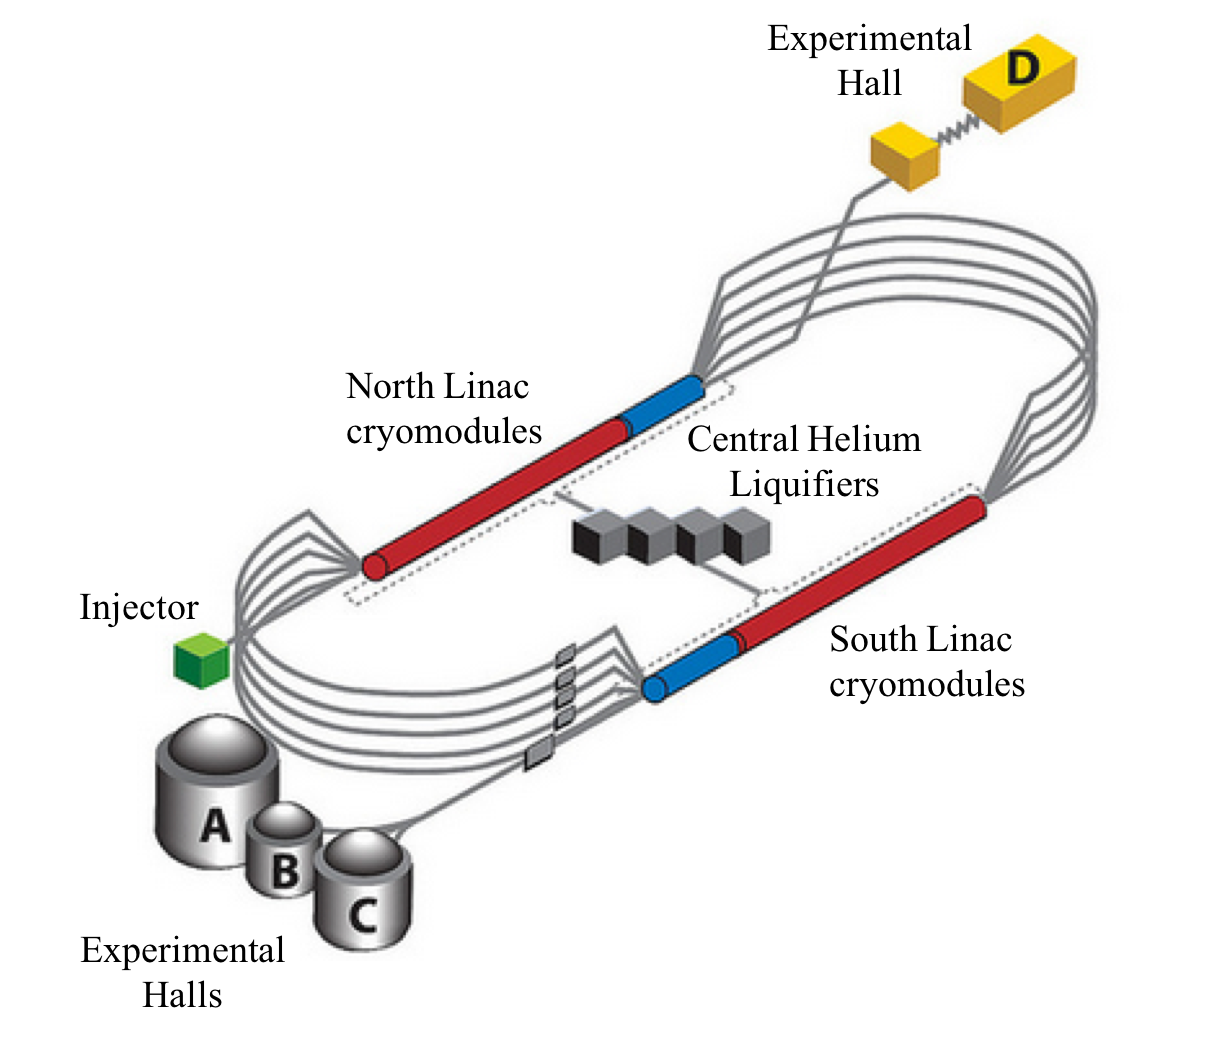
\includegraphics[width=0.75\textwidth]{pics/experiment/cebafLabel.png}
  \caption[CEBAF accelerator]{The CEBAF accelerator was upgraded prior to the HPS experiment to include additional cryomodules and central helium liquifier (CHL) for higher energy, a fifth pass, and a fourth experimental hall.}
  \label{Figure:cebaf}
\end{figure}

The injector energy is 100~MeV, designed for a maximum of five passes (upgraded from four passes) with an energy per pass of 2.2~GeV (upgraded from 1.1~GeV). These upgrades double the maximum energy output of the accelerator. While the accelerator frequency operates at 1500~MHz, a new 750~MHz RF separator was installed in order to provide beam to all four halls simultaneously. With these upgrades, the halls can receive the beam at 250 or 500~MHz and operate at different energies \cite{kazimi}. 

HPS is the first experiment to run in Hall B after the accelerator was upgraded. After a problem occurred in one CHL during the Engineering Run in the spring of 2015, HPS obtained dedicated beam time as one of the few experiments that could continue to take physics data with the accelerator operating at a single pass using the remaining CHL. The resulting energy for the Engineering Run, 1.05~GeV, would have been impossible to obtain with the simultaneous running of other experiments requiring 2.2~GeV per pass.  


\section{Beamline}
The HPS experiment is installed in the downstream alcove of experimental Hall B at Jefferson Lab as shown in Fig.~\ref{Figure:hallB}~\cite{Takashi}. Due to the planned construction of the CLAS12 detector in Hall B as part of the 12~GeV upgrade, HPS running was planned for nights and weekends when running beam through the hall would not interfere with CLAS12 construction. After the failure of the second CHL, HPS received dedicated, continuous running during May of 2015 in support of the Engineering Run. 

\begin{figure}[H]
  \centering
      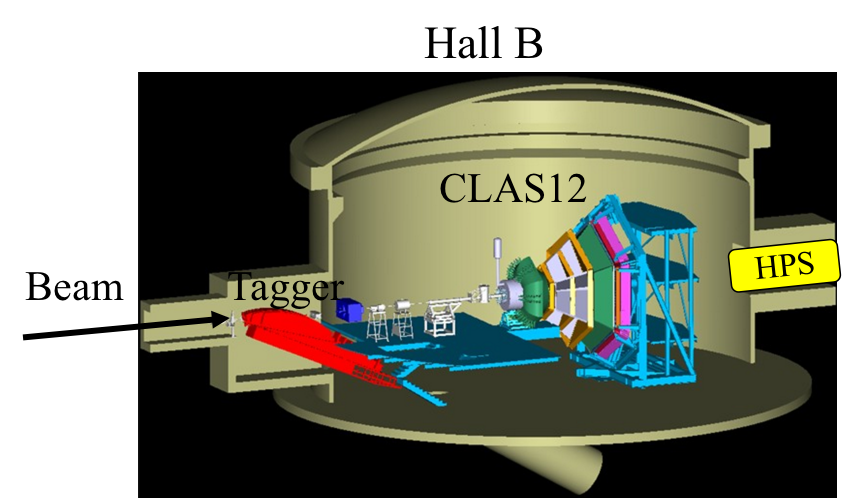
\includegraphics[width=0.6\textwidth]{pics/experiment/hallB.png}
  \caption[HPS location in Hall B]{The HPS experiment is in the downstream alcove of Hall B and ran while not interfering with CLAS12 construction.}
  \label{Figure:hallB}
\end{figure}

The tagger magnet as depicted in Fig.~\ref{Figure:hallB} was used for initial beam tuning from the accelerator before sending the beam through to the HPS detectors. By energizing the tagger magnet, the electron beam was visible at the tagger dump viewer and could be aligned at the center of the viewer. Harp scans were performed to measure the position and width of the beam spot after the beam appeared to be in reasonable alignment~\cite{Takashi}. Once the harp scans showed the beam to be of an acceptable size and position upstream of HPS, the tagger magnet was de-gaussed for HPS running. Without the tagger magnet on, the electron beam enters the hall in vacuum and passes through the hall to the HPS setup as shown in Fig.~\ref{Figure:hpsBeamline}. 

\begin{figure}[H]
  \centering
      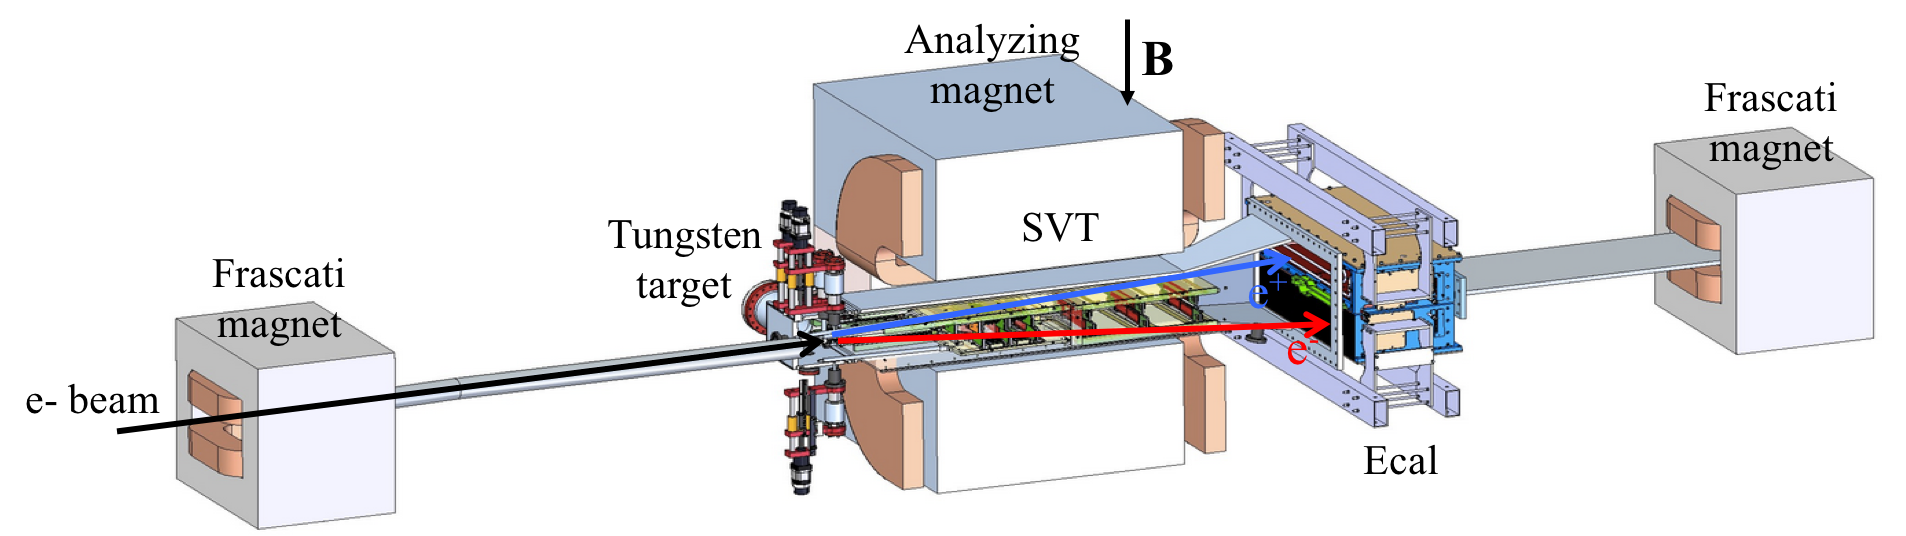
\includegraphics[width=1.0\textwidth]{pics/experiment/hpsBeamline.png}
  \caption[HPS beamline]{The SVT and target are contained within the analyzing magnet. Particles created from the interaction of the beam at the target pass through the SVT before depositing their energy into the ECal.}
  \label{Figure:hpsBeamline}
\end{figure}

The HPS setup consists of a three-dipole chicane with fields in the vertical direction, perpendicular to the Hall B floor. The target and the SVT are housed in the central magnet known as the pair spectrometer, or analyzing magnet. The pair spectrometer has a pole length of 91.44~cm and width of 45.72~cm. For 2.2~GeV electrons, the central magnetic field of the pair spectrometer magnet is 0.5~T~\cite{Takashi}. For other beam energies, the analyzing magnet magnetic field is scaled accordingly. In the Engineering Run in May 2015, with a beam energy of 1.056~GeV, the pair spectrometer had a central field value of 0.24~T. The Frascati magnets, one on each side of the analyzing magnet, have magnetic fields opposite to that of the analyzing magnet such that the integrated field value over the length of the pole value of each Frascati is half of the integrated field value of the analyzing magnet. This ensures that the beam will end at the same location whether the chicane is energized or not and that the trajectory of beam energy electrons in the magnetic field is consistent across different beam energies. The magnetic field of the HPS beam line in the chicane is shown in Fig.~\ref{Figure:bField}.

\begin{figure}[H]
  \centering
      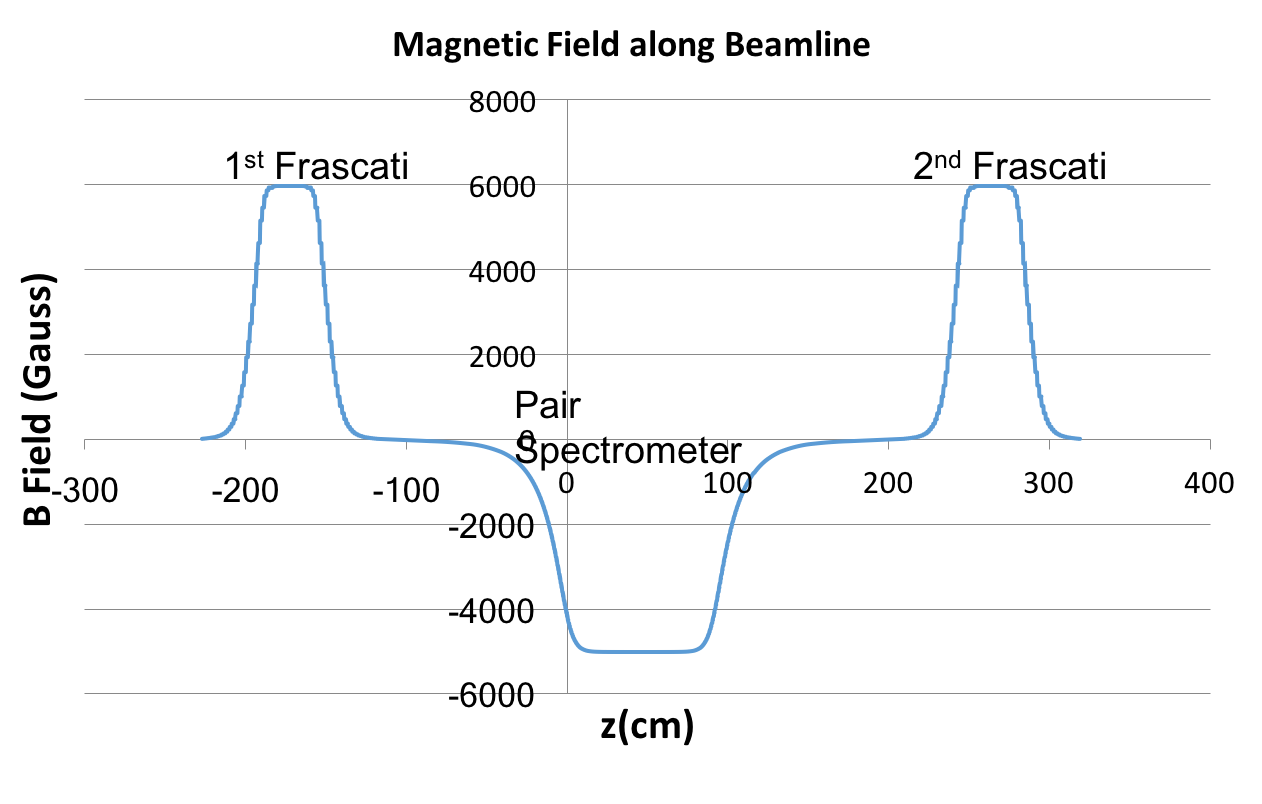
\includegraphics[width=1.0\textwidth]{pics/experiment/bfield.png}
  \caption[HPS magnetic fields]{The dipole field values for 2.2~GeV running.}
  \label{Figure:bField}
\end{figure}

The trajectory and position of particles inside the magnetic field was studied using magetic field mappings from experimentally obtained measurements that included fringe field effects. The positions of the pair spectrometer magnet with respect to the Frascati magnets was determined from these field mappings. The horizontal trajectory of a beam energy electron as affected by the magnetic field is shown in Fig.~\ref{Figure:trajectory}.

\begin{figure}[H]
  \centering
      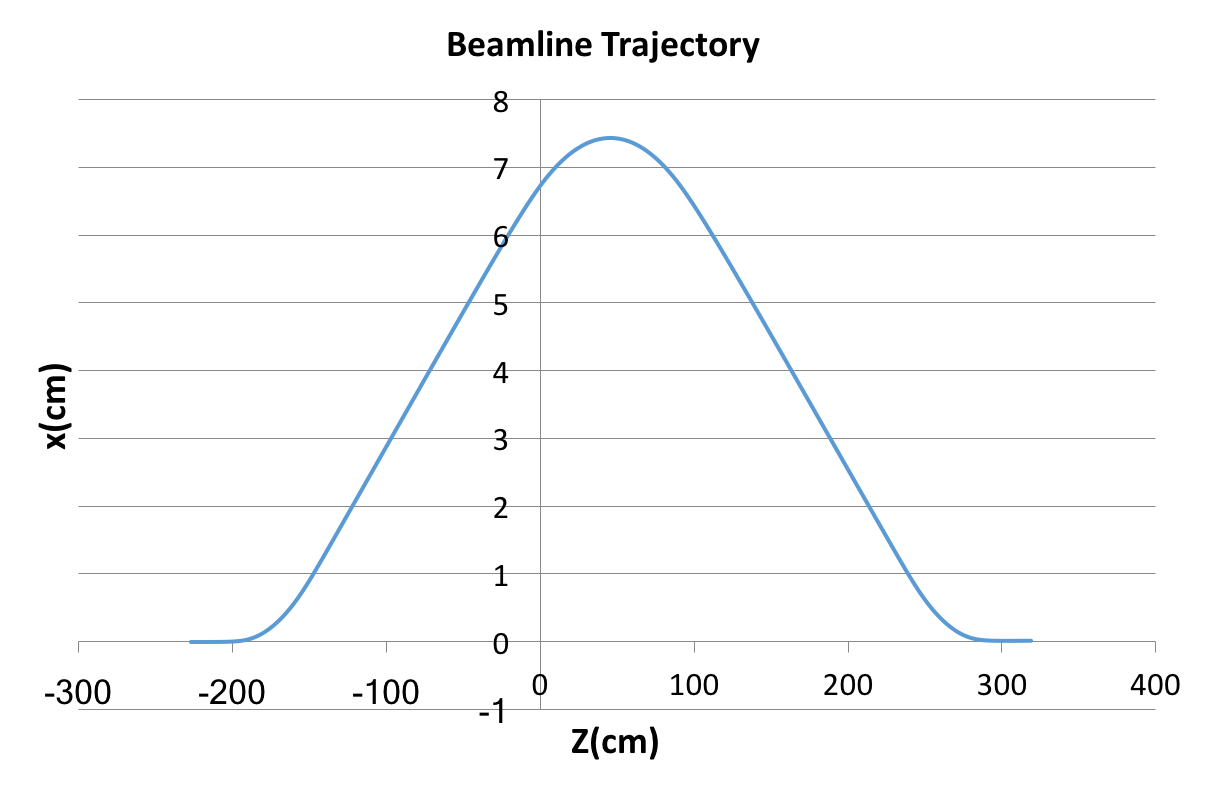
\includegraphics[width=1.0\textwidth]{pics/experiment/feetrajectory.png}
  \caption[Charged particle trajectory in HPS beamline]{The horizontal trajectory of a 2.2~GeV electron through the three dipole chicane where the target position is at Z=0.}
  \label{Figure:trajectory}
\end{figure}

In Fig.~\ref{Figure:trajectory}, the target position is where the $z$ position is zero. The entry angle at the target was also studied and determined to be approximately 30.5~mrad. At 70~cm from the target, the pair spectrometer magnet and vacuum chamber are centered on the position of the photon trajectory from the target such that the photons pass unobstructed through all subsequent vacuum chambers. The pair spectrometer magnet was placed 8.87~cm beam left, thus placing the HPS target position 2.14~cm to the right of the magnet center line. By modeling the vacuum chambers and magnetic fields in the GEant4 Monte Carlo (GEMC) framework, the particle trajectories through the HPS beam line can be observed as in Fig.~\ref{Figure:gemc}.

\begin{figure}[H]
  \centering
      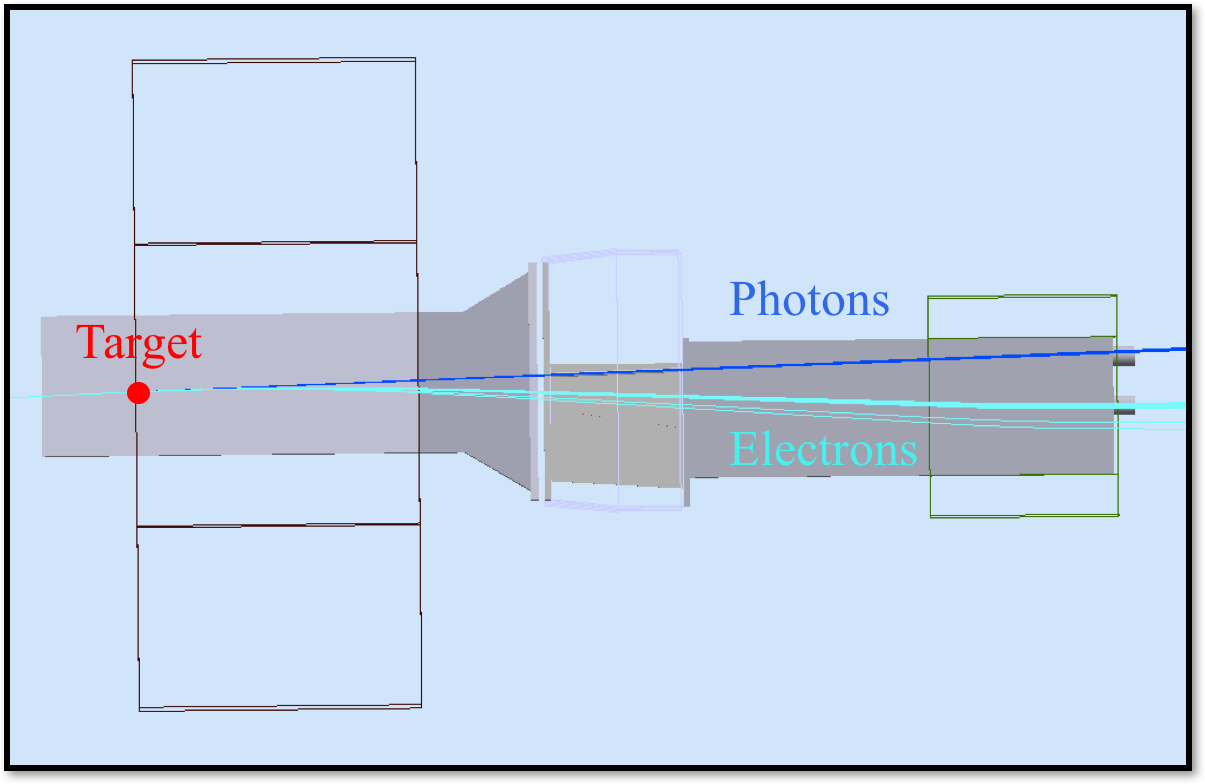
\includegraphics[width=0.8\textwidth]{pics/experiment/beamlineGemc.png}
  \caption[HPS beamline simulation in GEMC]{A bird's eye view of the HPS beam line shows the straight line trajectory of the photons from the HPS target through the SVT, ECal, and last vacuum chamber. The trajectory of the electrons in the magnetic field can be seen as clearly passing through the relevant cut outs in the vacuum chambers.}
  \label{Figure:gemc}
\end{figure}
 
As shown in ~\ref{Figure:gemc}, the beam energy electrons clearly pass through the exit hole of the last vacuum chamber (contained in the second Frascati dipole) and continue traveling to the Faraday cup where the beam charge can be measured. The beam line was modeled in GEMC and, in real running, utilized a multitude of monitors to ensure clear passage of the beam.

The passage of the beam through the HPS beam line was monitored using beam position monitors (BPMs), wire scans with halo counters, beam viewers, and a Faraday cup. The three upstream nA BPMs give continuous beam current and position readings. These BPMs can indicate that the beam is scraping the beam pipe when the current readings are fluctuate and differ with respect to each other. The current readings from the BPMs were compared to the current reading at the Faraday Cup (located downstream of the HPS beam line at the dump). When the beam current is at 50~nA or below, the reading at the Faraday Cup current is roughly the same as the current read out by the upstream BPMs and indicates no beam scraping in the beam pipe. When operating at currents above 50~nA, it was standard to insert a beam blocker in front of the Faraday Cup in order to protect it. The beam stopper would then create an offset in the Faraday Cup current readout and the actual beam current. Additionally, a viewer screen at the Faraday Cup was used to show the beam position. HPS used a florescent screen that showed the position of the beam by emitting light at the particular point where the beam passed on the screen. A video camera streaming a view of the screen was used for remotely observing the relative beam position on the screen.  

Harp scans measure the current and position of the beam through interaction with the beam (as compared to the passive, continuous readout employed through the BPMs). A harp scan moves wires through the beam vertically, horizontally, and diagonally while  downstream halo counters measure the scattered beam electron spray. The halo counters are photomultiplier tubes (PMT) strapped around the beam pipe line. The intensity of the electron spray detected by the PMTs is proportional to the beam charge that the wire interacts with. A typical harp scan from the Engineering Run is shown in Fig.~\ref{Figure:harpScan}.

\begin{figure}[H]
  \centering
      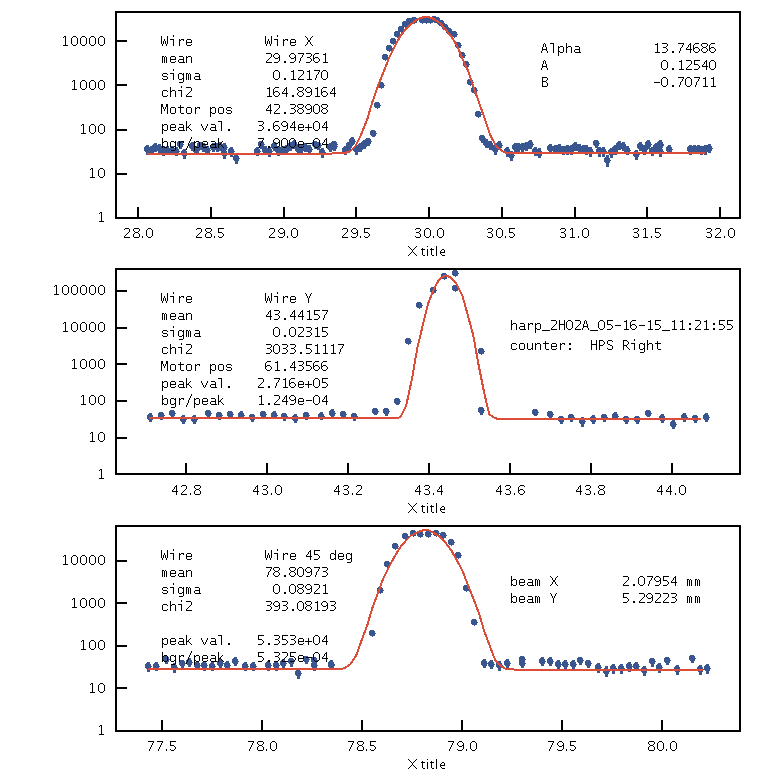
\includegraphics[width=1.0\textwidth]{pics/experiment/harpScan.png}
  \caption[Beam profile from harp scan during 2015 run]{Harp scan showing the beam profile during May 2015 running. This particular harp scan is in the Hall B logbook, entry 3341231. The beamline profile in this scan is 122$\mu$m wide in $x$ by 23$\mu$m in $y$.}
  \label{Figure:harpScan}
\end{figure}

In Fig.~\ref{Figure:harpScan}, the beam profile is characteristically narrower in $y$ (vertically) than in $x$ (horizontally). The proposed beam profile for the HPS experiment was 50~$\mu$m in $y$ and 300~$\mu$m in $x$ in order to prevent overheating at the target and allow for precise vertex reconstruction. While overheating was not a limiting factor in the experiment, most of the 2015 running had a beam profile of no larger than 50~$\mu$m in $y$ and 150~$\mu$m in $x$. 

\subsection{Target}

The primary HPS target is a thin tungsten foil that is mounted on a support frame having the capability to be fully retracted from the beam when not in use. For proposed 1.1~GeV and 2.2~GeV running, the design thickness of the target tungsten foil is 0.125$\%$ radiation lengths (approximately 4~$\mu$m of tungsten). The measured thickness of the actual target was 0.116$\%$. Mounted on the same frame is a tungsten target of 0.25$\%$ radiation lengths for future running at 4.4~GeV and 6.6~GeV. The target support frame inserts the foil target from above the beam using a stepping motor linear actuator. By necessity, the bottom of the target foil is free-standing so that the target can be inserted into the active beam without interruption.  

\subsection{Collimator}

A collimator is used in the HPS beamline in order to protect the silicon strips of the SVT detector in the event of the beam moving vertically from its nominal position. The collimator is a 1~cm thick tungsten plate with different sized holes through which the beam can pass. Should the beam drift vertically from its nominal position, the collimator would be able to absorb the beam and protect the silicon before the machine fast shutdown (FSD) would be triggered by excess counts in the beam halo counters. For the 2015 run, the 4~mm collimator hole was used. 


\section{Silicon Vertex Tracker}
The Silicon Vertex Tracker (SVT) is the key detector of the HPS experiment for measuring particle momentum and trajectories through a magnetic field in order to reconstruct the invariant mass and the vertex position of the $e+e-$ pair. The SVT is composed of six layers of 0.7$\%$ radiation length-thick silicon placed downstream of the target and housed in a vacuum chamber within the analyzing magnet. The SVT is separated into top and bottom halves with a 15~mrad opening angle and the first layer of the SVT at $\pm$0.5~mm from the active beam. A drawing of the SVT is shown in Figure~\ref{Figure:svt}.

\begin{figure}[H]
  \centering
      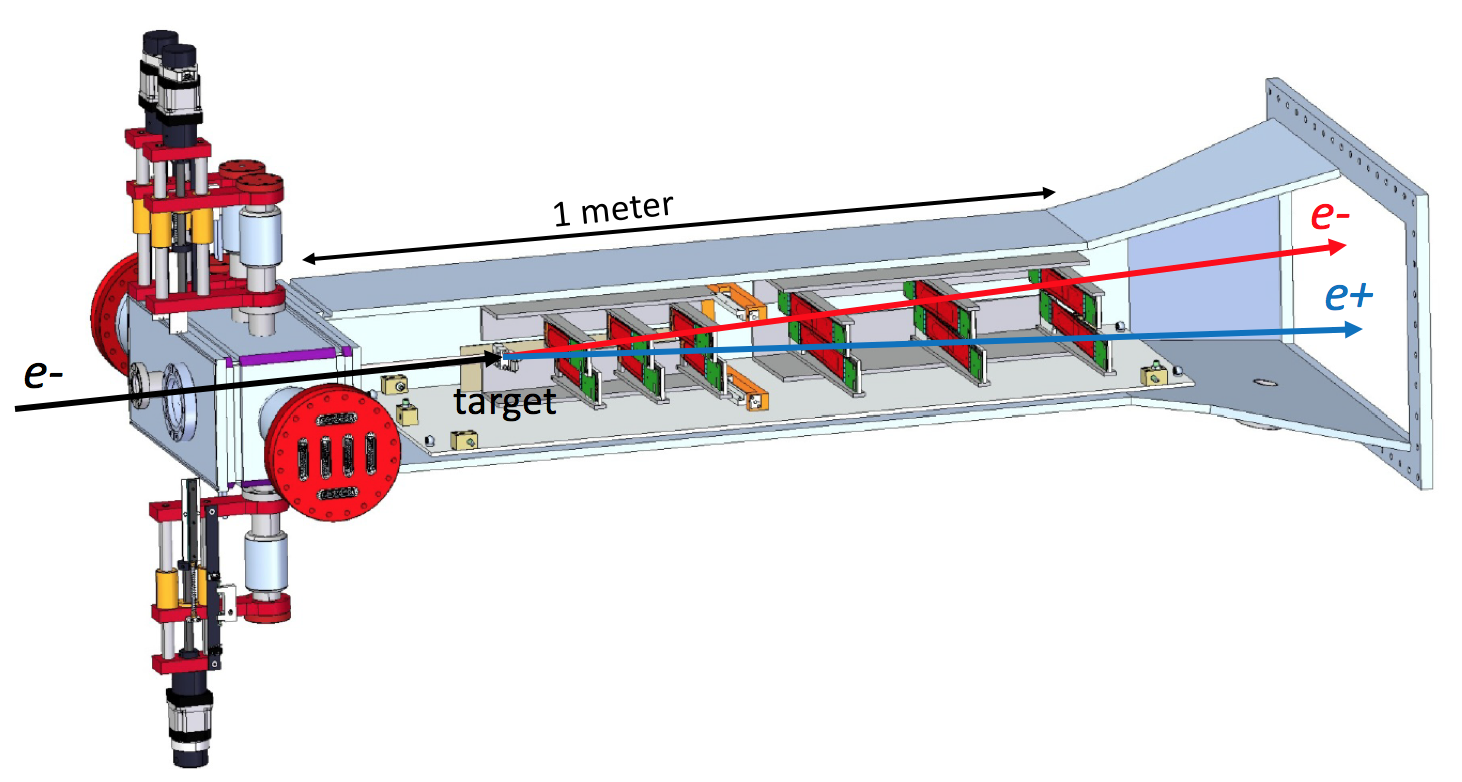
\includegraphics[width=1.0\textwidth]{pics/experiment/svt.png}
  \caption[Rendering of the HPS SVT]{A rendering of the HPS SVT. The beam enters from the left through the vacuum box. The silicon sensors are shown in red, and the hybrid readout boards are shown in green.}
  \label{Figure:svt}
\end{figure}


The SVT, as shown in Figure~\ref{Figure:svt}, is housed in a magnetic field such that particles are bent horizontally (field acts downward). Each of the six layers is composed of two strips capable of measuring a hit position in one dimension. By setting the strips at a stereo angle with respect to one another, each layer of the SVT is capable of three-dimensional hit reconstruction. The first three layers of the SVT are one silicon strip sensor-wide and have a stereo angle of 100~mrad between the strips. The last three layers of the SVT are two strip sensors-wide in order to better match the Ecal acceptance. The stereo angle between the sensors in layers four through six is 50~mrad. The axial sensors are oriented along the bend plane direction whereas the stereo sensors are angled with the lower end closer to the beam plane on the positron side where the background are less intense. The different stereo angles are used to eliminate ghost hits that can generate ghost tracks. The first five layers of the SVT cover the Ecal acceptance while the sixth layer has a slightly reduced acceptance but can be used to improve track reconstruction. The full track reconstruction only requires five hits per track in order to pick up tracks that may be missing hits due to an inefficiency. \\
\indent The hybrid readout boards on each sensor house the APV25 readout chips that connect the sensor to the data acquisition (DAQ) system. The power to the APV25 chips is supplied through the hybrid, and the temperature of the strip is also actively monitored at the hybrid. The heat generated by the operating hybrid is pulled out through the aluminum support structure. As the sensors are cooled for operation, the support structure and sensor contract at slightly different rates. In order to adjust and maintain the sensor at a constant tension, one end of the sensor is attached to a spring pivot in order to maintain rigidity. The assembly of a silicon sensor is shown in Figure~\ref{Figure:svtAssembly}.
\begin{figure}[H]
  \centering
      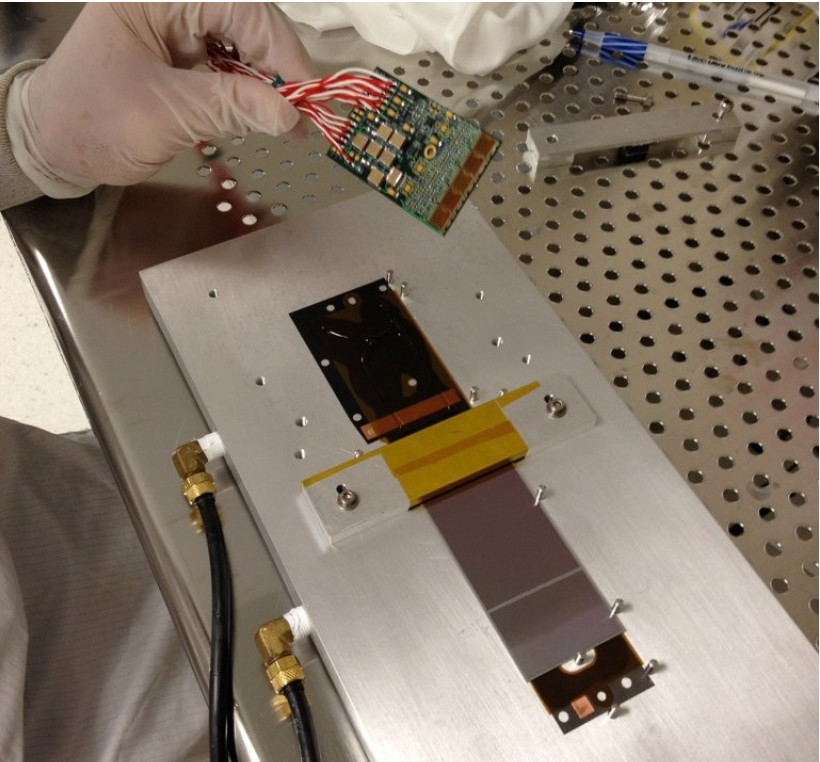
\includegraphics[width=0.5\textwidth]{pics/experiment/svtSensorAssembly.png}
  \caption[Assembly of a half module of the SVT ]{A half module is being assembled for Layers 1-3 of the SVT. A readout hybrid with the APV25 chips is being attached to the frame along the silicon sensor.~\cite{collaboration_heavy_2013}}
  \label{Figure:svtAssembly}
\end{figure}
The APV25 samples the strips every 24~ns and stores the results in a pipeline. Once a trigger is received, the corresponding channel pipeline is readout. The readout yields six samples at 24~ns intervals that can be fit to reconstruct the waveform. A 4-pole functional fit was used to extract the time and amplitude of the corresponding hit. A latency time that is configured in the SVT DAQ is used to correctly determine which channel pipelines are readout that correspond to the trigger. The latency time is approximately equal to the time delay of the trigger. Some early data in the Engineering Run was lost due to incorrectly timing in the SVT latency. 


\section{Electromagnetic Calorimeter}
The HPS Ecal is a homogeneous calorimeter composed for 442 trapezoidal PbWO$_4$ scintillating crystals each readout by a large area avalanche photodiode (APD) attached to the back of each crystal. The Ecal triggers events and provides particle energy and timing information. 

The crystals are re-purposed from the former CLAS Inner Calorimeter detector and have been upgraded with larger avalanche photodiodes. Each crystal is trapezoidal in shape and 16~cm long with the front (back) face 1.3$\times$1.3~mm$^2$ (1.6$\times$1.6~mm$^2$). The calorimeter layout is shown in Fig.~\ref{Figure:ecalface}. 

\begin{figure}[thb]
  \centering
      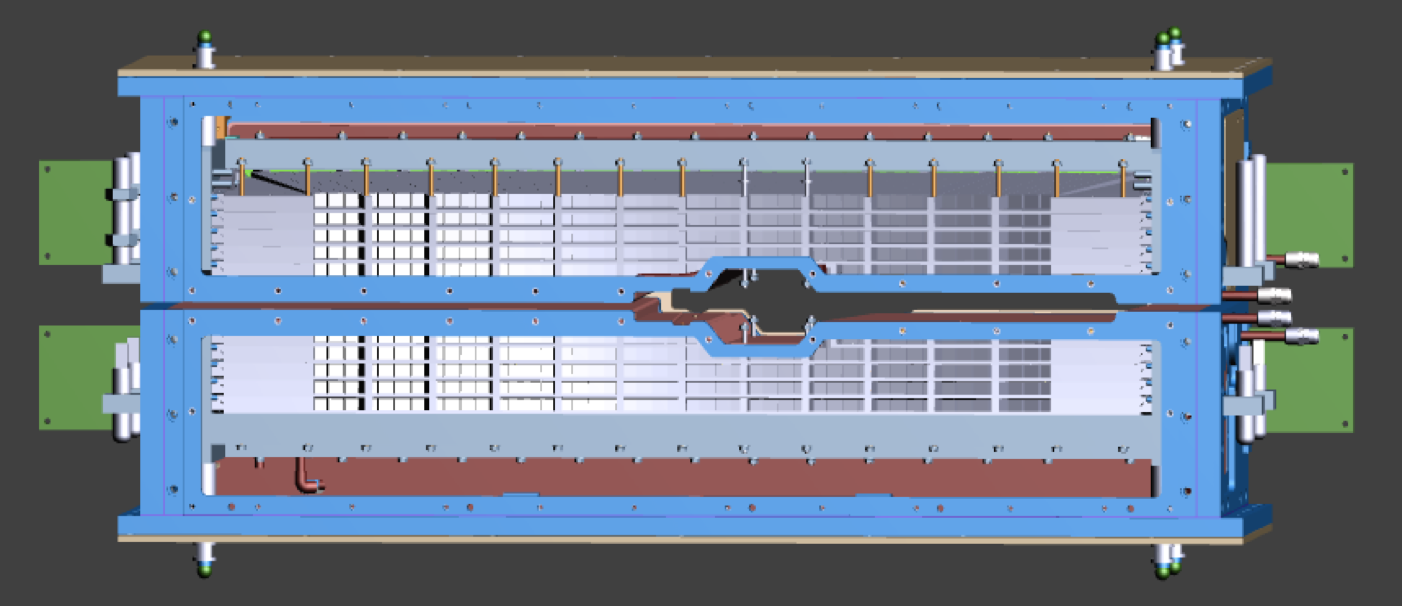
\includegraphics[width=0.85\textwidth]{pics/experiment/ecalface.png}
  \caption[Drawing of the Ecal assembly face]{Drawing of the Ecal assembly face, looking downstream with the beam direction. The Ecal is assembled in two vertical halves and has a gap in between allowing for the electron and photon beams as well as the sheet of flame.}
  \label{Figure:ecalface}
\end{figure}

The Ecal in constructed as two separate vertical halves in order to avoid the 15~mrad vertical zone of excessive electromagnetic background along the beam line. The crystals in each half are arranged in five layers of 46 crystals. The layer of crystals closest to the beam in each half has nine crystals removed to allow for the passing of the electron beam. The two halves of the Ecal rest at 2~cm vertical distance from the  horizontal electron beam plane.

\begin{figure}[thb]
  \centering
      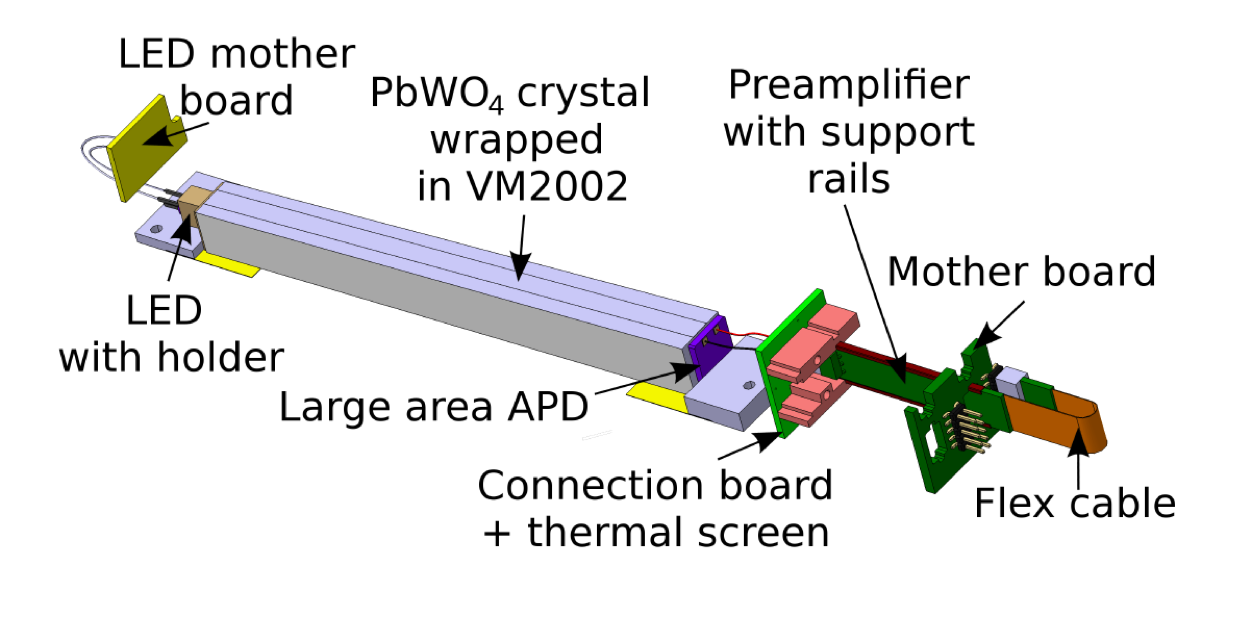
\includegraphics[width=0.85\textwidth]{pics/experiment/crystal.png}
  \caption[Single Ecal module]{Drawing of an Ecal crystal in readout configuration.}
  \label{Figure:crystal}
\end{figure}

Each crystal is wrapped in a VM2002 reflecting foil in order to increase light collection. The original APDs used by the the Inner Calorimeter had a surface area of 5$\times$5~mm$^2$, but these were upgraded for HPS running by replacing each original APD with a large area APD (model S8664-1010) of surface area 10$\times$10~mm$^2$. The upgraded large area APDs are capable of collecting four times the light as compared to the same energy deposited into the old APDs. The larger signals require less electronic amplification of the signal and improve the signal-to noise-ratio. Ultimately, the upgrade in electronics requires a lower energy threshold for module readout and improves energy resolution. 

As a particle deposits its energy into the scintillating crystal, the photons are collected at the back of the crystal by the APD and converted into an electronic signal via the photoelectric effect. Each APD is attached by a twisted pair connector to a preamplifier which converts the signal current to voltage and has low input impedence and noise.  

\begin{figure}[H]
  \centering
      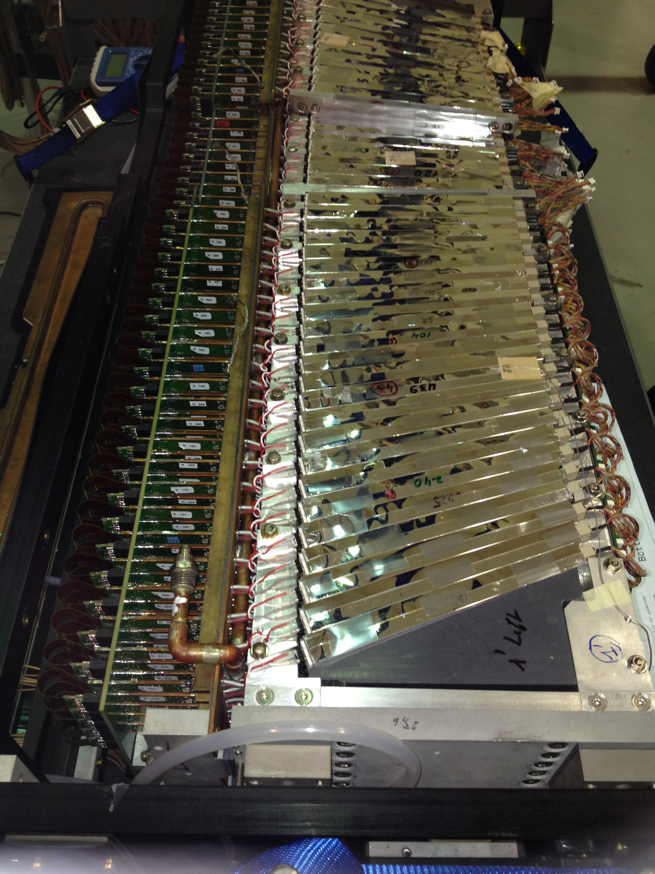
\includegraphics[width=0.5\textwidth]{pics/experiment/ecalAssembly1.png}
  \caption[Photograph of Ecal crystals during assembly]{Photograph taken during assembly of the Ecal from above. The preamplifiers attached to each crystal are shown on the left. As single layer of wrapped crystals are shown in their tray and the LEDs attached to each crystal are shown on the right.}
  \label{Figure:ecalAssembly1}
\end{figure}

The gain of the APDs and the scintillation of the crystals in the Ecal are temperature-dependent effects. An Anova A-40 external chiller operating at 17$\degree$C pumps cool water through copper cooling pipes that run along the inside of the Ecal at the top, bottom, front and back face of the crystal structure. The internal temperature of the Ecal was monitored using sixteen thermocouples located at various locations within the Ecal structure. The thermocouples are readout using an Omega D5000 series transmitters. Both devices are connected through RS-232 serial communications for external monitoring and alarms should the temperature change significantly.

Low voltage is supplied to the preamplifiers via an Agilent 6221 operating at 5~V and approximately 4.1~A when all preamplifiers are connected. The high voltage to each of the 52 APD groups is supplied by the CAEN A1520P modules in the SY4527 mainframe. Both voltage suppliers are monitored and accessible for remote operations.  


\subsection{Light Monitoring System}
The Light Monitoring System (LMS) is a design upgrade addition to the Ecal consisting of a bi-color LED attached to the front of each Ecal module and capable of being controlled remotely. PbWO$_4$ scintillating crystals are relatively radiation tolerant but have a known decrease in light yield after exposure to radiation \cite{Batarin}. This effect is non-uniform in the Ecal as a module's geometrical position relative to the beam will result in different levels of radiation. The LMS has the ability to turn individual modules on and off independently which proved useful in checking each channel's functionality and correct cabling. The use of LEDs in a monitoring system for the PbWO$_4$ modules is particularly advantageous because the LEDs can be selected such that the shape and duration of the emitted flash can generate a pulse shape similar to the scintillation effect in the crystal \cite{Battaglieri}.

Each crystal has a plastic LED holder glued to the front that contains a bi-color LED, model RAPID 56-0352, capable of emitting red and blue light. The use of two different colors allows for the study of different effects in the Ecal modules. The blue LED has a wavelength close to the 430~nm emission peak of PbWO$_4$  \cite{Battaglieri} and is used to check for radiation damage in the crystal as this spectrum would be most affected. The red light is not susceptible to the radiation effects in the crystals, but is useful for checking the stability of the  APD gains. 

The LMS consists of four driver boards on each half of the Ecal. The four driver boards on each half are connected to one of two main controllers, and each driver can turn on a single LED at a time. The controllers provide communication with the LMS through ethernet and USB interfaces. The controller board for the top half of the Ecal also contains the master clock signal that sets the rate at which the LEDs flash. This clock signal is sent to the bottom controller so that the driver boards on the bottom half of the Ecal can flash at the same rate, and the clock signal is used to trigger LED events when the DAQ is used. 


During the initial assembly of the Ecal, the LEDs were used to study the cross talk between Ecal modules. The cross talk between channels was found to be at the level of 2$\pm$1$\%$ and generally occurred in modules of the same row to the immediate left and right of the triggered module. The effect most likely appears due to light leakage out the back face of the crystal where the APD does not cover the entire surface.

The raw waveform response from a red LED signal in a single Ecal module is shown in Fig.~\ref{Figure:redSignal}. The raw units are given in mV which are a factor of four times less than the units of FADC.

\begin{figure}[H]
  \centering
      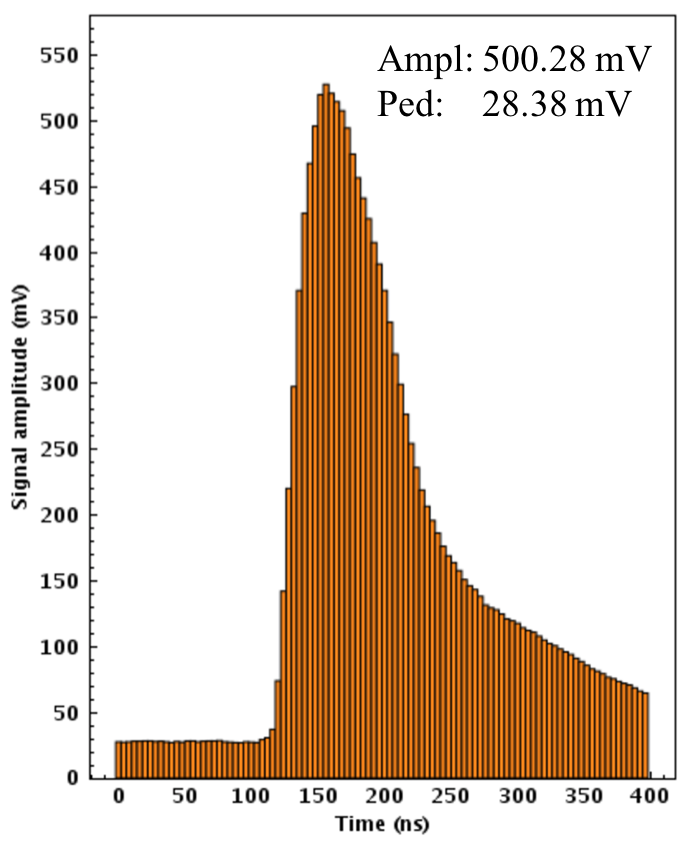
\includegraphics[width=0.5\textwidth]{pics/experiment/ledSignal.png}
  \caption[LED signal in Ecal FADC]{A red LED in a single Ecal module as readout through the FADC.}
  \label{Figure:redSignal}
\end{figure}

Before and after periods of long beam running, an LED test was run so that the general gains of the Ecal could be checked. The LED test ran a sequence of red and blue LEDs so that the characteristic response of each module was measured. The typical results from an LED test are shown in Fig.~\ref{Figure:redCompare}.

\begin{figure}[H]
  \centering
      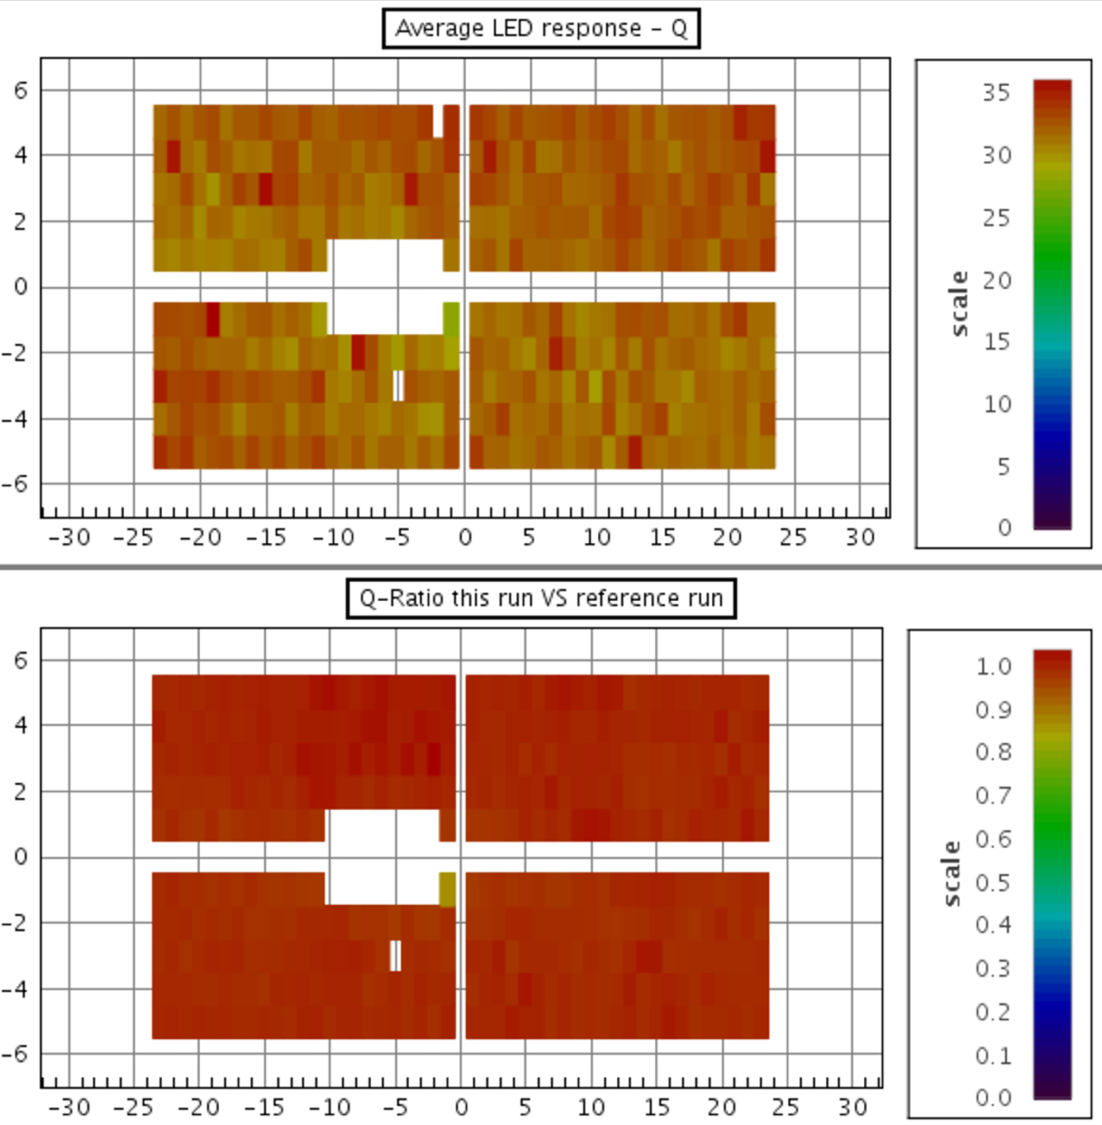
\includegraphics[width=0.5\textwidth]{pics/experiment/ledCompare.png}
  \caption[Results of a single LED run]{The top shows the LED response in each crystal for a specific LED run. The bottom compares each crystal with a its database value as stored from a previous LED run.}
  \label{Figure:redCompare}
\end{figure}

As shown in Fig.~\ref{Figure:redCompare}, the individual Ecal module response is given as the pulse-integral in units of GeV. The response values for individual crystals have large units of energy because the LED pulse is so much longer than an actual scintillation pulse in the crystal. A LED test can show differences in the gains of individual crystals on the order of $1\%$ when compared to previous LED test results. During the spring 2015 running, a 5$\%$ change in gains occurred over the course of establishing production beam between February and April. This change was seen in LED response studies in addition to the gains obtained with cosmic energy calibration.


\subsection{Avalanche Photodiodes}
The ECal upgraded by installing large area Hamamatsu S8664-3189 APDs for readout. APDs were used for reading out the ECal modules due to their ability to operate in the fringe magnetic field of the HPS beam line. Both the Institut de Physique Nucleaire d'Orsay (IPN) and Instituto Nazionale di Fisica Nucleare (INFN) groups in the HPS collaboration purchased the large area APDs for upgrade. As the IPN group re-designed the motherboards for the upgrade, INFN developed the testing apparatus so that the gain of each APD could be characterized and sorted into one of 52 high voltage groups to minimize response variations. The large area APDs are shown in Fig.~\ref{Figure:apd}.

\begin{figure}[H]
  \centering
      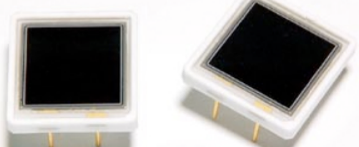
\includegraphics[width=0.4\textwidth]{pics/experiment/apd.png}
  \caption[Hamamatsu S8664-3189 large area APDs]{The Hamamatsu S8664-3189 large area APDs.}
  \label{Figure:apd}
\end{figure}

APDs are reverse-biased diodes with an internal high electric field that multiplies the electrons through an avalanche mechanism.  The characteristic gain of an APD depends on the temperature of the environment due to the interaction of the electrons with the phonons. The gain is inversely correlated with temperature.  The APD gains have a linear dependence on both voltage and temperature. Prior to grouping the APDs for installation in the ECal, each APD was tested and bench marked to check for quality and optimal operating voltage in order to achieve a pre-selected gain of 150. The testing apparatus was designed and installed by the group from INFN as the same procedure was used in the construction of the Forward Tagger \cite{celentano_2014}. The bench marking apparatus is shown in Fig.~\ref{Figure:apdtest}.

\begin{figure}[H]
  \centering
      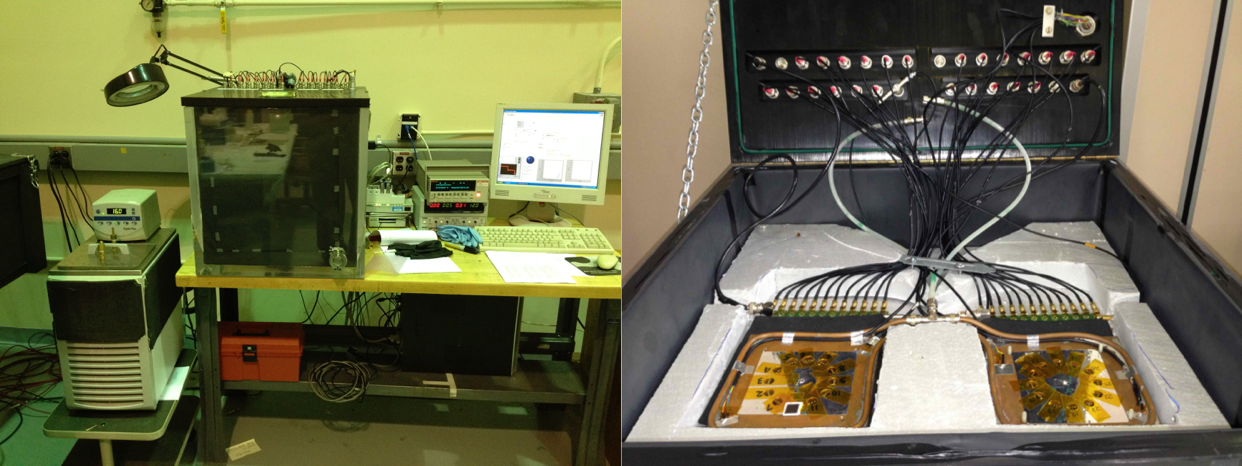
\includegraphics[width=0.7\textwidth]{pics/experiment/apdtests.png}
  \caption[Testing assembly for large area APDs]{On the left, the testing setup is shown and includes a chiller, the light-tight plastic box that contains the LEDs and APDs, an electrometer, and the data acquisition. On the right, the setup inside of the light-tight plastic box is shown that contains a copper cooling plate to maintain the chiller temperature, 10 slots on each side to hold APDs, and the LED in the center of each half.}
  \label{Figure:apdtest}
\end{figure}

In order to avoid condensation on the cooling lines, the temperature range for conducting the tests was limited to 16$\degree$C,18$\degree$C, and 20$\degree$C. During the testing, the current in each APD is measured by the electrometer with the LED on and off while stepping through a range of voltages. The measured dark and light currents for an individual APD during testing are shown in Fig.~\ref{Figure:apdcurrent}.

\begin{figure}[H]
  \centering
      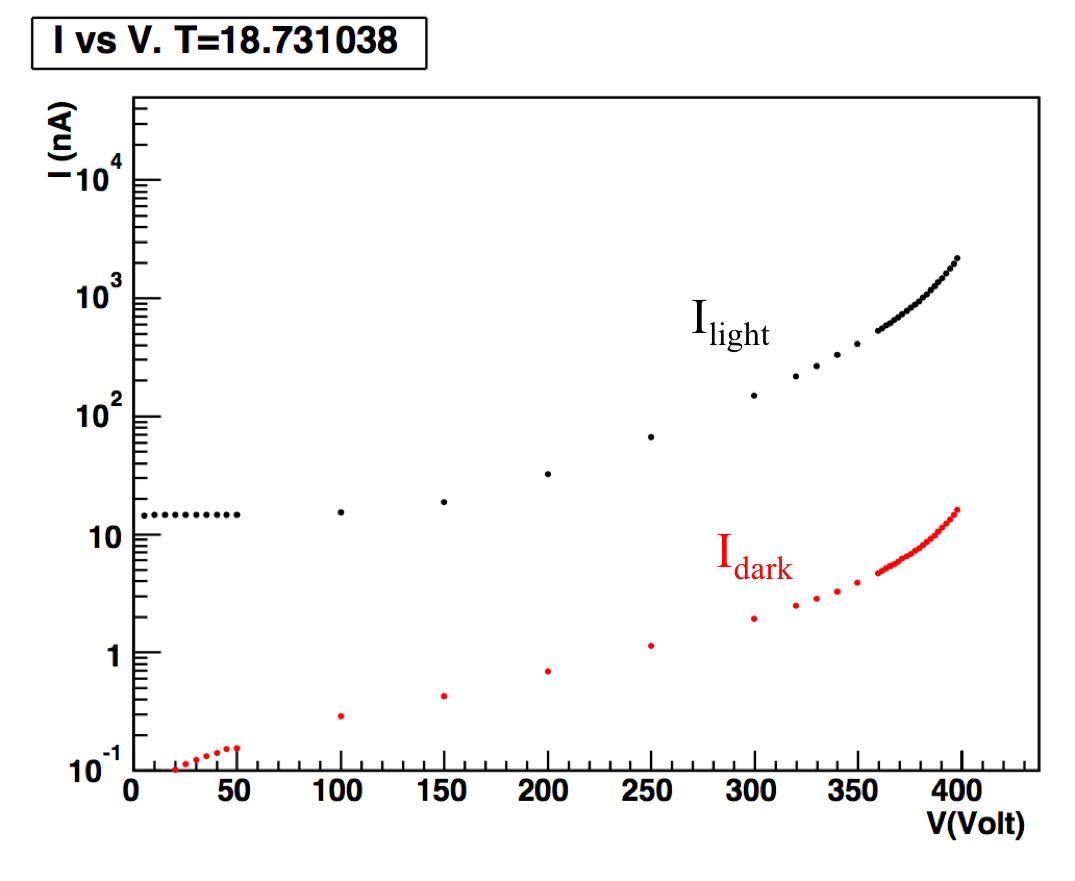
\includegraphics[width=0.5\textwidth]{pics/experiment/apdcurrent.png}
  \caption[APD current draw versus voltage with LED on and off]{The current measured from an individual APD as tested over a range of voltages with both the LED on and off. The measured temperature at the APD for this particular measurement was 18.7~$\degree$C.}
  \label{Figure:apdcurrent}
\end{figure}

The full characterization of the APD gain is calculated by the following relation:

\begin{equation}
	\label{eq:apdgain}
	Gain = \dfrac{I_{light}(V)-I_{dark}(V)}{I_{light}(G=1)-I_{dark}(G=1)} 
\end{equation}

The gain is determined to be 1 when the avalanche mechanism is not present. The $I_{light}(G=1)$ in Eq.~\eqref{eq:gain} the corresponding light current and $I_{dark}(G=1)$ is the measured dark current when the gain is 1. Using this relation, the gain can be characterized for all measured dark currents and should have a linear relation. This relationship is shown in Fig.~\ref{Figure:apdIvG}.

\begin{figure}[H]
  \centering
      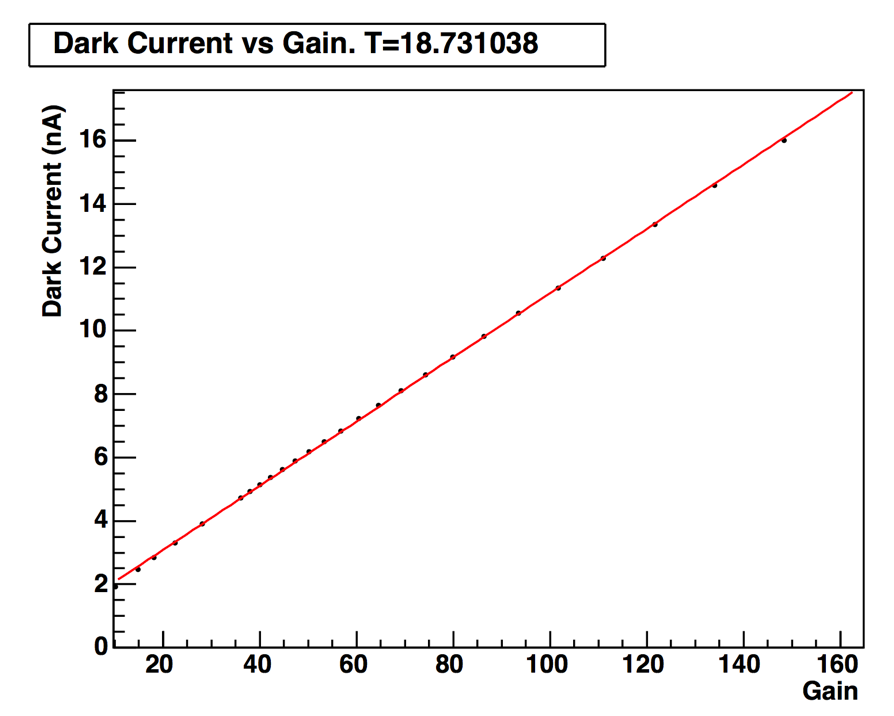
\includegraphics[width=0.5\textwidth]{pics/experiment/apdIvG.png}
  \caption[APD measured dark current as a function of gain]{The current measured from an individual APD as tested over a range of voltages with both the LED on and off. The measured temperature at the APD for this particular measurement was 18.7~$\degree$C.}
  \label{Figure:apdIvG}
\end{figure}

If the relationship between the dark current and the gain is not linear, as shown in Fig.~\ref{Figure:apdIvG}, then the APD was re-tested to ensure quality. APDs were placed into 52 common voltage groups ranging from as little as two to a maximum of ten APDs in each group in order to minimize gain variations across the ECal. The grouping temperature was chosen to be 18~$\degree$C in order to avoid condensation in the cooling lines of the ECal. The optimal voltage for each APD at 18~$\degree$C and a pre-selected gain of 150 can be extrapolated as shown in Fig.~\ref{Figure:apdTV}.

\begin{figure}[H]
  \centering
      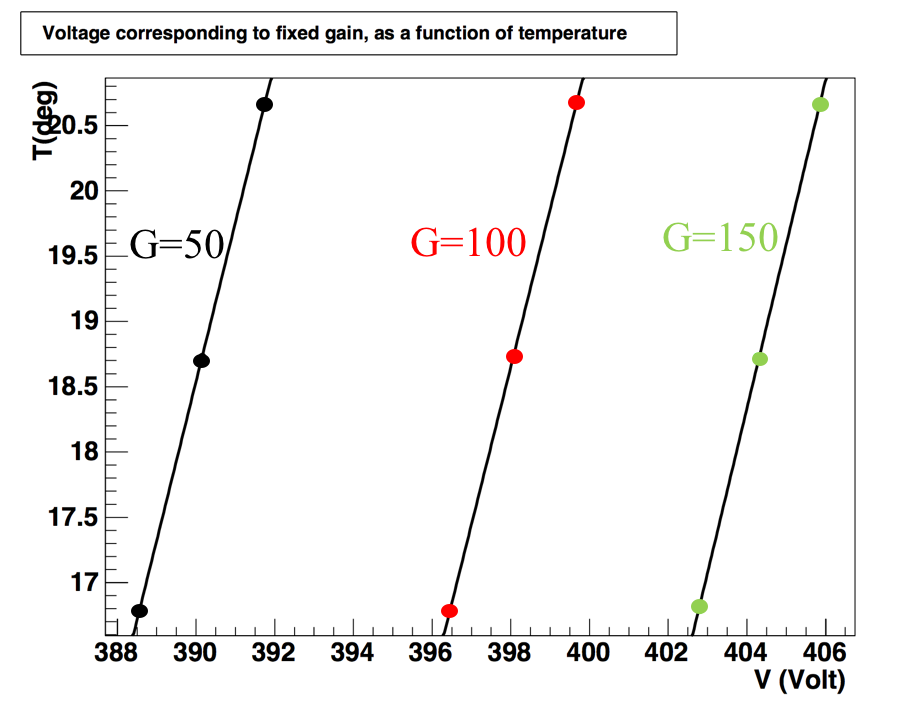
\includegraphics[width=0.5\textwidth]{pics/experiment/apdTV.png}
  \caption[APD fixed gain in terms of voltage and temperature]{The calculated voltages for fixed gains as a function of temperature can be used to group the APDs for common high voltage.}
  \label{Figure:apdTV}
\end{figure}


\section{Trigger}
Events of interest in the HPS experiment are triggered by the ECal. Each channel of the ECal is readout to an FADC250 with 16 channels per board. The FADC250 continuously samples analog signals at a rate of 250~MHz, or every 4~ns with 12-bit precision. As the data size was small enough, the 2015 and 2016 data was recorded in raw mode such that 100~samples of raw information in a channel are read at the trigger time. This raw mode, called Mode 1, allowed for precise offline pulse fitting of the signals for optimal energy resolution and improved timing resolution.\\
\indent When a signal crosses a pre-defined threshold, a set number of samples before and after the crossing are summed together to provide a pulse charge value which is converted to energy. The conversion to energy requires access to the individual channel gains and pedestals (as found by cosmic calibrations) which are pre-loaded into the data acquisition (DAQ) system. The energy and time of threshold crossing are sent to the General Trigger Processor (GTP) board every 16~ns  for clustering.~\cite{balossino_hps_2016}\\
\indent The GTP clusterer first identifies the crystal carrying the highest energy (known as the seed hit) in comparison to all surrounding crystals. The immediately neighboring crystals of the seed hit are compared in both energy and time coincidence with respect to the seed crystal in order to create a cluster. The cluster energy is the sum of all of the hits in a cluster. The timing coincidence is typically chosen to be 4~samples to allow for time-walk effects. The cluster information is then passed to the Subsystem Processor (SSP) to make a trigger decision based on various settable trigger cut requirements. \\
\indent The SSP includes several different configurations that can run simultaneously containing different settable cuts and prescale values for ECal modules. The SSP looks for combinations of clusters that pass the configuration requirements and cuts and then sends a trigger to the Trigger Supervisor (TS) board when a cluster or pair of clusters satisfies the trigger requirements. The trigger is then sent to the Trigger Interface (TI) boards in order to trigger readout of all detectors.\\ 
\indent The SSP trigger configurations include two cluster pairs triggers, two single cluster triggers, a random pulser trigger, a cosmic trigger, and an LED trigger of which all except for the cosmic and LED trigger were run during data taking with beam. The single cluster trigger, Single-1, was optimized for elastically-scattered beam energy electrons off the target. The looser version of the trigger was Single-0. These triggers were useful in selecting events for calibrating the ECal and studying the trigger efficiencies. The cluster pairs trigger is the primary trigger for the HPS experiment and studies all possible combinations of clusters in the ECal for pairs selection. The tuneable cuts used in this trigger are presented in Table~\ref{tab:pairTriggerCuts}.~\cite{balossino_hps_2016} 

\begin{table}[H]
\caption{Pair-1 Trigger Cuts}
\label{tab:pairTriggerCuts}
\centering
\begin{tabular}{lc}
\toprule
%\multicolumn{2}{c}{Name} \\
%\cmidrule(r){1-2}
Trigger cut & Cut value \\
\midrule
Time difference & $| t_{top}-t_{bot} | \leq t_{coincidence}$   \\
Cluster energy & $E_{min}<E_{i}<E_{max}$\\
Cluster sum & $E_{sum min}\leq E_1+E_2\leq E_{sum max}$\\
Cluster size & $N_{hits}\geq N_{threshold}$\\
Energy difference & $ E_{2}-E_{1}<E_{difference}$\\
Coplanarity & $ |\arctan\dfrac{x_1}{y_1}-\arctan\dfrac{x_2}{y_2} | \leq \theta_{coplanarity}$\\
Energy-distance & $E_{1}+r_{1}F\geq E_{slope}$ \\ 
\bottomrule
\end{tabular}
\end{table}

In Table~\ref{tab:pairTriggerCuts}, the variables $t_i,E_i, N_i, x_i,$ and $y_i$ denote the cluster time, cluster energy, number of hits in the cluster, and coordinates of the cluster, respectively. The subscript, $1$, denotes the cluster with the lowest energy of the pair.  The parameter, $r_1$, is the distance between the center of the lowest energy cluster and the center of the ECal (defined as $r_1=\sqrt{x_1^2+y_1^2}$). The parameters selected for the cuts include the $t_{coincidence}, E_{min}, E_{max}, E_{sum min}, E_{sum max}, N_{threshold}, E_{difference}, \theta_{coplanarity}, r_{1},$ and $E_{slope}$, and are chosen from studying A$^{\prime}$ Monte Carlo in order to optimize the signal acceptance while minimizing the background. The GTP clusters are created prior to track-matching and offline clustering (which includes hits belonging to a cluster beyond those immediately adjacent to the seed hit). For the 2015 data, a GTP cluster conserves roughly 80$\%$ of the fully reconstructed particle energy when the seed hit is not on the edge of the ECal. \\
\indent The time coincidence cut is kept loose enough in the SSP pairs cluster selection to allow for time walk and cabling offsets which are not corrected for until the full pulse is fitted in offline reconstruction. At the GTP stage, the time only corresponds to threshold crossing. The cluster energy cut is inclusive of clusters that are reconstructed by the GTP in the energy range of interest. The minimum hit requirement for clusters was lowered at the start of running due to A$^{\prime}$ Monte Carlo studies indicating that 1 hit clusters were possible and could improve reach without overburdening the trigger. The cluster sum cut most significantly removes accidental pairs containing elastically-scattered beam energy electrons in addition to removing low energy cluster sum events that will not pass thresholds for well-reconstructed events. The energy difference cut removes events that have extremely different cluster energies and do not satisfy $A^{\prime}$-type criteria. \\
\indent The coplanarity cut removes events that are not coplanar including M$\o$ller and wide-angle bremsstrahlung (WAB) backgrounds because the $e^+e^-$ trident events of interest are distributed symmetrically around the beamline. The angle is calculated from the center of the ECal where the beam line passes through to each cluster in the pair relative to the vertical axis. The pairs should be approximately $180\degree$ apart. \\
\indent The energy-distance cut is applied to the lowest-energy cluster of the pair in order to reject events where the cluster is too close to where the electron beam passes through the ECal. Trident kinematics show that most of these clusters are dominated by bremsstrahlung low energy photons and that there is some reasonable distance of separation with respect to the beamline for these lower energy events. 
\indent The cut values used in the 2015 Pair-1 trigger are shown in Table~\ref{tab:pairTriggerVals}.

\begin{table}[H]
\caption{Pair-1 trigger cut values for the Engineering Run}
\label{tab:pairTriggerVals}
\centering
\begin{tabular}{lc}
\toprule
%\multicolumn{2}{c}{Name} \\
%\cmidrule(r){1-2}
Trigger cut & Cut value \\
\midrule
Time difference & $| t_{top}-t_{bot} | \leq12$ ns   \\
Cluster energy & $54<E<630$ MeV \\
Cluster size & $N_{hits}\geq 1$\\
Energy sum & $180<E_{top}+E_{bot}<860$ MeV\\
Energy difference & $| E_{top}-E_{bot}|<540$ MeV\\
Coplanarity & $\theta_{top}-\theta_{bot}<30\degree $\\
Energy-distance & $E_{1}+(5.5 MeV/mm)r_{1}>600$ MeV\\ 
\bottomrule
\end{tabular}
\end{table}

\indent The pulser trigger generates a constant rate of triggers at 100~Hz regardless of the physics events as measured by the ECal. This makes the pulser an unbiased probe for measuring the backgrounds of the experiment during running with the beam and concurrent with other triggers.\\ 
\indent The cosmic trigger was used without the beam for calibration of the ECal and uses the timing coincidence between two scintillators, placed below and external to the ECal, in order to trigger readout of all ECal channels for offline reconstruction of the cosmic event. The timing coincidence of the scintillators placed in line and below the ECal was chosen to be 40~ns where the leading edge of the scintillator signal in the FADC pulse crosses 60~ADC. Once the timing and threshold conditions are met, all modules in the ECal were readout in Mode 1 format. 


%%%%%%%%%%%%%%%%%%%%%%%%%%%%%%%%%%%%%%%%%
\chapter{Detector Calibration and Performance} 
The first detector to be commissioned was the ECal during preliminary running with a 2~GeV electron beam in Hall B in December 2014. The ECal was initially calibrated prior to receiving any beam using cosmic ray energy deposition in the crystals. The ECal demonstrated that all channels worked and that the full readout chain using FADC250 modules with the DAQ performed well. The SVT was installed in the early spring of 2015 and was fully commissioned during the Engineering Run. The single pass beam energy was 1.056~GeV and was sufficient for detector commissioning, calibration, and physics analysis. 

\section{Silicon Vertex Tracker Performance}
The SVT momentum calibration is primarily guided by the accuracy of the alignment in the magnetic field. Tracks on both top and bottom for elastically-scattered electrons should peak at the same beam energy at the same resolution. The Billoir vertexing algorithm is the method by which two tracks are re-fit to create a vertex. The invariant mass is reconstructed from the vertex of the two tracks. 

%\subsection{M\o ller mass}

\subsection{Momentum resolution}


\subsection{Tracking efficiency}

(Include discussion on layer efficiency, 3 prong tracking efficiencies, moller mass, and fee peak resolution.)

\section{Electromagnetic Calorimeter}
The ECal was calibrated both in energy and time. The first calibration performed before receiving beam from the accelerator was the cosmic ray energy calibration. A full timing calibration of the ECal was also performed using the accelerator RF signal. A final calibration using physics events from elastically-scattered beam energy electrons and events from wide angle bremsstrahlung (WAB) yielded the full calibration of the ECal for all energies and characterized the energy resolution. 

\subsection{Simulations}
The ECal uses an adapted version of the clustering algorithm that was used by the CLAS IC. The geometrical arrangement of the crystals differs greatly from that used by the IC and required detailed studies and simulations to reconstruct the incident particle energy. The angles of incidence of the particles (electrons, positrons, and photons) entering the Ecal varies significantly across the ECal. The edge effects in the ECal are substantial due to the horizontal split between the top and bottom halves and  the proximity to the beam. \\
\indent Simulations were performed using the fully modeled detector geometry in SLIC as part of the standard hps software package. The geometry includes all strips of the SVT, vacuum chambers, ECal crystals, and relevant dead material. The geometry also moves particles through a 3D magnetic field map corresponding to the field values for 1~GeV beam running.~\cite{CalibNote} \\
\indent Single particles: electrons, positrons, and photons were simulated at discrete energies of 0.2, 0.3, 0.4, 0.5, 0.6, 0.7, 0.8,  0.9, 1.0, and 1.1~GeV to uniformly cover the ranger of energies detectable in the Engineering Run. The simulation uses the full reconstruction chain excluding pile-up effects. The offline cluster reconstruction uses the same thresholds used in data and production Monte Carlo: 7.5~MeV for individual hits, 50~MeV for seed hits in clusters, and 100~MeV for cluster energies.\\

\subsubsection{Energy reconstruction}
\indent Due to the complex showering cascade that occurs when a particle deposits its energy in the ECal, several adjacent crystal modules contain some fraction of the incident energy of the particle. These modules are clustered in offline reconstruction to obtain the total deposited energy of the incident particle. The reconstructed energy not corrected for shower loss effects is defined by Equation~\eqref{eq:eclsum}.

\begin{equation}
\label{eq:eclsum}
E_{rec} = \sum_i E_i    
\end{equation}

In Equation~\eqref{eq:eclsum}, the subscript $i$ pertains to each module in the cluster such that $E_i$ is the energy of each module in the cluster. Some incident particle energy is lost between crystals and out the back where the APD does not fully cover the surface of each crystal. After recovering the energy as measured by the ECal, the incident particle energy can be found by correcting for the shower loss effects as described by Equation~\eqref{eq:eclsf}.

\begin{equation}
\label{eq:eclsf}
E_{corr} = \dfrac{E_{rec}}{f}   
\end{equation}

In Equation~\eqref{eq:eclsf}, $f$ is the energy-dependent ratio of measured vs incident particle energy. This factor is obtained through simulation. The energy loss corrections as derived from Monte Carlo are shown in Fig.~\ref{Figure:ecorr} where $E_{gen}$ refers to the simulated Monte Carlo particle energy.

\begin{figure}[thb]
  \centering
      \includegraphics[width=0.75\textwidth]{pics/performance/energycorrection.pdf}
  \caption[ECal energy shower correction functions from simulation]{Energy correction functions correct the energy measured in the ECal to reconstruct the energy of the incident particle.}
  \label{Figure:ecorr}
\end{figure}

The difference in the energy corrections for the various particle types arises from geometrical effects and the incident angles of the particles entering the crystals.~\cite{Garcon} The focal point of the calorimeter, the point at which all crystals are angles, lies 80~cm from the front face of the ECal. The HPS target is beyond this focal distance at approximately 1.3~m from the face of the ECal and is offset beam right in the pair spectrometer magnetic field. Particles produced at the target take different trajectories from the target to the ECal due to the interactions of their charge and momentum in the magnetic field. This affects the entry angle of the particle into a crystal and mandates a charge and momentum-dependent energy correction function. The form of the energy correction function for the central region of the ECal is described by a three parameter fit in Eq.~\eqref{eq:ecorrfunc}.

\begin{equation}
	\label{eq:ecorrfunc}
	\dfrac{E_{rec}}{E_{gen}} = \dfrac{A}{E_{rec}}+\dfrac{B}{\sqrt{E_{rec}}}+C 
\end{equation}

The shower leakage effects in crystals becomes significant at distances close to the edge. The energy reconstruction deteriorates rapidly in the crystals closest to the edge but stabilizes in central region of the ECal. The energy reconstruction at the edges was fully characterized using Monte Carlo as a function of position in the ECal relative to the inner beam gap edge. In Equation ~\eqref{eq:ecorrfunc}, parameter $A$ is not strongly correlated with position and remains as a constant for a given particle type. The parameters $B$ and $C$  do depend on cluster position relative to the beam gap edge of the ECal. These dependencies can be seen for electrons in Fig.~\ref{Figure:sfparEdge}.

\begin{figure}[H]
  \centering
      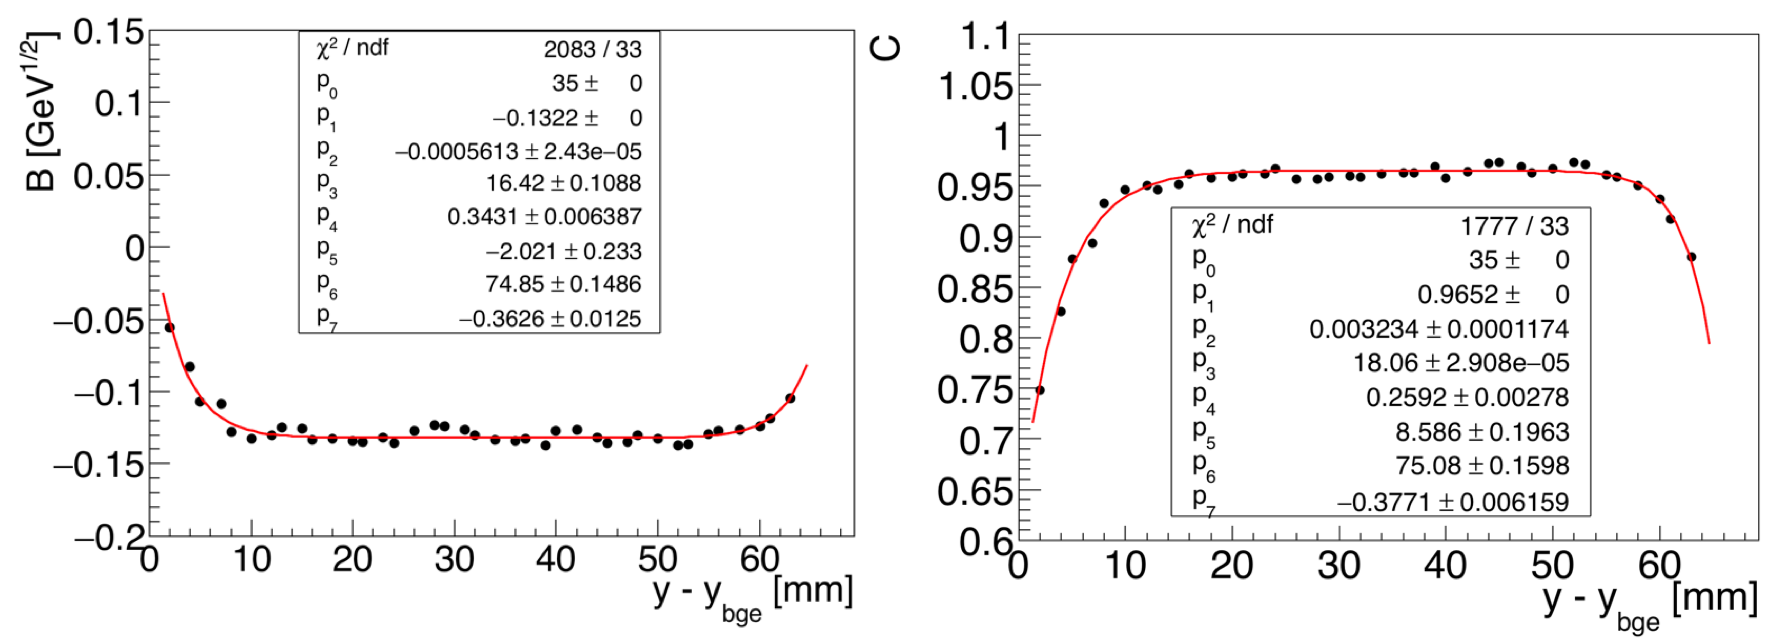
\includegraphics[width=1.0\textwidth]{pics/performance/sfparEdgeFit.png}
  \caption[ECal energy shower parameters for electrons relative to the inside beam gap edge]{Parameters $B$ and $C$ from Eq.~\ref{eq:ecorrfunc} for electrons, as a function of vertical position
relative to the innermost beam gap edge.}
  \label{Figure:sfparEdge}
\end{figure}

As shown in Fig.~\ref{Figure:sfparEdge}, the energy leakage parameters $B$ and $C$ can be fit with two functions at the edges that match in the central region of the ECal, away from the edges of the calorimeter. The equations used to fit the $B$ and $C$ parameters are described by Equations ~\eqref{eq:p1parlt} and ~\eqref{eq:p2parlt}, respectively.

\begin{equation}
\begin{split}
\label{eq:p1parlt}
B(y<p_0) = p_1-p_2 e^{-(y-p_3)p_4}\\
B(y>p_0) = p_1-p_5 e^{-(y-p_6)p_7}
\end{split}
\end{equation}

\begin{equation}
\begin{split}
\label{eq:p2parlt}
C(y<p_0) = p_1-p_2 e^{-(y-p_3)p_4}\\
C(y>p_0) = p_1-p_5 e^{-(y-p_6)p_7}
\end{split}
\end{equation}

The energy leakage correction functions are relatively constant in the central region of the calorimeter and are matched at a central distance $p_0$. For columns containing 5 crystals vertically, the distance to the beam gap edge is the absolute value of the distance from the cluster centroid to the innermost beam gap edge. In the regions above and below the region where row 1 crystals are removed in the ECal, additional consideration is made when calculating the distance to the inner beam gap edge in order to be consistent with other regions of the ECal. For completeness, the corresponding energy correction parameters for positrons and photons are seen in Figures~\ref{Figure:sfparEdgeEP} and \ref{Figure:sfparEdgeP}, respectively. 


\begin{figure}[H]
  \centering
      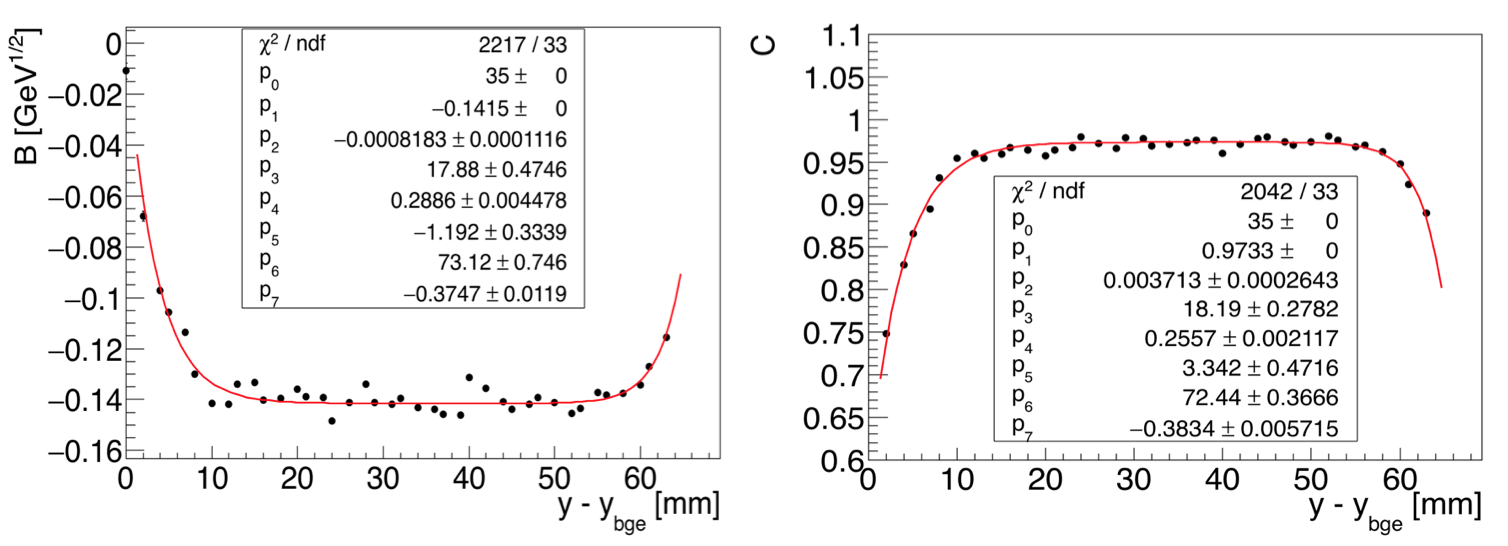
\includegraphics[width=1.0\textwidth]{pics/performance/sfparEdge_ep.png}
  \caption[ECal energy shower parameters for positrons relative to the inside beam gap edge]{Parameters $B$ and $C$ from Eq.~\ref{eq:ecorrfunc} for positrons, as a function of vertical position
relative to the innermost beam gap edge.}
  \label{Figure:sfparEdgeEP}
\end{figure}

\begin{figure}[H]
  \centering
      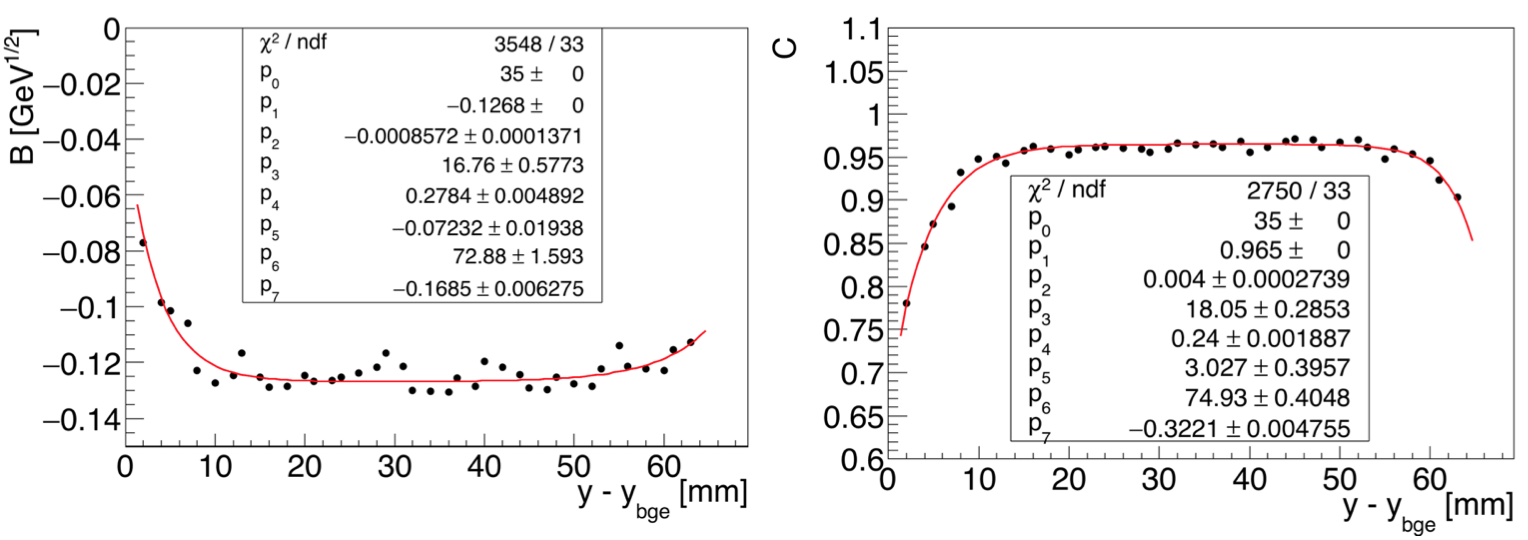
\includegraphics[width=1.0\textwidth]{pics/performance/sfparEdge_p.png}
  \caption[ECal energy shower parameters for photons relative to the inside beam gap edge]{Parameters $B$ and $C$ from Eq.~\ref{eq:ecorrfunc} for photons, as a function of vertical position
relative to the innermost beam gap edge.}
  \label{Figure:sfparEdgeP}
\end{figure}

As one can see, the energy corrections are relatively constant at approximately 1~cm from the edges of the ECal. As a result, we define the fiducial the region of the ECal to be at greater than 1~cm from the edge, or approximately 3/4 of the font face crystal dimension. This result is consistent with the findings for the CLAS IC.~\cite{Garcon} 

\subsubsection{Energy resolution}

The energy resolution of the ECal is energy-dependent and improves with energy as $1/\sqrt{E}$. From simulation, we obtain the energy resolution as shown in Figure~\ref{Figure:eResFitMC}.

\begin{figure}[H]
  \centering
      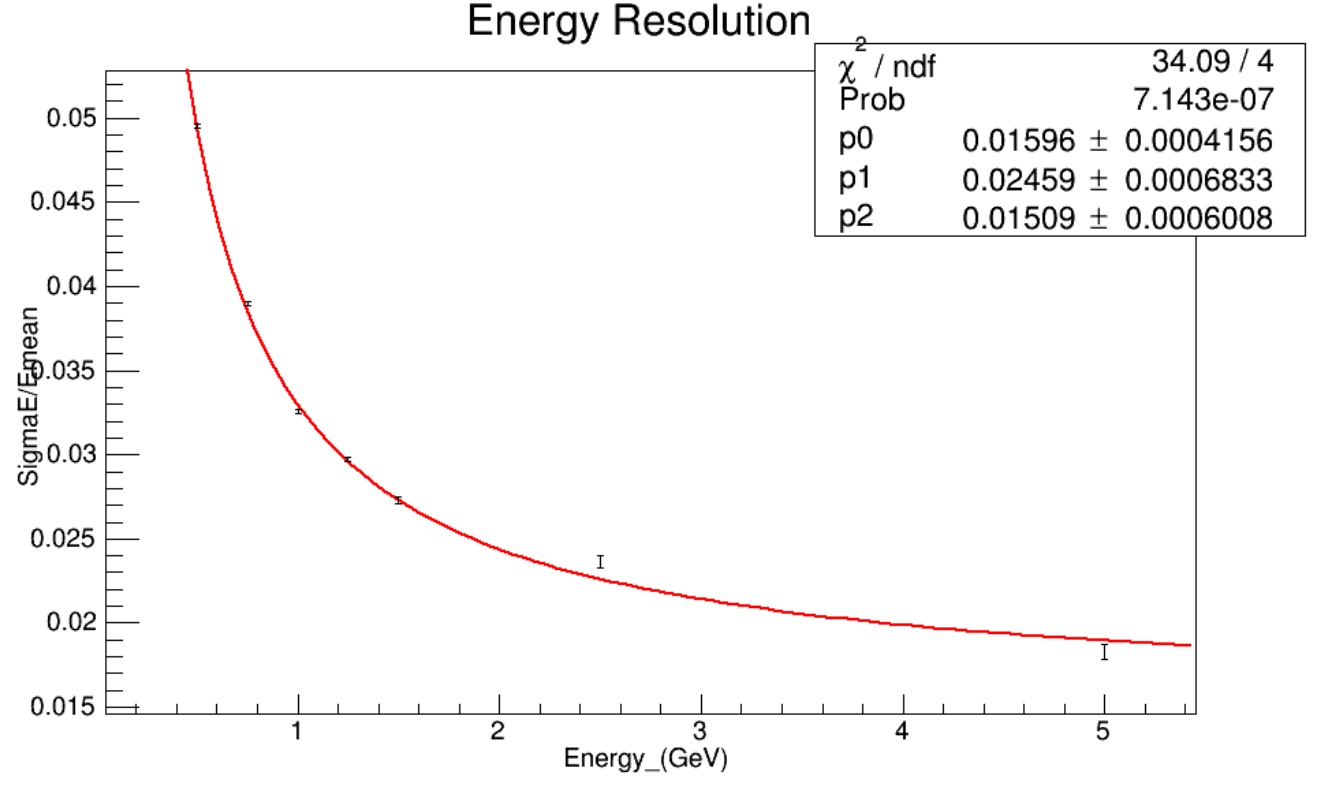
\includegraphics[width=0.6\textwidth]{pics/performance/eResFitMC.png}
  \caption[ECal energy resolution fitted from simulation]{ECal energy resolution from simulation.}
  \label{Figure:eResFitMC}
\end{figure}

The fit shown in Figure~\ref{Figure:eResFitMC} is described by Equation~\ref{eq:eResMC}.

\begin{equation}
\label{eq:eResMC}
\dfrac{\sigma_E}{E} (\%) = \dfrac{1.60}{E} \oplus \dfrac{2.46}{\sqrt{E}} \oplus 1.51
\end{equation}

The first term corresponds to the preamplifier noise. We were expecting 3~MeV$\times \sqrt{10} = 0.009$~GeV, where 10 is the average number of hit crystals. This term from simulation is not including the FADC error (expected to be 1.3~MeV~\cite{Charles}) which contributes a term (in $\%$) as $0.13\sqrt{10}/E$ to be added, quadratically. The second term corresponds to the statistical fluctuations in the shower development and is influenced by the lateral containment of the shower and energy deposited in the crystal module. The second term from simulation is not including fluctuations in the number of photoelectrons (30 photoelectrons/MeV, multiplied by an excess noise factor parameterizing the fluctuations in the APD gain process, or Fano factor, of 2~\cite{panda}) contributing $0.8/\sqrt{E}$. This term is calculated as $\sqrt{F/N_{pe/GeV}}$. The third term is interpreted as the fluctuation of energy leakage through the back of the crystals. This third term should includ the crystal-to crystal inter-calibration error which estimate to be 1~$\%$.~\cite{Garcon} By including these additional resolution effects in the measurement, we obtain the resolution as anticipated from Monte Carlo in Equation~\eqref{eq:eResUpdated}.

\begin{equation}
\label{eq:eResUpdated}
\dfrac{\sigma_E}{E} (\%) = \dfrac{1.65}{E} \oplus \dfrac{2.59}{\sqrt{E}} \oplus 1.81 
\end{equation}

\subsubsection{Position reconstruction}
\indent ECal clusters provide position information of comparable resolution to the SVT. Various weighting schemes for calculating a cluster centroid can be problematic due to periodic patterns resulting from the segmentation of the crystals. The same weighting scheme, used by the CLAS IC algorithm, provided the optimal position resolution. The calculation of the position of the cluster is shown in Equation~\eqref{eq:posncalc}.~\cite{Garcon}

\begin{eqnarray*}
\label{eq:posncalc}
x_{cl} & = & \dfrac{\sum_i w_i x_i}{\sum_i w_i}\\
y_{cl} & = & \dfrac{\sum_i w_i y_i}{\sum_i w_i}\\
\end{eqnarray*}

In Equation~\eqref{eq:posnwt}, the index $i$ indicates the individual module in the cluster, and $w_i$ is described by Equation~\eqref{eq:posnwt}.

\begin{equation}
\label{eq:posnwt}
w_i  =  max[0, w_0+ ln\dfrac{E_i}{E_{rec}}]
\end{equation}

The parameter $w_0$ in Equation~\eqref{eq:posnwt} is an energy threshold such that $E_i/E_{cl} > e^{-w_0}$ and is found in simulation to have a value of $3.1$ \cite{Garcon}. The logarithmic term enhances the contribution from the tails and improves the position measurement. Additional effects resulting from the differing angles of entry at the ECal require a position correction to the $x$-coordinate of the cluster. These corrections are both charge and momentum-dependent. The position correction for a generated 1~GeV electron is shown in Figure~\ref{Figure:xposn1gev}.

\begin{figure}[H]
  \centering
      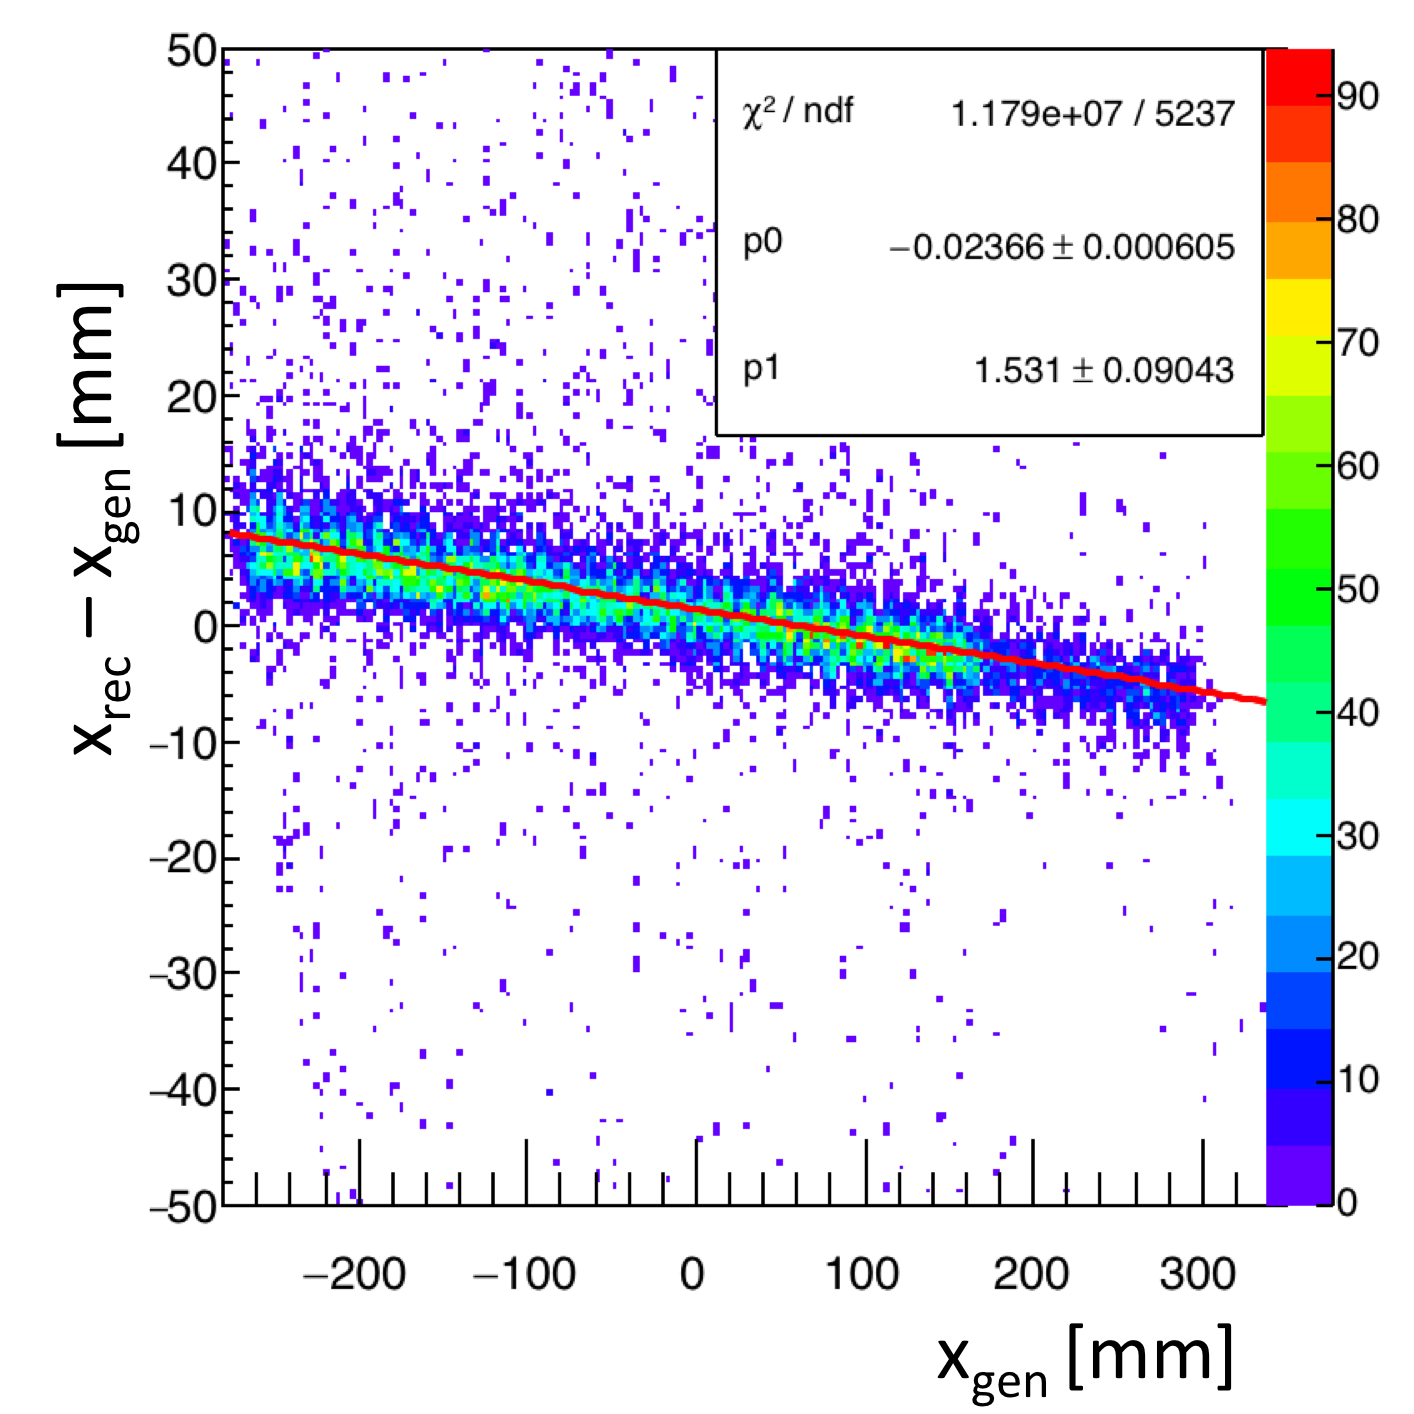
\includegraphics[width=0.7\textwidth]{pics/performance/xposn1gev.png}
  \caption[Horizontal position correction for 1~GeV electrons]{The position correction as found for a 1~GeV electron is both energy and position-dependent in order to account for the different angle of incidence at the ECal.}
  \label{Figure:xposn1gev}
\end{figure}

The correction at each energy by particle-type is fit with Equation~\eqref{eq:posncorr}. 

\begin{equation}
\label{eq:posncorr}
x_{rec} - x_{gen} = A(E_{rec}) x_{gen} + B(E_{rec})
\end{equation}

The energy-dependence of the fit parameters $A(E_{rec})$ and $B(E_{rec})$ use the reconstructed cluster energy, uncorrected for shower loss effects. These parameters for the electron horizontal position correction as a function of the reconstructed cluster energy are shown Figure~\ref{Figure:xposcorrPar}.

\begin{figure}[H]
  \centering
      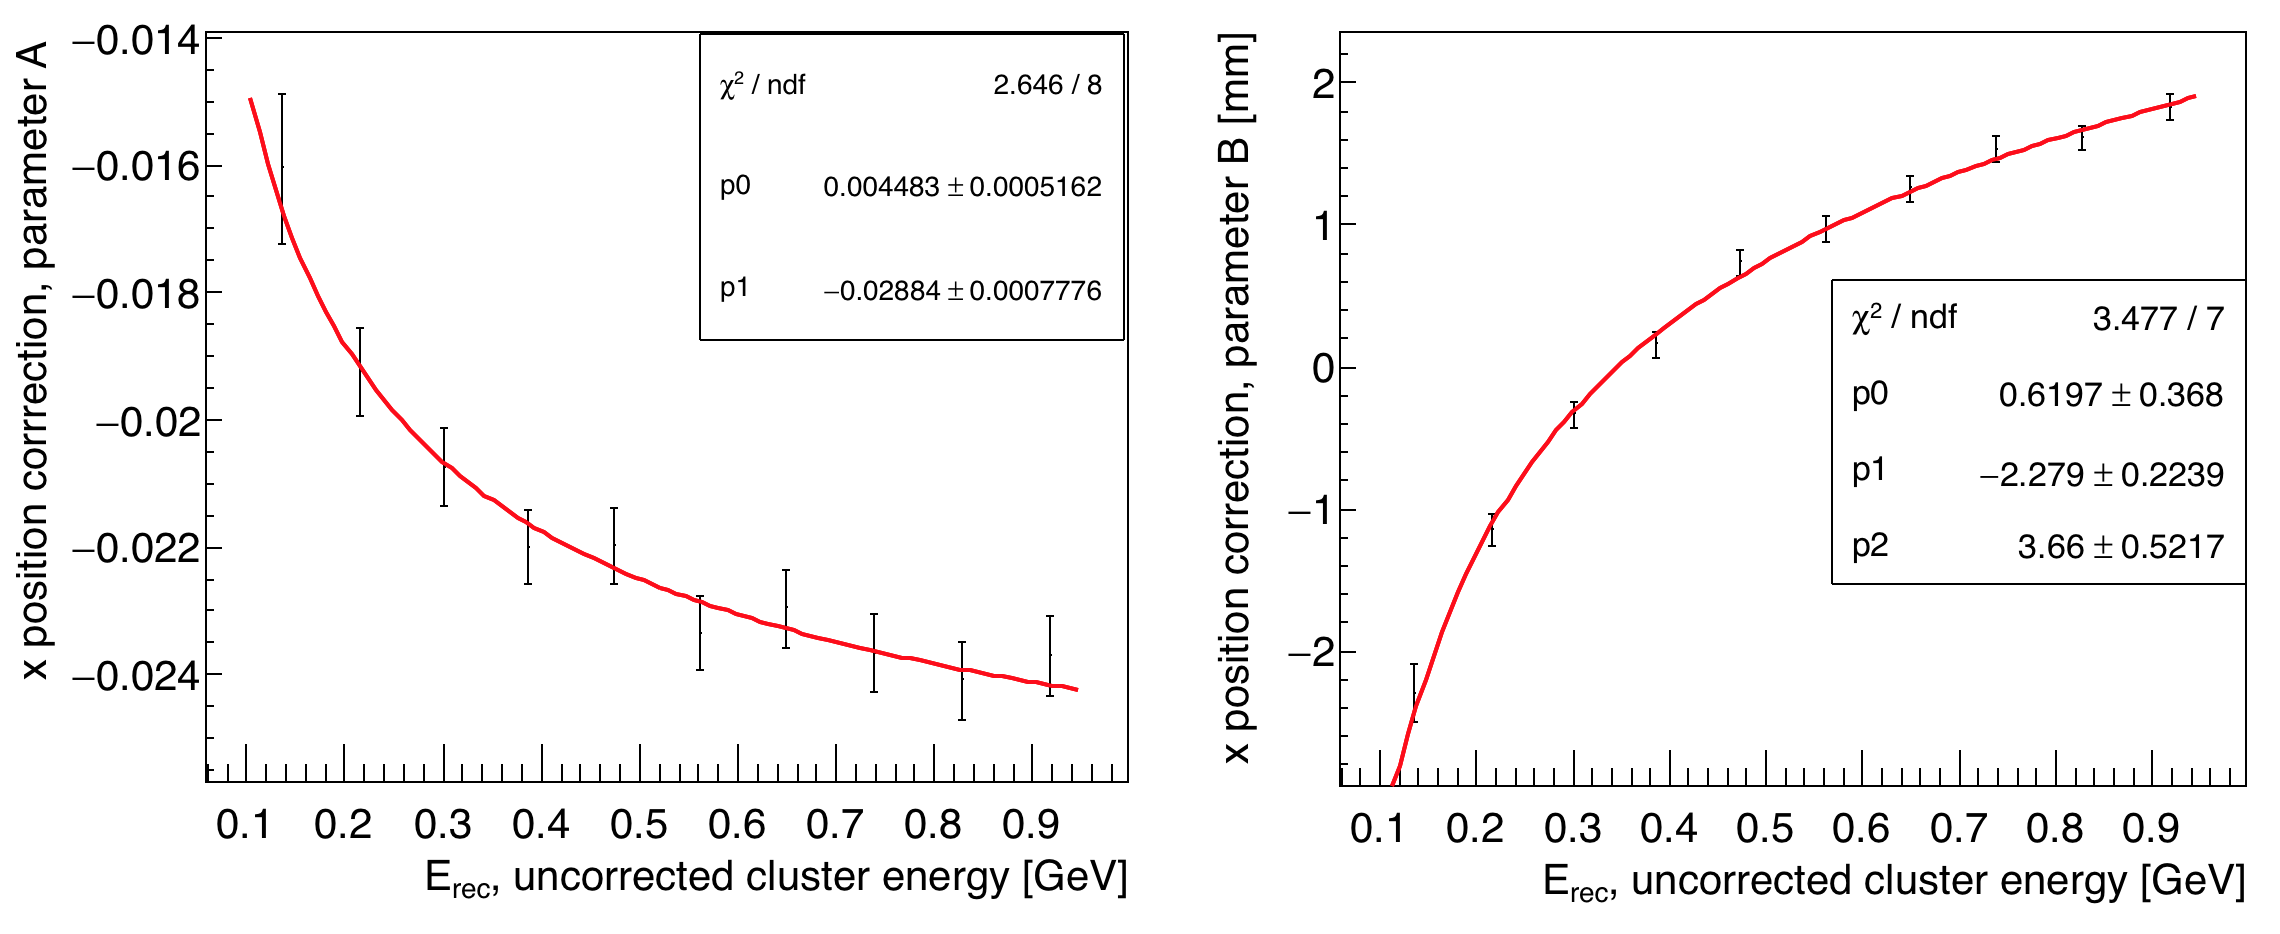
\includegraphics[width=1.0\textwidth]{pics/performance/xposcorrPar.png}
  \caption[Horizontal position correction dependence for electrons]{The horizontal position correction parameters as functions of the uncorrected cluster energy.}
  \label{Figure:xposcorrPar}
\end{figure}

The parameters in Figure~\ref{Figure:xposcorrPar} are fit to functions of the form described in Equation~\eqref{eq:posnCpar}.

\begin{eqnarray*}
\label{eq:posnCpar}
A(E_{rec}) & = & \dfrac{p0}{\sqrt{E_{rec}}}+p1\\
B(E_{rec}) & = & p0\times E_{rec} +\dfrac{p1}{\sqrt{E_{rec}}}+p2
\end{eqnarray*}

The corresponding correction values for all three particle types can be summarized in Table~\ref{tab:horizPosCorr}.

\begin{table}[H]
\caption{Horizontal position corrections.}
\label{tab:horizPosCorr}
\centering
\begin{tabular}{|c|c|c|}
\toprule
%\multicolumn{2}{c}{Name} \\
%\cmidrule(r){1-2}
Particle & $A(E_{rec})$ & $B(E_{rec})$ \\
\midrule
electron & $0.004483/\sqrt{E_{rec}}-0.02884$ & $0.6197E_{rec}-2.279/\sqrt{E_{rec}}+3.66$ \\
positron & $0.006887/\sqrt{E_{rec}}-0.03207$ & $-0.8048E_{rec}+0.9366/\sqrt{E_{rec}}+2.628$ \\
photon & $0.005385/\sqrt{E_{rec}}-0.03562$ & $-0.1948E_{rec}-0.7991/\sqrt{E_{rec}}+3.797$ \\
\bottomrule
\end{tabular}
\end{table}

Position corrections are not needed for the vertical cluster position.

\subsubsection{Position resolution}

After applying the position corrections to each particle-type at the simulated energies, the residual between the measured and simulated position reconstruction is obtained is measured. The fitted residuals after correcting the position of 1~GeV electron clusters are shown in Figure~\ref{Figure:corrPosnsFits}.

\begin{figure}[H]
  \centering
      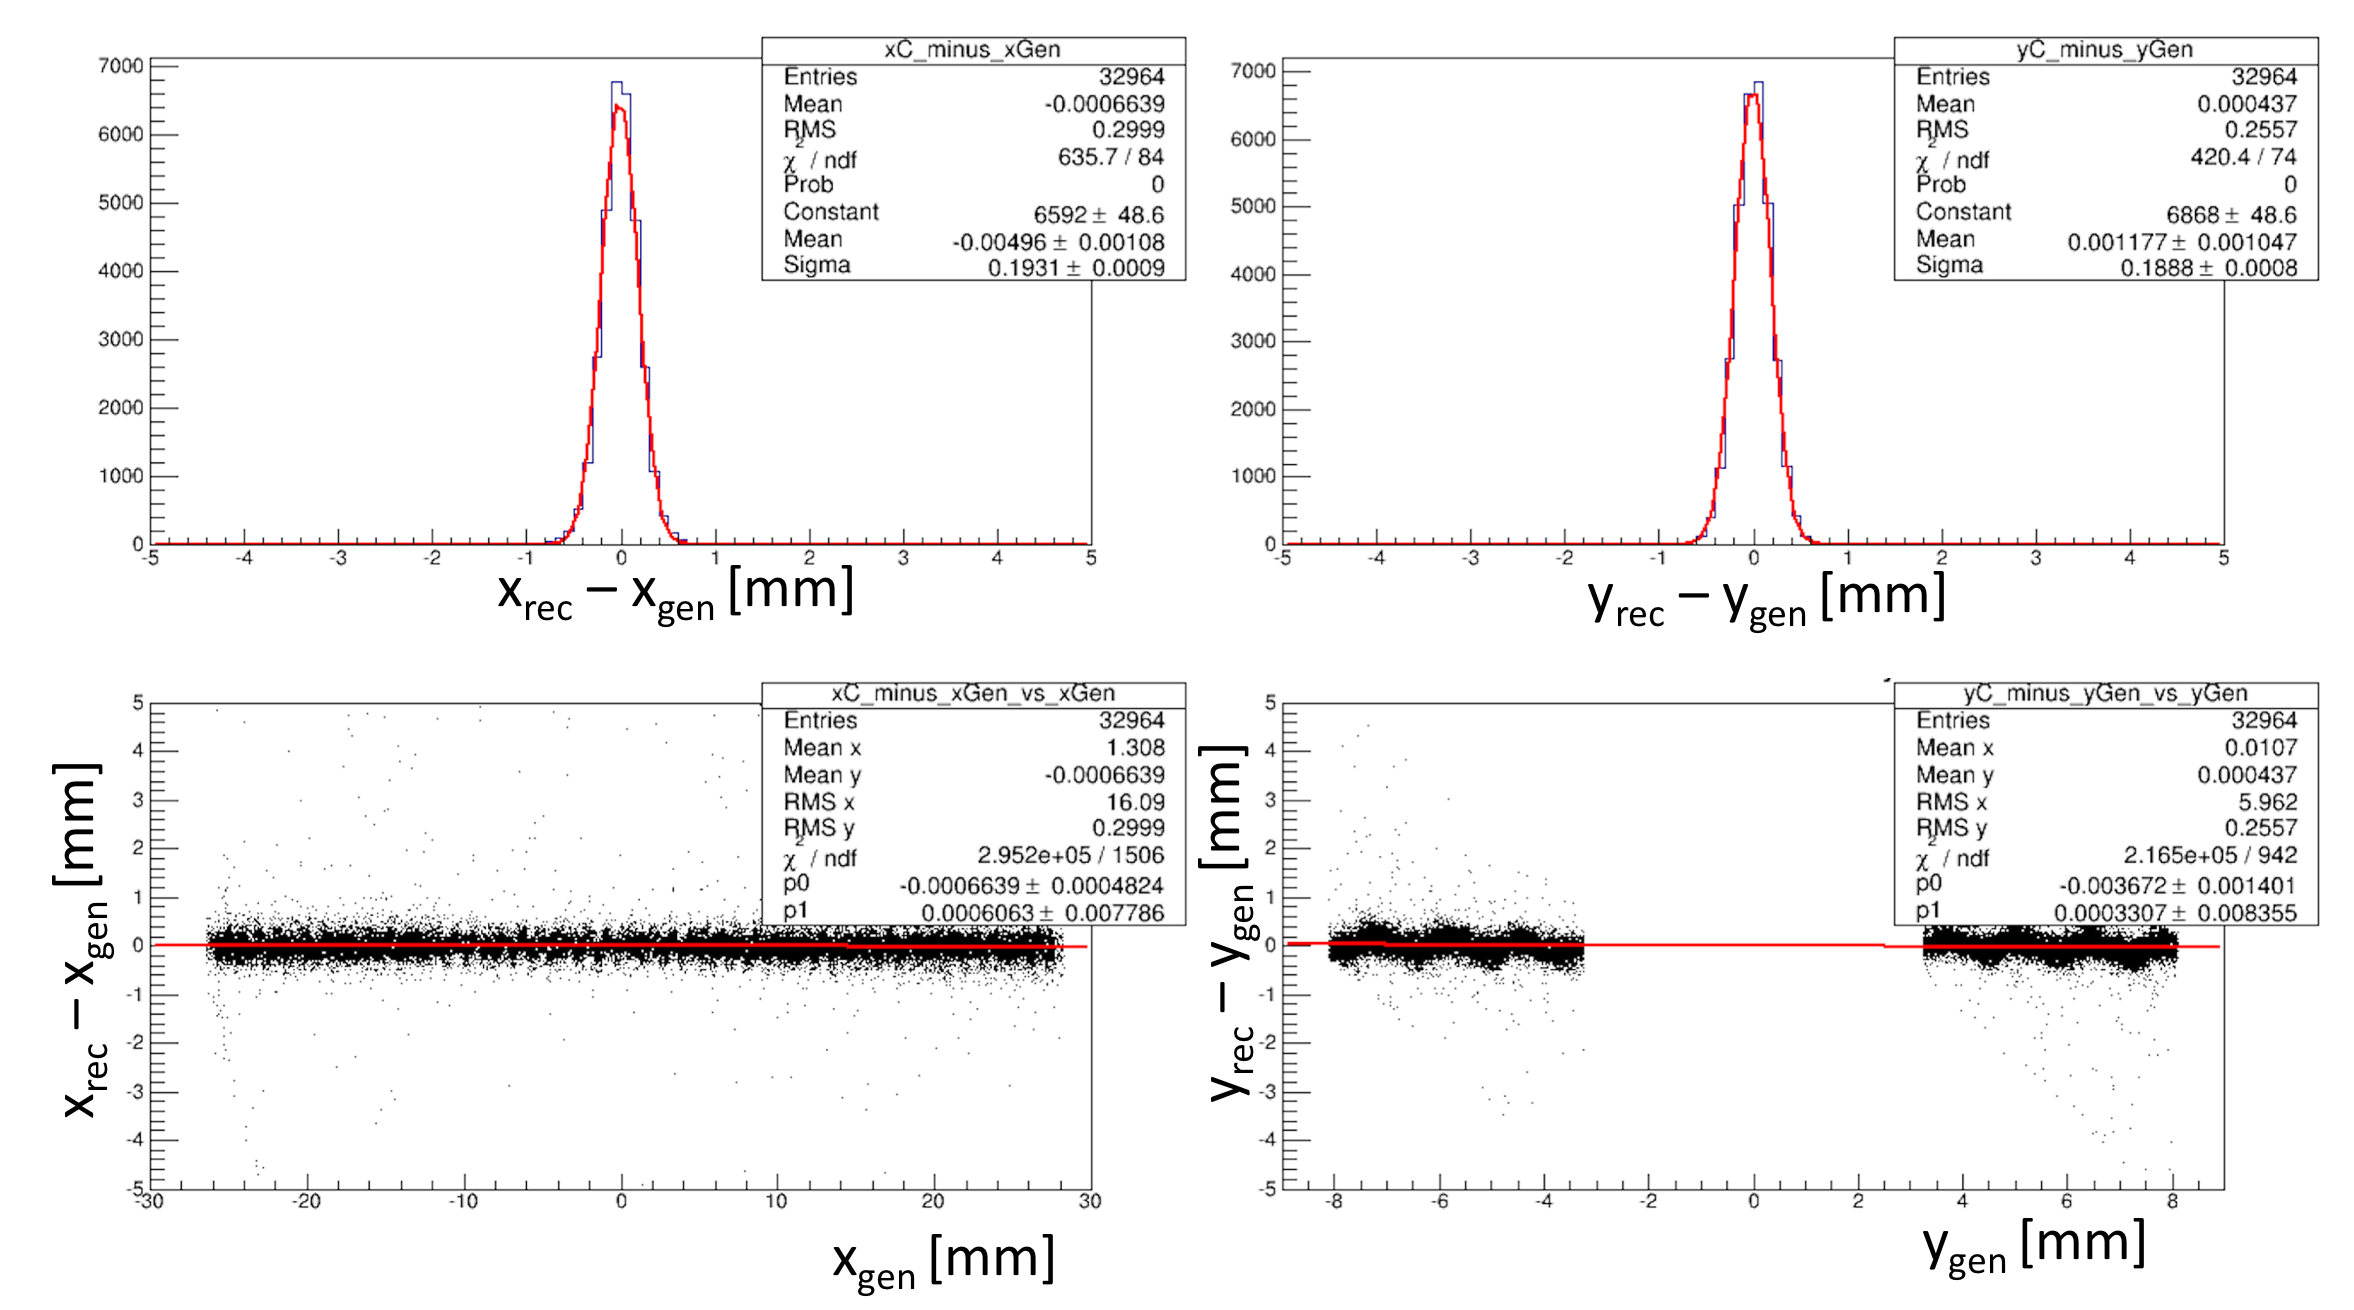
\includegraphics[width=1.0\textwidth]{pics/performance/corrPosnsFits.png}
  \caption[Position resolution for 1~GeV electrons.]{The position resolution for 1~GeV electrons, after applying the horizontal position corrections.}
  \label{Figure:corrPosnsFits}
\end{figure}

As shown in Figure~\ref{Figure:corrPosnsFits}, no correction is required when reconstructing the vertical position of the cluster. The energy-dependent resolution of both the horizontal and vertical position of reconstructed clusters can be seen for electrons in Figure~\ref{Figure:emPosnResn}. 

\begin{figure}[H]
  \centering
      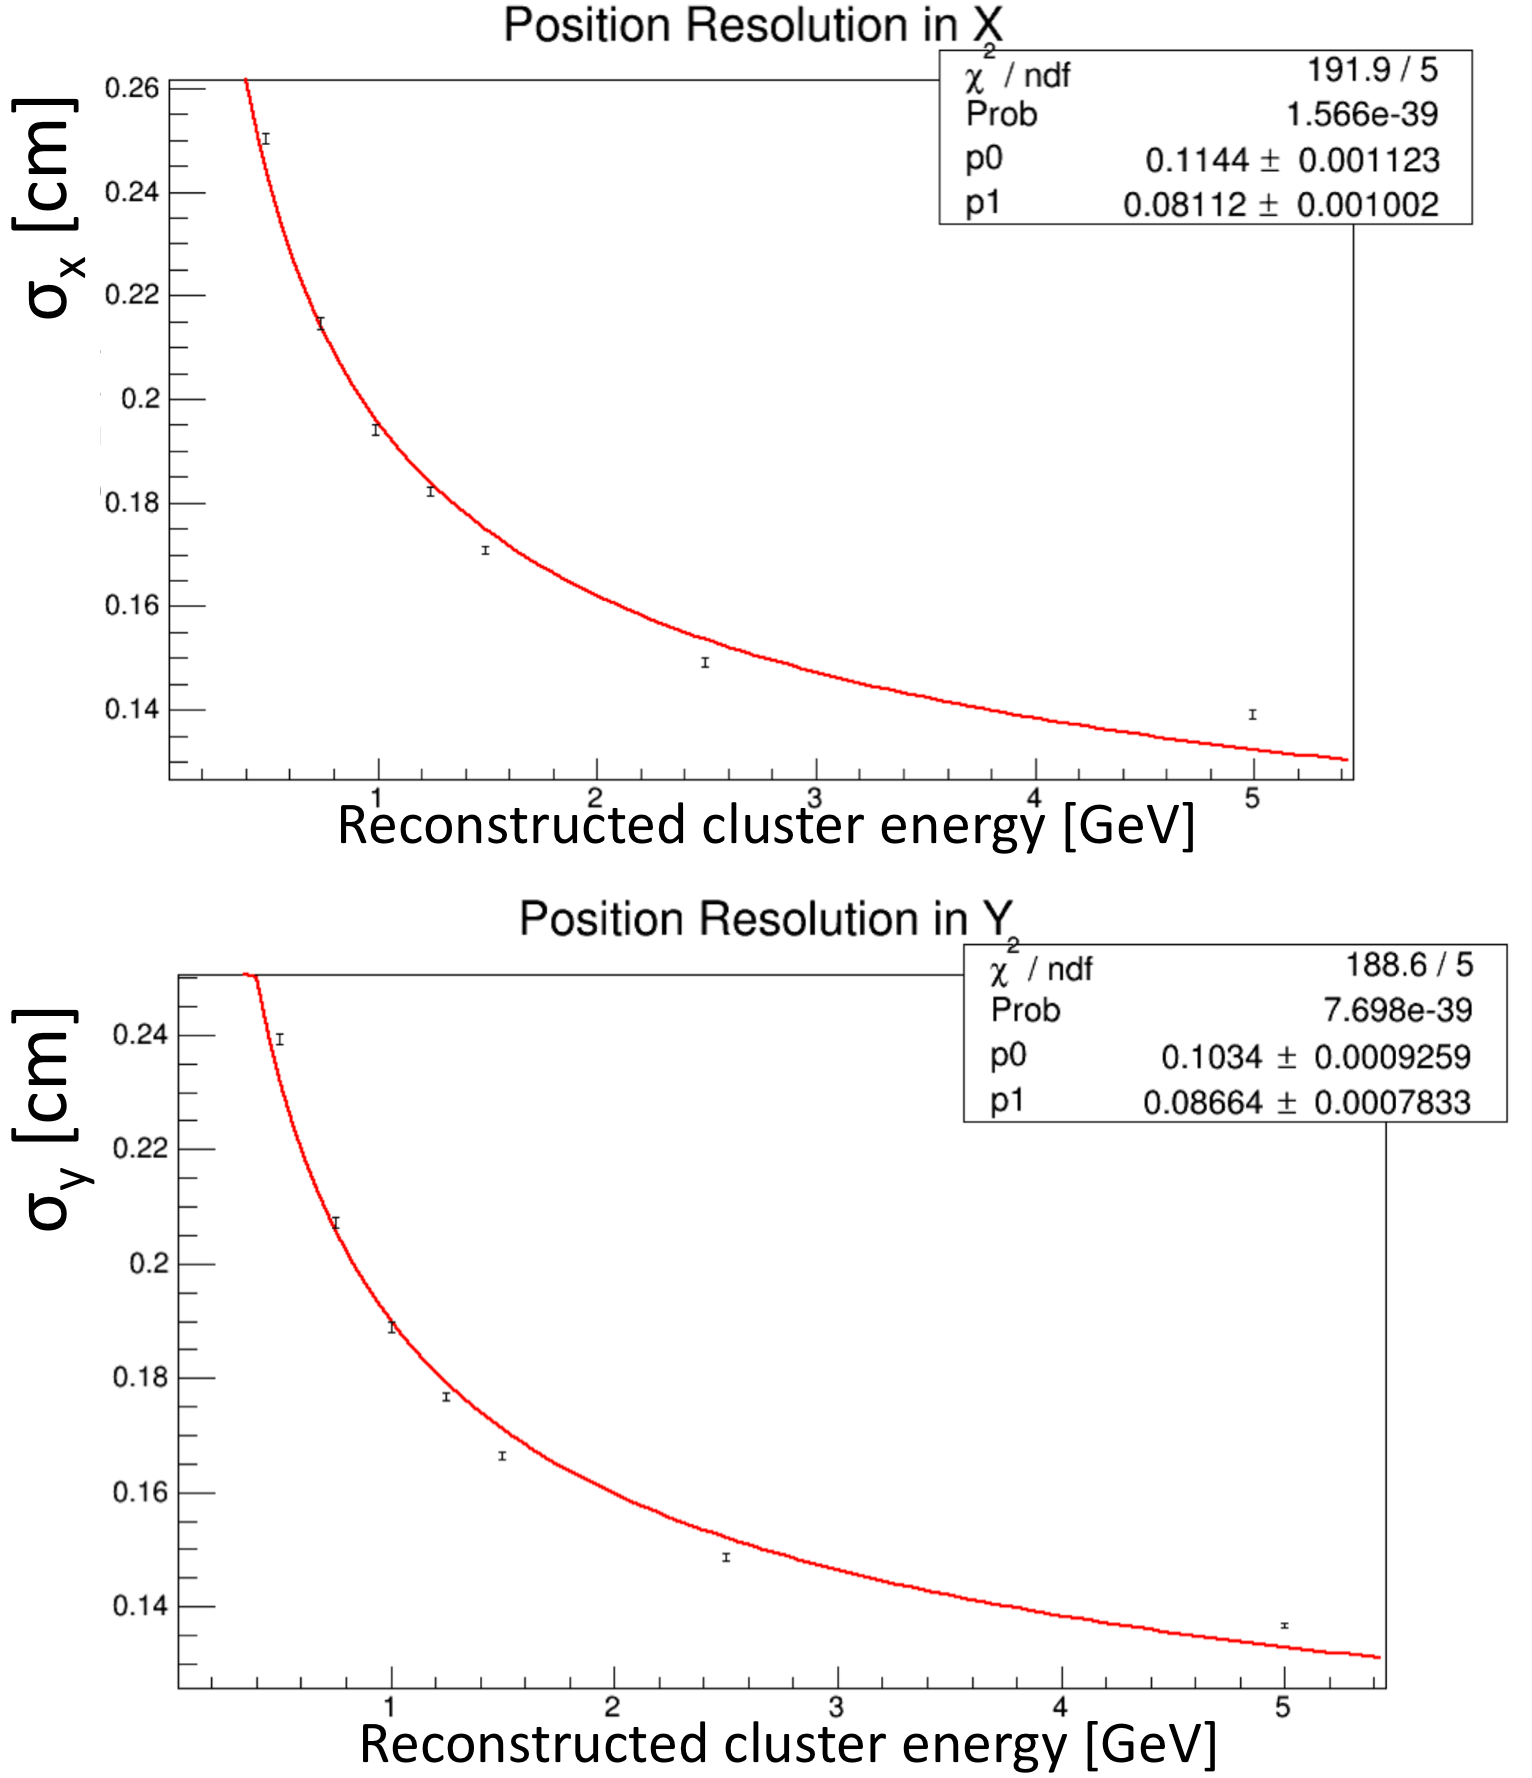
\includegraphics[width=0.9\textwidth]{pics/performance/emPosnResn.png}
  \caption[Energy-dependent position resolution for electrons.]{The energy-dependence of the position resolution for electrons.}
  \label{Figure:emPosnResn}
\end{figure}

The position resolution is parameterized in terms energy following Equation~\eqref{eq:posnRes}.
 
\begin{eqnarray*}
\label{eq:posnRes}
\sigma_x & = & \dfrac{p0_x}{\sqrt{E}}+p1_x\\
\sigma_y & = & \dfrac{p0_y}{\sqrt{E}}+p1_y
\end{eqnarray*}

The parameters $p0$ and $p1$ are found by fitting the residuals for the energies. The position resolution is better than 2~mm for 1~GeV electrons. As the ECal face is located at  approximately 1.4~m from the target, the ECal provides valuable position information when matched with a track. The position resolution for all particle types in the ECal is summarized in Table~\ref{tab:PosnResTable}. 

\begin{table}[H]
\caption{Position resolution.}
\label{tab:PosnResTable}
\centering
\begin{tabular}{|c|c|c|}
\toprule
%\multicolumn{2}{c}{Name} \\
%\cmidrule(r){1-2}
Particle & $\sigma_x$ [mm] & $\sigma_y$ [mm] \\
\midrule
electron & $0.1144/\sqrt{E_{rec}}+0.08112$ & $0.1034/\sqrt{E_{rec}}+0.08664$ \\
positron & $0.1268/\sqrt{E_{rec}}+0.07711$ & $0.1068/\sqrt{E_{rec}}+0.08423$ \\
photon & $0.1255/\sqrt{E_{rec}}+0.08877$ & $0.1005/\sqrt{E_{rec}}+0.08867$ \\
\bottomrule
\end{tabular}
\end{table}

\subsection{Calibration using cosmic ray energy}
The large area APDs enabled the ECal to have the sensitivity to detect signals from cosmic muons traversing the ECal crystals perpendicularly. This signal was used for the initial calibration of the modules. The experimental setup was modeled using Monte Carlo simulations so that the energy deposited in the crystals from cosmic ray muons and rates could be studied. By measuring the average path length of cosmic ray muons in each crystal, the energy deposited in each crystal of the ECal was calculated using the known energy deposition from 2~GeV muons \cite{Agashe:2014kda}. 

The experimental setup for the cosmic calibrations used two scintillators placed below the ECal to trigger readout of all of the crystals. A schematic for the setup of the cosmic calibration is shown in Fig.~\ref{Figure:cosmicScheme}.

%include some discussion of the improvement achieved after removing the splitters

\begin{figure}[H]
  \centering
      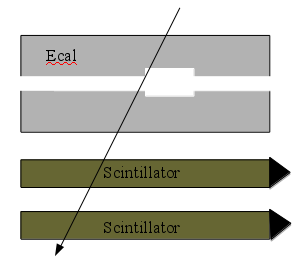
\includegraphics[width=0.5\textwidth]{pics/performance/cosmicschematic.png}
  \caption[Setup for ECal cosmic ray calibration]{Experimental setup for the cosmic ray calibration. As a cosmic ray passe vertically through both scintillators, event readout is triggered.}
  \label{Figure:cosmicScheme}
\end{figure}

Each scintillator measures 75~cm long, 22~cm wide and 5~cm thick covering a slightly larger perpendicular area than the ECal crystals. The two scintillators are less than half a meter apart with the closest scintillator less than half a meter beneath the ECal. The energy deposited in each crystal in a layer is sensitive to the path length of the track as it passed through the crystal. From simulation, the average energy deposited in a crystal by a cosmic ray passing vertically though the ECal is shown in Fig.~\ref{Figure:cosmicEdep}.

\begin{figure}[H]
  \centering
      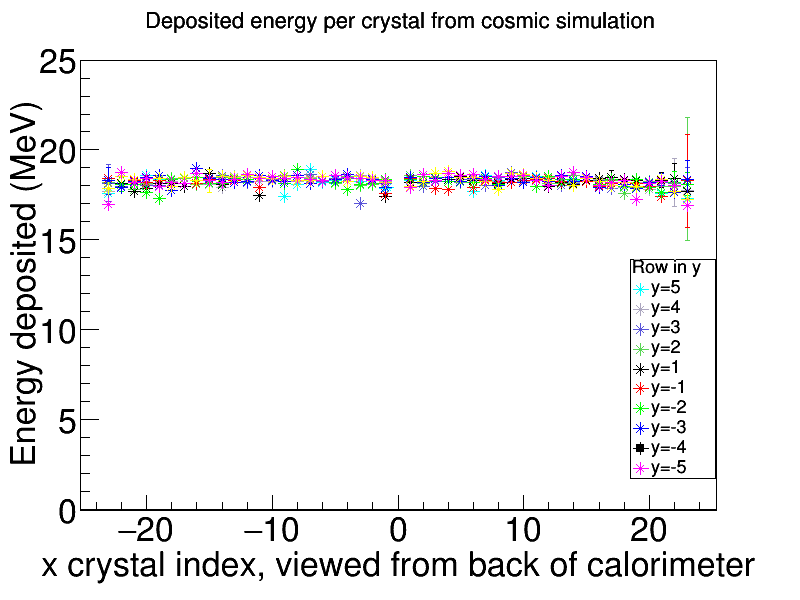
\includegraphics[width=0.8\textwidth]{pics/performance/cosmicEdep.png}
  \caption[Simulation of energy deposited per ECal module from cosmic rays]{The simulated cosmic ray muon energy deposition per crystal of the ECal. The mean energy was 18.3~MeV.}
  \label{Figure:cosmicEdep}
\end{figure}

In Fig.~\ref{Figure:cosmicEdep}, only tracks passing through one crystal in a row were included. Additinally, the cosmic ray muon track had to pass through an adjacent crystal in the row above and below a crystal. For crystals near edges, the geometrical requirement was adjusted to include the two crystals immediately above (or below for cases where the edge is above the crystal) the crystal being readout. The average energy deposited per crystal is approximately 18.3~MeV from the PDG. 

In data, the raw FADC waveform for each crystal is readout, and the event is kept for further study after applying strict coincidence cuts between the two scintillators. The trigger rate for data is about 7~Hz. 30$\%$ of events passed the coincidence cut between the scintillators. For a track passing vertically through all ten layers, we can see the signal in each crystal as shown in Fig.~\ref{Figure:cosmicSig}.

\begin{figure}[H]
  \centering
      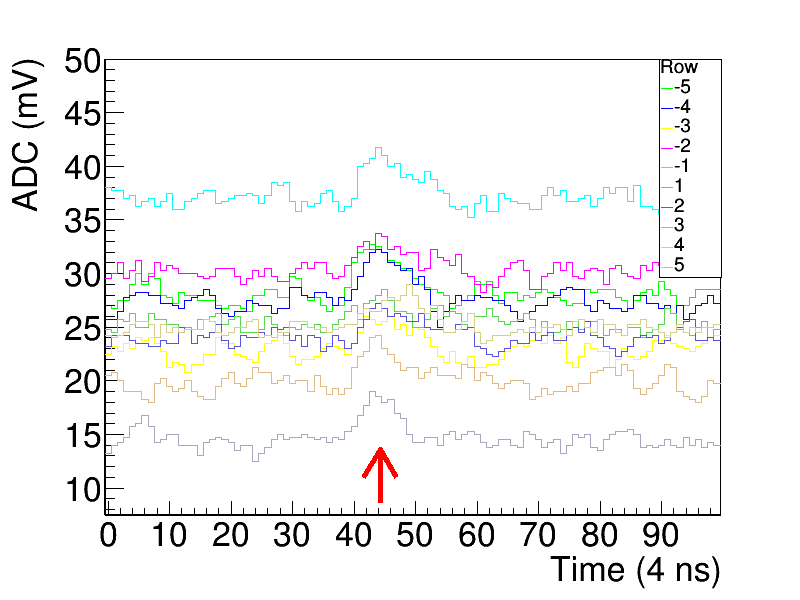
\includegraphics[width=0.7\textwidth]{pics/performance/cosmicSignal.png}
  \caption[Real cosmic ray signal in raw FADC waveform passing vertically through ECal]{Cosmic ray signal passing vertically through all ten layers of crystals in the ECal. Each crystal's signal is separated vertically in this plot by its pedestal. The arrow indicates the approximate place in time that the cosmic signal passed through the detector.}
  \label{Figure:cosmicSig}
\end{figure}

As seen in Fig.~\ref{Figure:cosmicSig}, each FADC channel has a unique pedestal value. The pedestal for each event was calculated as an average of the first twenty bins of the time window. By searching for a threshold crossing in the time window where cosmic events occurred, the signal was then fully integrated and the pedestal was subtracted. The raw waveform thresholds were 2.5~mV in 2015 and increased to 3.5~mV in 2016 to accommodate the larger signals after the removal of the splitters. Geometric cuts are then applied to the data in offline analysis. Crystals having peaks over a certain threshold must have at least an adjacent crystals located above and below with threshold crossing, but the crystals to the left and right must not cross threshold. These cuts ensure that that the track passed as vertically as possible through the ECal (reducing the variations in path length across each crystal). The integrated signals over many events in each crystal were fit. An individual crystal fit is shown in Fig.~\ref{Figure:cosmicFit}.

\begin{figure}[H]
  \centering
      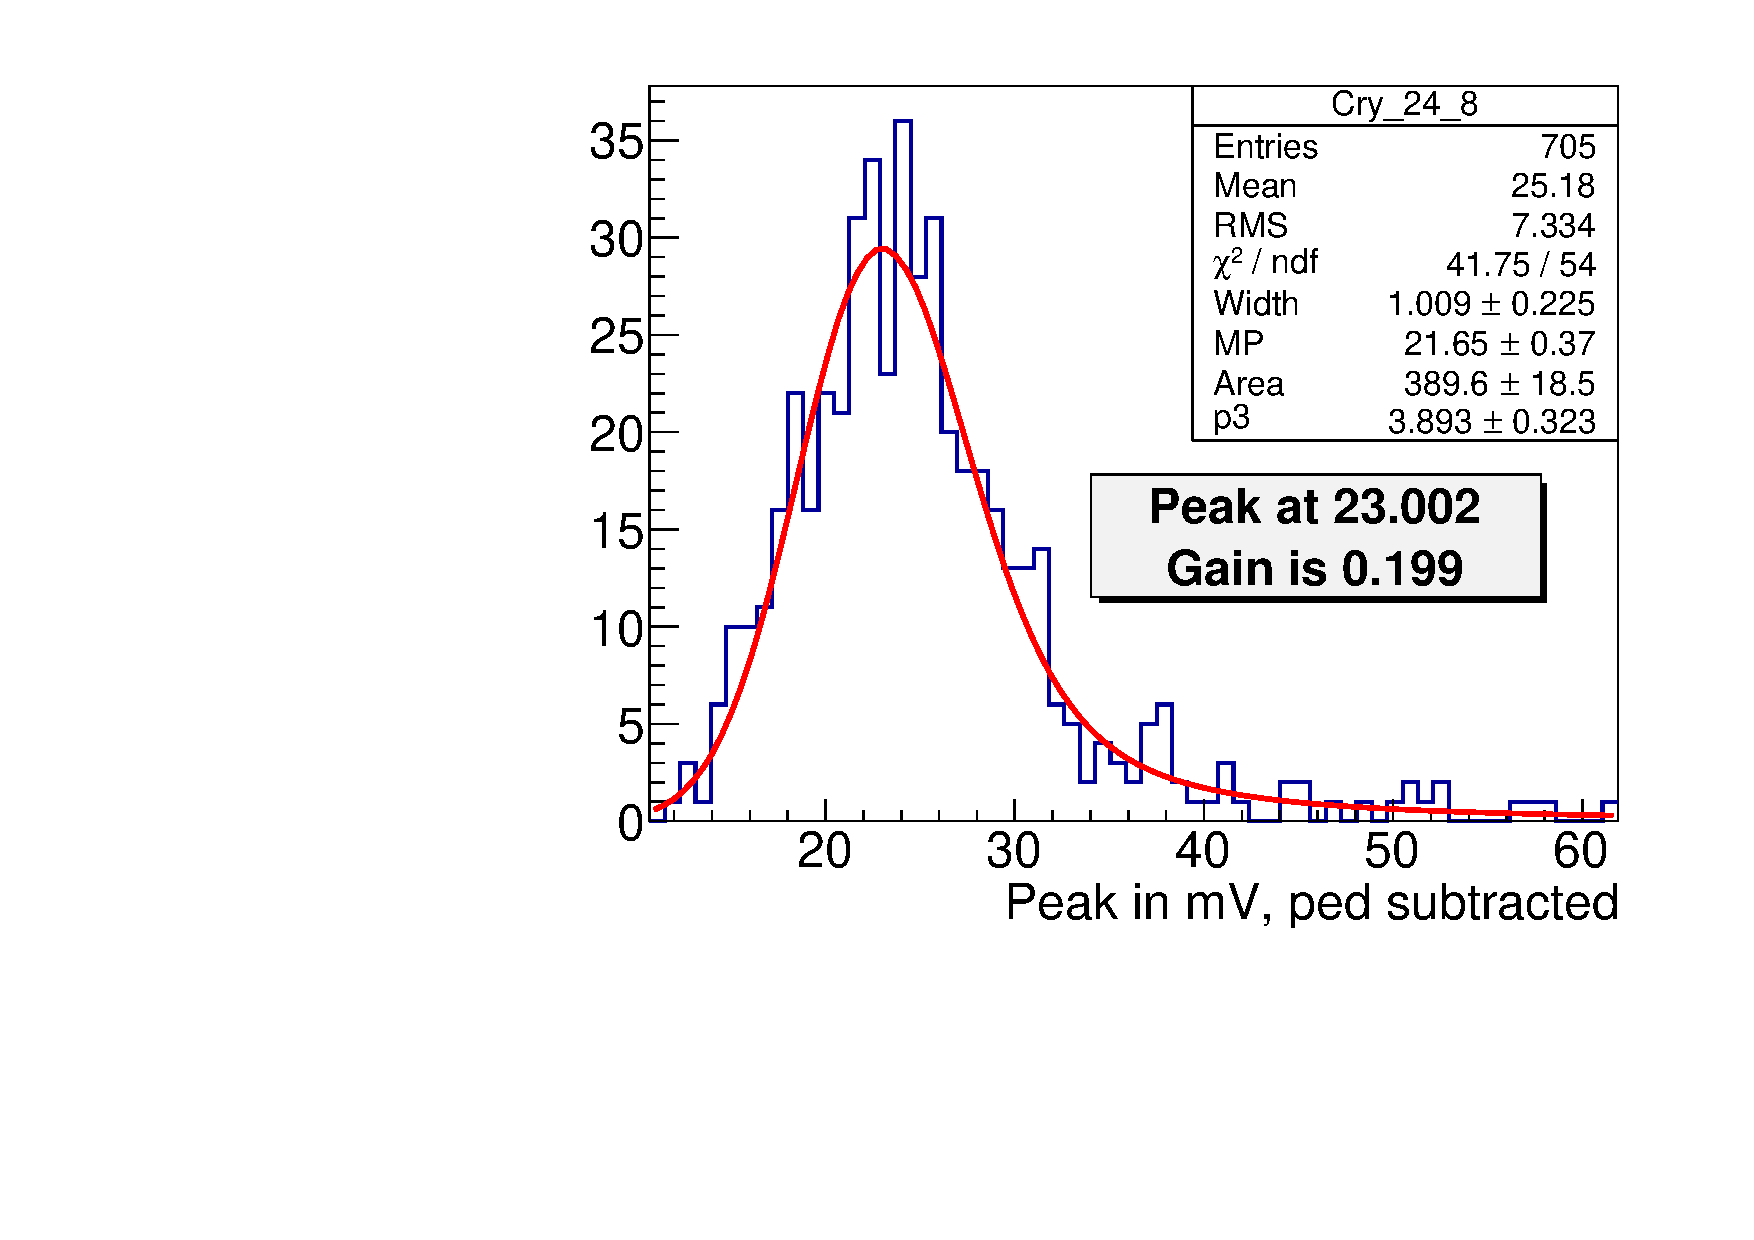
\includegraphics[width=0.8\textwidth]{pics/performance/cosmicFitExample2015.pdf}
  \caption[Integrated cosmic signal in ECal fitted for calibration]{Each cosmic signal was integrated and then fit using a Landau-Gaussian convolution function. The peak was calculated numerically from this fit.}
  \label{Figure:cosmicFit}
\end{figure}

The fit shown in Fig.~\ref{Figure:cosmicFit} utilized a Landau-Gaussian convolution as the Landau part corresponds to the crystal's response to a particle's energy deposition as ionization energy loss, and the Gaussian part accounts for the statistical nature of the electronics shaping and readout. The peak of the fit is calculated numerically, and the initial conversion from units of FADC to energy (MeV) is obtained (called the Gain factor). The unit conversion from units mV to FADC is 1~V to 4096~FADC. The 4096~FADC counts can be set to 1~V or 2~V, but for 2015 and 2016 running, the setting was 1~V. This arises from the 12~bit conversion which yields 4096~FADC. The gain factor is calculated using the measured peak positioin in units of FADC and the known energy deposited from simulation in units of MeV as shown in Eqn.~\eqref{eq:gain}.

\begin{equation}
	\label{eq:gain}
	Gain = \dfrac{[MeV]}{[FADC]} 
\end{equation}

After approximately 60~hours of cosmic data, the full ECal could be calibrated using cosmics, and the resultant gains for all channels in the Engineering Run is shown shown in Fig.~\ref{Figure:cosmicG} and Fig.~\ref{Figure:cosmicGhisto}.

\begin{figure}[H]
  \centering
      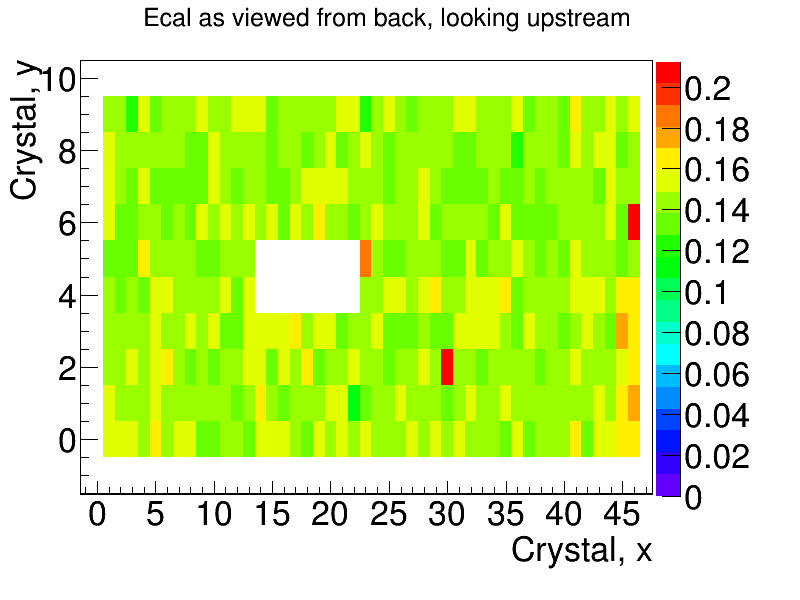
\includegraphics[width=0.7\textwidth]{pics/performance/cosmicGains2015.png}
  \caption[Resulting 2015 gain calibration in the ECal using cosmic ray muons shown by ECal module position]{Resulting gain calibration using cosmics for the Engineering Run.}
  \label{Figure:cosmicG}
\end{figure}


\begin{figure}[H]
  \centering
      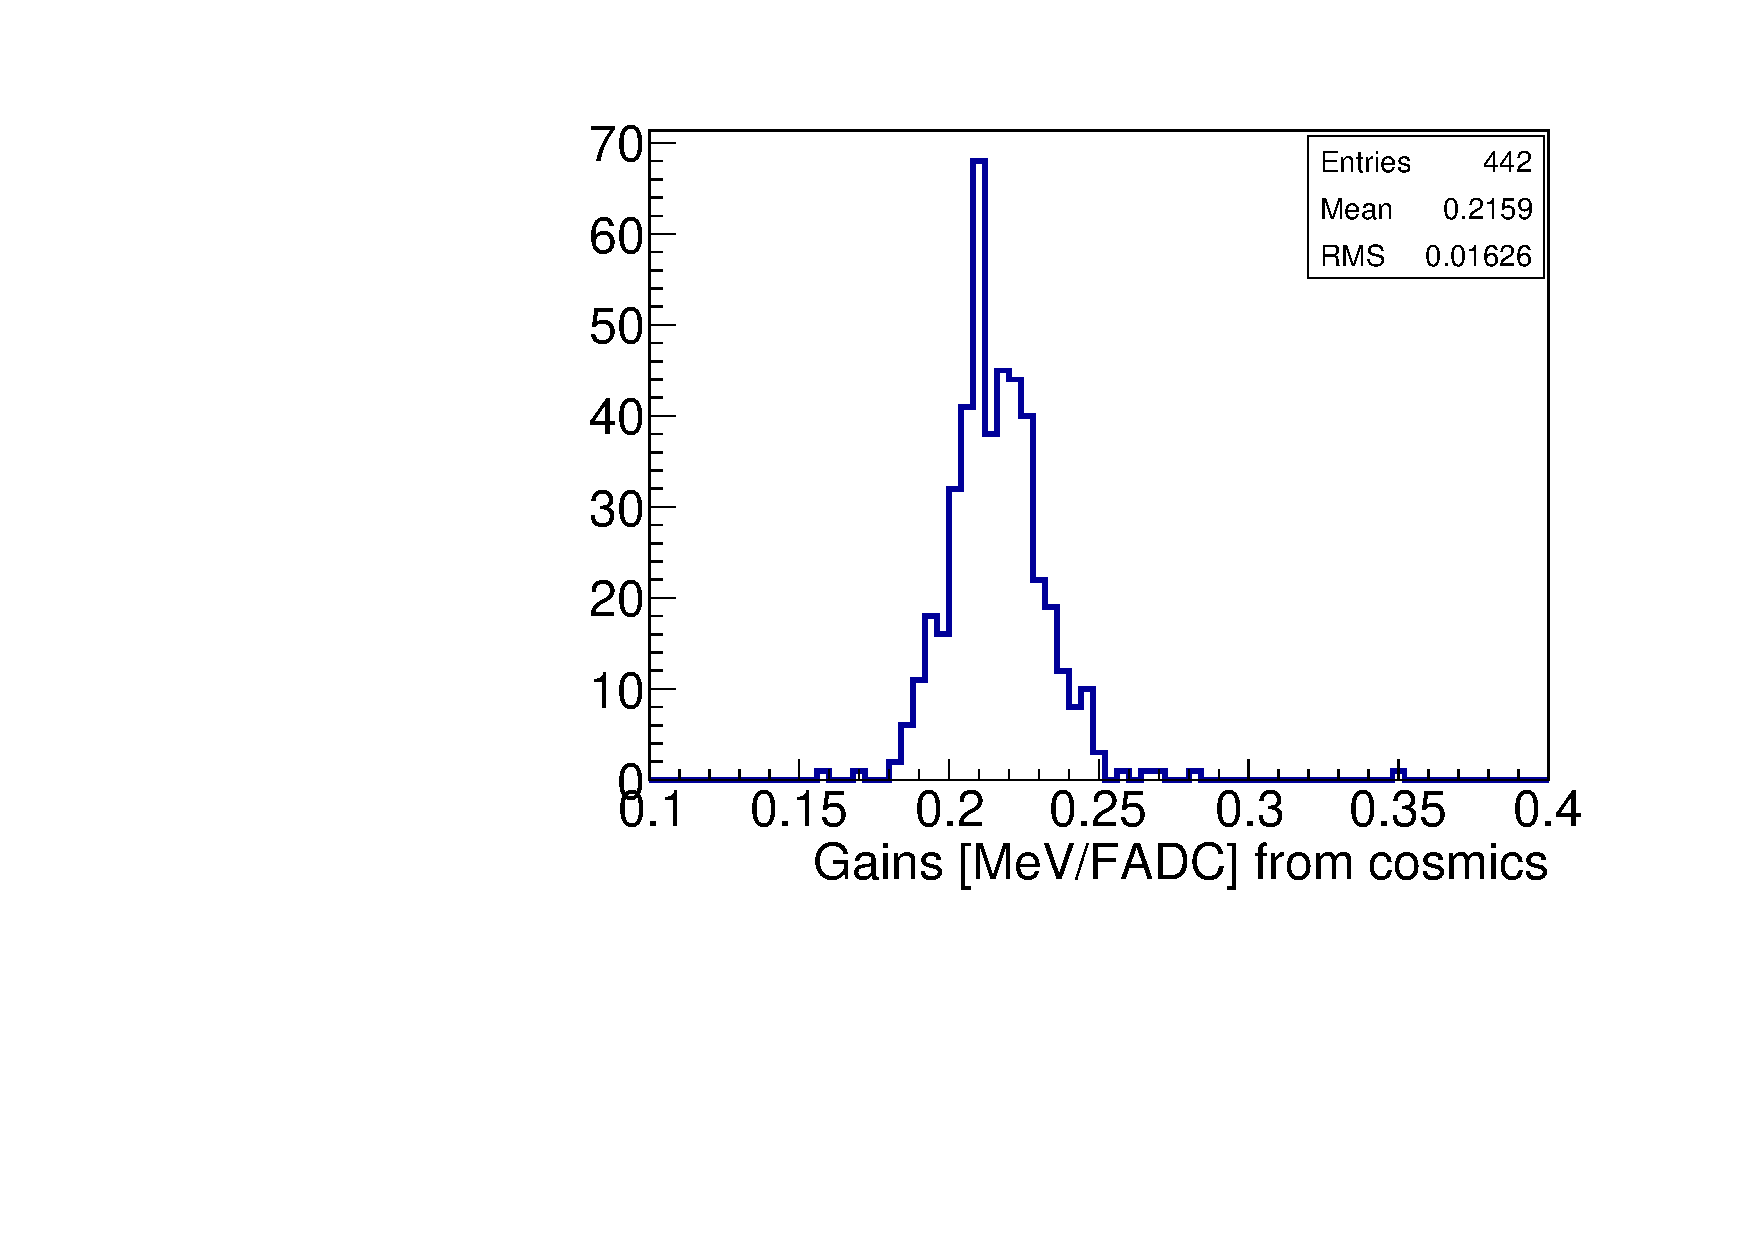
\includegraphics[width=0.7\textwidth]{pics/performance/cosmicGainsMay15.pdf}
  \caption[Distribution of the resulting 2015 gains in the ECal using cosmic ray muons]{Resulting gain calibration using cosmics for the Engineering Run.}
  \label{Figure:cosmicGhisto}
\end{figure}

With the splitters installed in the ECal readout chain, the average gain value was around 0.2~MeV/FADC for the Engineering Run. After the removal of the splitters in January 2016, prior to the Physics Run, the average gains were found to be around 0.13~MeV/FADC.


\subsection{Ecal signal pulse fitting} \label{pulsefitting}
All data was taken using the FADC250 modules which sample at 250~MHz, or every 4~ns. While the firmware has various modes capable of recording data, size was not an issue and Mode 1 was used for all 2015 and 2016 running. Mode 1 is advantageous because the full measured waveform for a module hit is preserved and all methods for extracting the energy and time information from a hit can be done in offline analysis. The trigger decision to readout a module is based off a leading edge threshold which was set to 12~FADC units in 2015. 

The full readout response for each module was carefully studied in order to understand the time response and shaping effects of the preamplifier on the Ecal modules \cite{Charles}. It was found that the raw waveform response was best described by the sum of the pedestal $P$ and a $3-pole$ function for the pulse with width $\tau$ and occurring at time $t_0$ as shown in Eq.~\eqref{eq:thrpole} ~\cite{Charles}.

\begin{equation}
	\label{eq:thrpole}
	P + \dfrac{A}{2\tau^3}(t-t_0)^2e^{-(t-t_0)/\tau} 
\end{equation}

The pulse integral value is parameter $A$. When $t<t_0$, the pulse amplitude is zero. The best resolutions were found by fixing the width parameter for each module as an average of width module as measured over several pulses. An example fit is shown in Fig.~\ref{Figure:mode1fit}.

\begin{figure}[H]
  \centering
      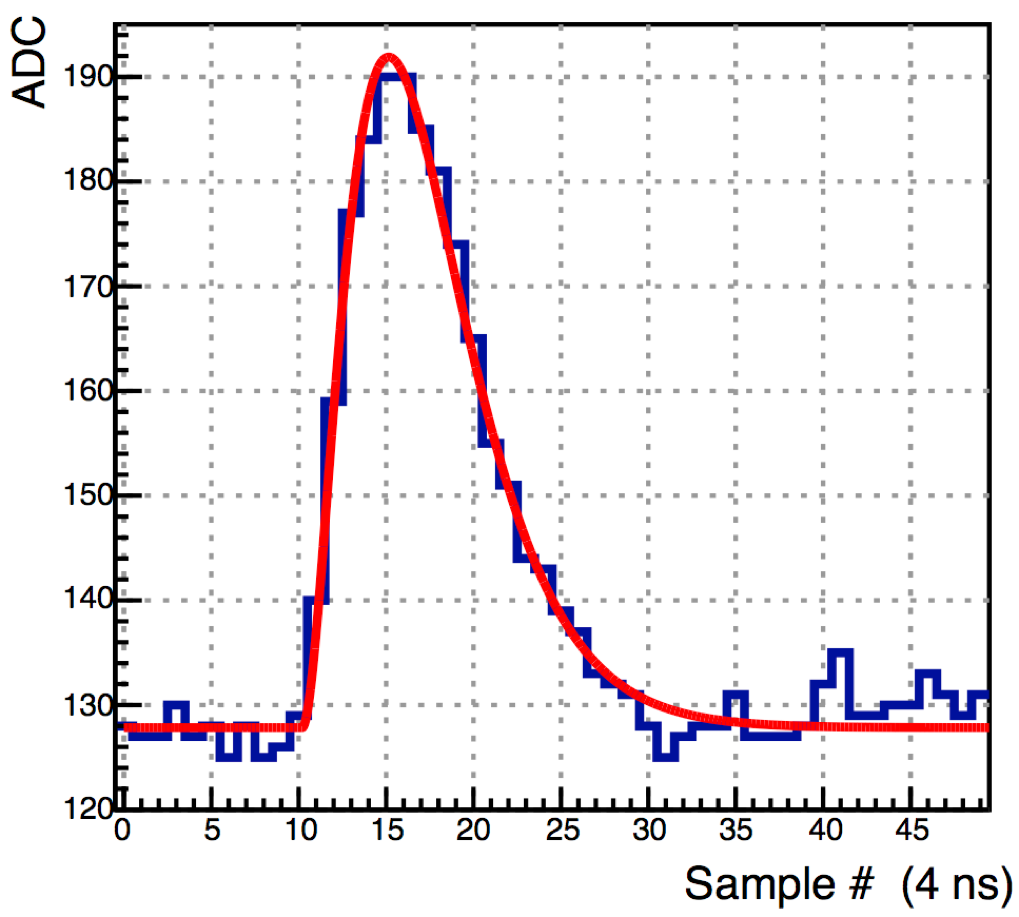
\includegraphics[width=0.5\textwidth]{pics/performance/mode1fit.png}
  \caption[Pulse-fitting to Mode-1 Ecal data]{Example fit to a real Ecal module pulse.}
  \label{Figure:mode1fit}
\end{figure}

The pedestal is calculated event-by-event initialized by a running average over the previous fits for the pulse. The fit range was set to 20~ns before threshold crossing and 60~ns after in order to eliminate pulls from pile-up signals in the same event ~\cite{Baltzell}. The pulse-fitting of the ware waveform demonstrated the best time resolution and energy resolution when compared to the other hardware integral methods that could have been implemented~\cite{Baltzell}.


\subsection{Calibration using elastically-scattered electrons}
The calibration using cosmic ray muons was sufficient for initial data-taking with the electron beam, but the overall energy calibration of the ECal is optimal at higher energies. The ECal detects electrons from elastic scattering at the target that peak, after correction for shower leakage effects, at the beam energy. As the target is off centerline beam right, there are geometric effects that prevent elastically-scattered beam energy electrons from full coverage of the ECal.~\cite{CalibNote} From simulation, the first column of crystals on beam right, and the five columns of crystals on beam left cannot be calibrated using elastically-scattered electrons. \\
\indent To calibrate the ECal using elastically-scattered electrons, we selected events where the seed hit crystal carried at least 60$\%$ of the overall cluster energy. The seed hit was also required to have carried greater than 450~MeV in the 2015 data (1.1~GeV for the 2016 dataset), to have triggered a Singles-1  event readout from the DAQ, and to have occurred in the optimal trigger timing window. The cluster energy was associated with the seed hit module for the calibration. The calibration uses an iterative procedure, by which the reconstructed peak energy is matched to that found by simulation (prior to energy corrections). For each peak, an iteration coefficient is found that reflects the ratio of the peak position measured in Monte Carlo to the peak position found for a particular iteration in the data. This ratio can be seen in Equation~\eqref{eq:feeiter}.

\begin{equation}
	\label{eq:feeiter}
	C_i = \dfrac{MC_{peak}}{data_{peak}}
\end{equation}

After each iteration, this ratio $C_i$ is applied to the to the original gain coefficient as well as any coefficient found from previous iteration. The data is re-processed applying these changes to the gains and clustering is re-run. This procedure continues until the correction coefficients found in a particular iteration are all less than 1$\%$. Crystals on the edge of acceptance with poorly resolved peaks were given an iteration coefficient of 1. After completion of the calibration (approximately 2-3 iterations)~\cite{CalibNote}, the shower loss correction functions were applied to the reconstructed cluster energies. The final peak position for elastically-scattered electron clusters in the fiducial region of the ECal is shown in Figure

\begin{figure}[H]
  \centering
      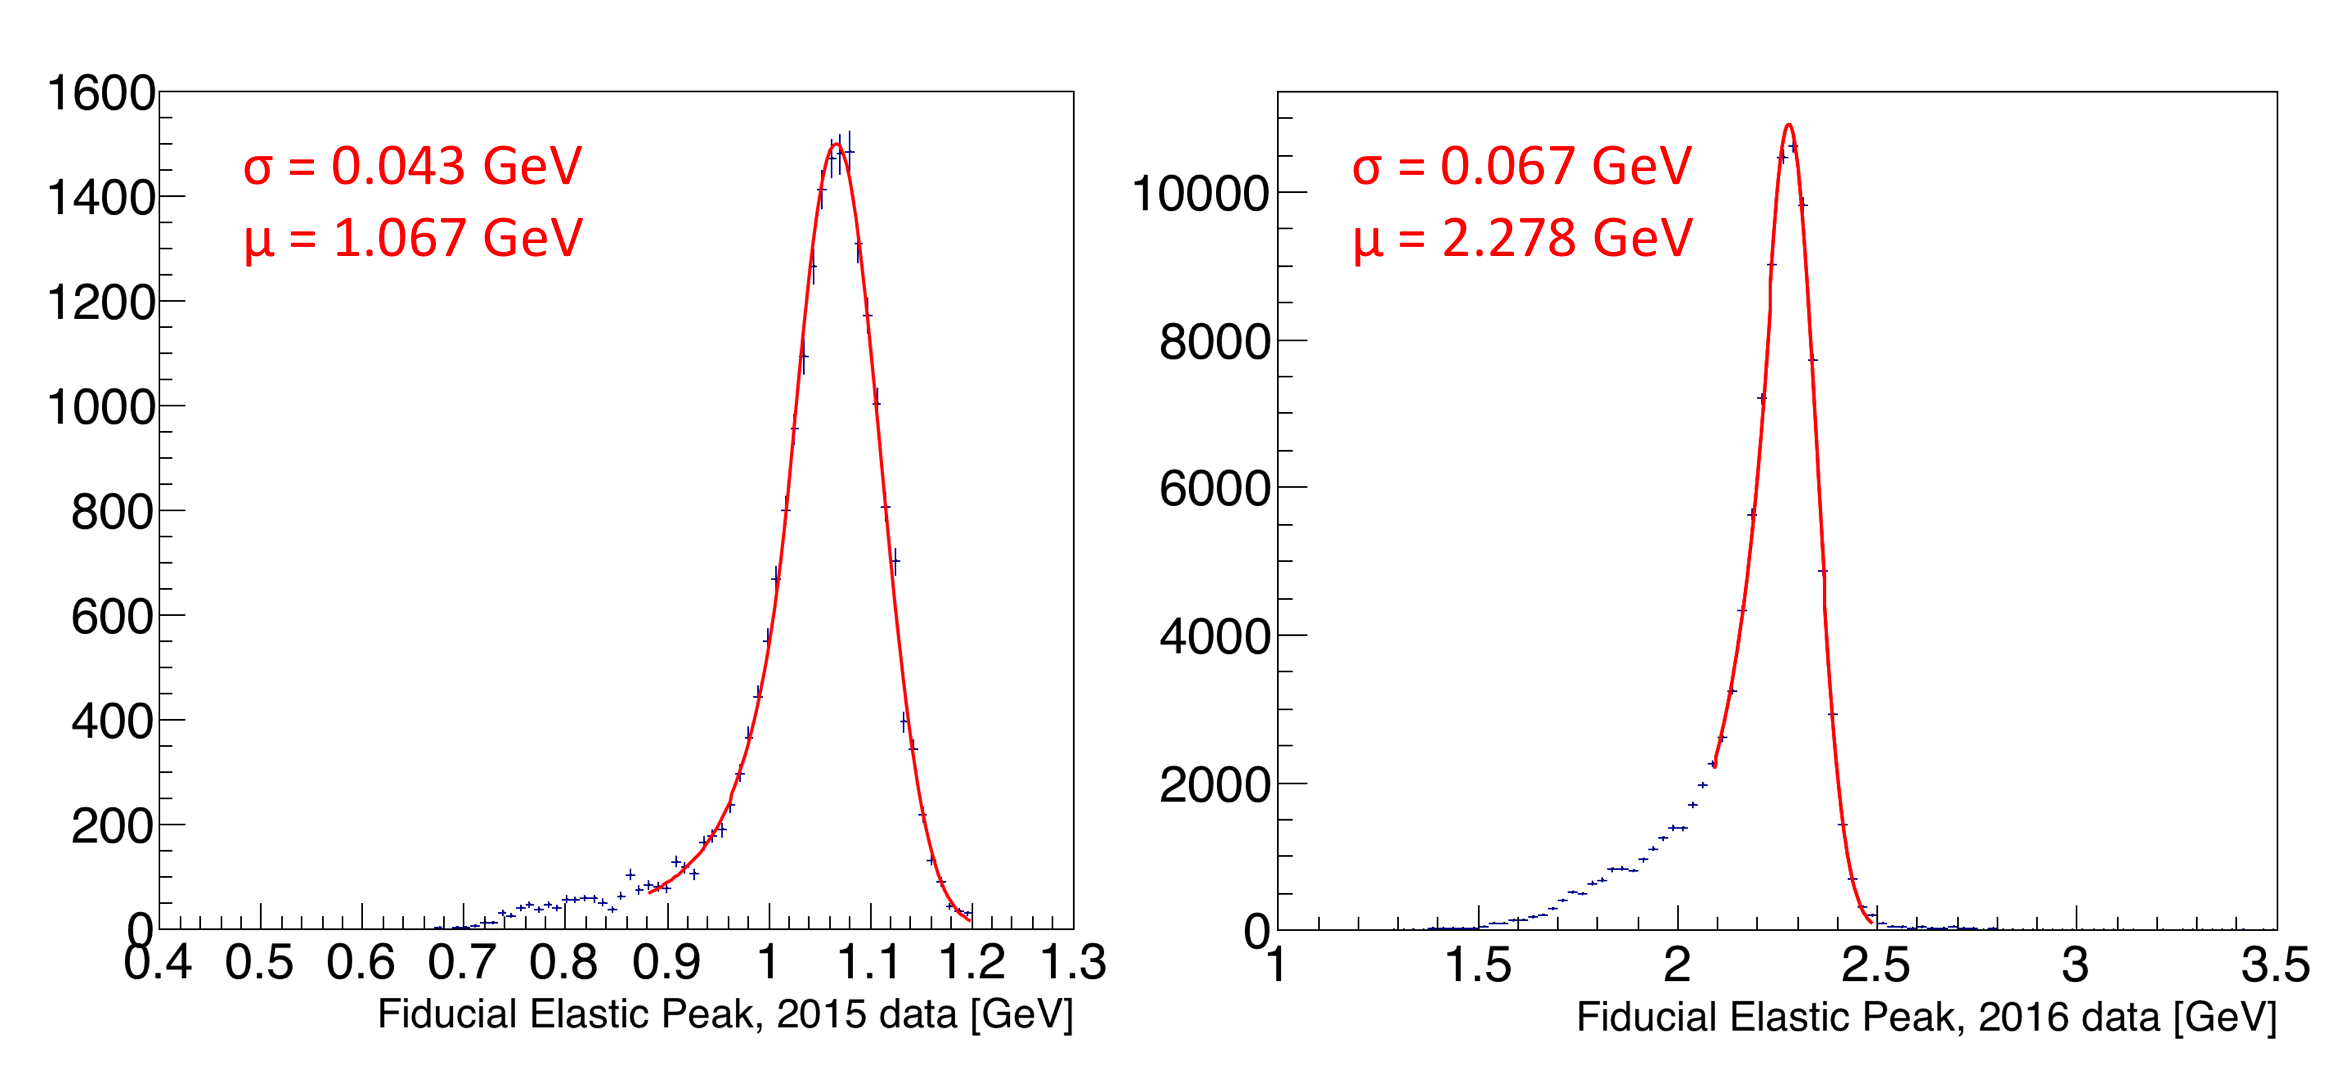
\includegraphics[width=0.9\textwidth]{pics/performance/feePeakFid.png}
  \caption[Reconstructed elastic peak in the ECal for the Engineering and Physics Runs]{Shown are the resultant fiducial peaks for the Engineering and Physics Runs on the left and right, respectively. The peaks are fit with a Crystal Ball function and the peak position and widths are indicated. }
  \label{Figure:FeeFidPeak}
\end{figure}

The energy resolution improves with the beam energy. The cluster energy spectrum is fit with a Crystal Ball function which contains a Gaussian component and a power law low energy tail. The ECal has an energy resolution of approximately 4$\%$ in the fiducial region at approximately 1~GeV and 2.9$\%$ at 2.3~GeV. \\
\indent The final gains obtained after calibration with elastically-scattered electrons were compared to the gains obtained with cosmics alone in order to check for systematic offsets. While no systematic offsets were found, the comparison between the low and high energy calibrations tells us that the initial energies used for the cosmic calibration are roughly accurate, but it is limited in telling us anything about the linearity of the gain between these two energies.~\cite{CalibNote} If there was found to be any systematic offsets, these should be applied to the gains of the crystals that could not be calibrated using the elastically-scattered electrons due to acceptance, and the effects on the triggered data would need to be quantified. 

%\begin{figure}[H]
 % \centering
    %  \includegraphics[width=0.9\textwidth]{pics/performance/cosmicComp.png}
 % \caption[Gain comparison between cosmic and elastic calibration]{A comparison between the gains from he cosmic and elastic calibration is shown. Any overall systematic shift would need to be applied to crystals outside of the elastic calibration acceptance. }
%  \label{Figure:cosmicComp}
%\end{figure}


\subsection{Wide angle bremsstrahlung for studies of edge effects}
The primary physics trigger looks for two cluster events and recorded a high yield of WAB particles composed of a final state electron and photon. The spectrum of cluster energies in the Engineering Run dataset shows an excess of WAB events occurring where the energy sum of the two particles is approximately equal to the uncorrected beam energy.  \\
\indent Initial studies after the calibration using elastic electrons showed that the energy sum of two particles in WAB events having mid-range energies was lower than the reconstructed elastic energy, indicating that the shower loss corrections in the mid-range beam energy required further investigation. WAB events were used to refine the shower loss corrections for mid-range energy particles. WAB events are identified by have track-matched clusters and no track matching a photon cluster. The reconstructed energy sum of of the two particles must be equivalent the beam energy as shown in Equation~\eqref{eq:wabBeam}.~\cite{CalibNote}

\begin{equation}
	\label{eq:wabBeam}
	E_i = \dfrac{E_{e-}}{f_{e-}(E_{e-})}+\dfrac{E_{\gamma}}{f_{\gamma}(E_{\gamma})}
\end{equation}

In Equations~\eqref{eq:wabBeam} and \eqref{eq:wabBeamChi}, $f$ refers to the shower loss correction described by Equation~\eqref{eq:eclsf}. The underlying assumption is that the relationship between the electron and photon shower loss corrections found in Monte Carlo are preserved according to Equation~\eqref{eq:wabRatio}.

\begin{equation}
	\label{eq:wabRatio}
	 \dfrac{f_{e-, data}(E_{e-})}{f_{\gamma, data}(E_{\gamma})}= \dfrac{f_{e-, MC}(E_{e-})}{f_{\gamma, MC}(E_{\gamma})}
\end{equation}

In maintaining the relationships shown in Equations~\eqref{eq:wabBeam} and \eqref{eq:wabRatio}, a chi-squared minimization yields the optimal adjustments to the shower loss correction functions for mid-range energy particles as shown in Equation~\eqref{eq:wabBeamChi}.

\begin{equation}
	\label{eq:wabBeamChi}
	\chi^2 =\sum_{i} \dfrac{(E_{beam}-E_i)^2}{\sigma_{e-}^2(E_{e-})+\sigma_{\gamma}^2(E_{\gamma})}	
\end{equation}

For each event, the energy sum of the two corrected clusters, $E_i$, is calculated as described by Equation~\eqref{eq:wabBeamChi}.The end result is a small correction to the shower loss correction functions that ranges across the cluster energies and never exceeds a difference of 2$\%$.~\cite{CalibNote} After incorporating these updated corrections to the shower loss correction functions, the energy resolution can be extracted for all energies and positions in the ECal.  


\subsection{Energy resolution in data}
The elastically-scattered electrons provided the clearest point in extracting the energy resolution of the Ecal at the beam energy. Using WAB particles, electrons and photons, the energy resolution of the Ecal was fully characterized in terms of energy and position relative to the edges.\\
\indent To study the energy resolution in the fiducial region of the Ecal, all electrons were matched to tracks, and the track position extrapolated to the incident face of the Ecal was used to determine the electron's vertical distance relative to the beam gap edge. For elastically-scattered electrons, one track-matched electron is used. For WAB electrons, the photon cluster was required to be at least 10~mm from the Ecal edges as this way, the reconstructed photon energy is reliable. By selecting WAB events where the energy difference between the two particles is less than 100~MeV, the resolution of the energy sum peak was fitted to extract the resolution. The resolution was extracted according to Equation~\eqref{eq:eResExtract}.

\begin{equation}
	\label{eq:eResExtract}
	\sigma_{E_{\gamma}+E_{e-}}^2 = \sigma_{e-}^2(E_{e-})+\sigma_{\gamma}^2(E_{\gamma})
\end{equation}

When both particles are in the fiducial region and are roughly equal in energy, then the energy resolution of the sum could be divided by $\sqrt{2}$ assuming that the energy resolution of both particles is the same. This same procedure was used to study the resolution when the particle energies were more asymmetric in energy in order to obtain the single particle energy resolution at various energies. \\
\indent The experimentally-obtained fiducial energy resolution agrees well with Monte Carlo but generally yields a slightly larger energy resolution across all energies (on the order of about 15$\%$). The energy resolution obtained in data is shown in Figure~\ref{Figure:eResData}.

\begin{figure}[H]
  \centering
      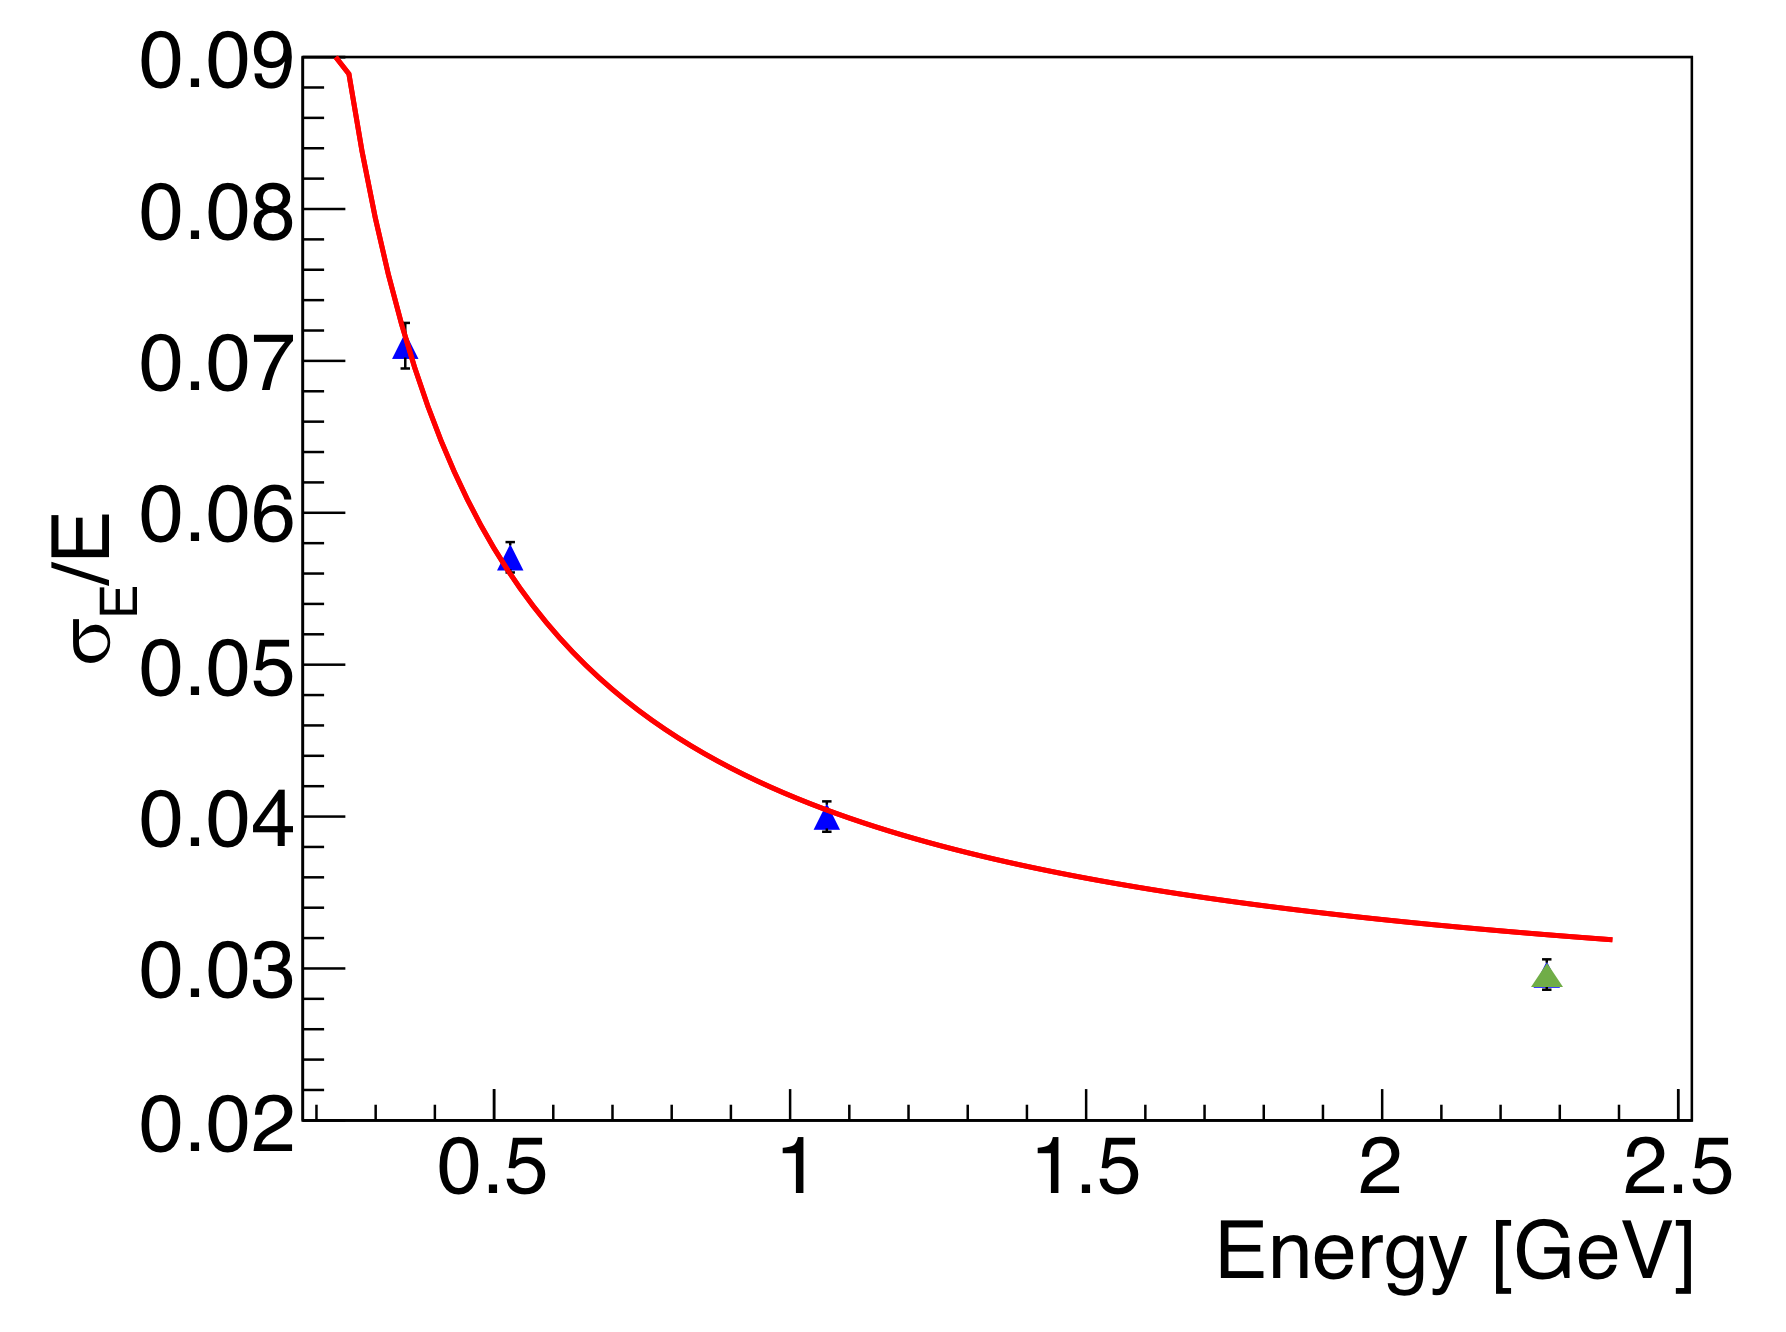
\includegraphics[width=0.9\textwidth]{pics/performance/eResData.png}
  \caption[Energy resolution of the Ecal found in data]{The blue points are derived from the 2015 running for the energy resolution of a single particle. The green point at approximately 2.3~GeV was determined from the elastic calibration of the 2016 data. The fitted energy resolution was determined from the 2015 data only, but it shown here extrapolated to the 2016 energy.}
  \label{Figure:eResData}
\end{figure}

The fit to the energy resolution in data is shown in Equation~\eqref{eq:eResData} and is fit to the blue points representative of the 2015 data in Figure~\ref{Figure:eResData}.

\begin{equation}
	\label{eq:eResData}
	\dfrac{\sigma_E}{E}(\%) = \dfrac{1.62}{E}\bigoplus\dfrac{2.87}{\sqrt{E}}\bigoplus2.5
\end{equation}

The first term in Equation~\eqref{eq:eResData} is generally attributed to the noise from the pre-amplifiers and is roughly consistent to that found in Monte Carlo. The second term is related to the statistical fluctuations of the shower containment and the APD gain. This term is larger than the term found in Monte Carlo but is still roughly consistent. The third term contains both the energy leakage out the back of the Ecal as well as the crystal-to-crystal inter-calibration error. This term is significantly higher than that derived in Monte Carlo, but is much closer to the term as found in data for the CLAS Inner Calorimeter. It's possible that this term is affected by the inability to calibrate several crystals along the outer edges of the calorimeter with elastics. \\
\indent The energy resolution as found in 2016 at 2.3~GeV (shown in green on Figure~\ref{Figure:eResData}) is slightly better than that predicted by the fit to the 2015 points. It is likely that the energy resolution of the Ecal improved overall in 2016 as compared to 2015 because the TDCs were removed, and the signal going into the FADCs was no longer split. 


\subsection{Timing calibration and performance}
The time obtained from the raw fitting of the waveform requires corrections in order to account for various crystal-to-crystal time offsets that can result due to time walk and differences in hardware (such as cable lengths). The overall time offset for each crystal can be corrected using the accelerator RF signal, and the time walk can be removed through study of hits and hit energies in a cluster versus that of the seed hit energy. The corrected individual crystal time is shown in Equation~\eqref{eq:toff}.

\begin{equation}
	\label{eq:toff}
	t = t_0 +\Delta t_{RF} + \Delta t_w (E)
\end{equation}

In Equation~\eqref{eq:toff}, $t_0$ is the time calculated from fit to the raw ADC distribution of a crystal, $\Delta t_{RF}$ is the hit time offset with the accelerator RF signal, and $\Delta t_w(E)$ is the energy-dependent time-walk correction. The accelerator has a an intrinsic frequency of 499 MHz, and the RF signal is sampled every 80 signals into Hall B. The RF signal in the hall is readout by two FADC250 channels. The raw waveform of the RF signal is shown in Figure~\ref{Figure:rfFits}. 

\begin{figure}[H]
  \centering
      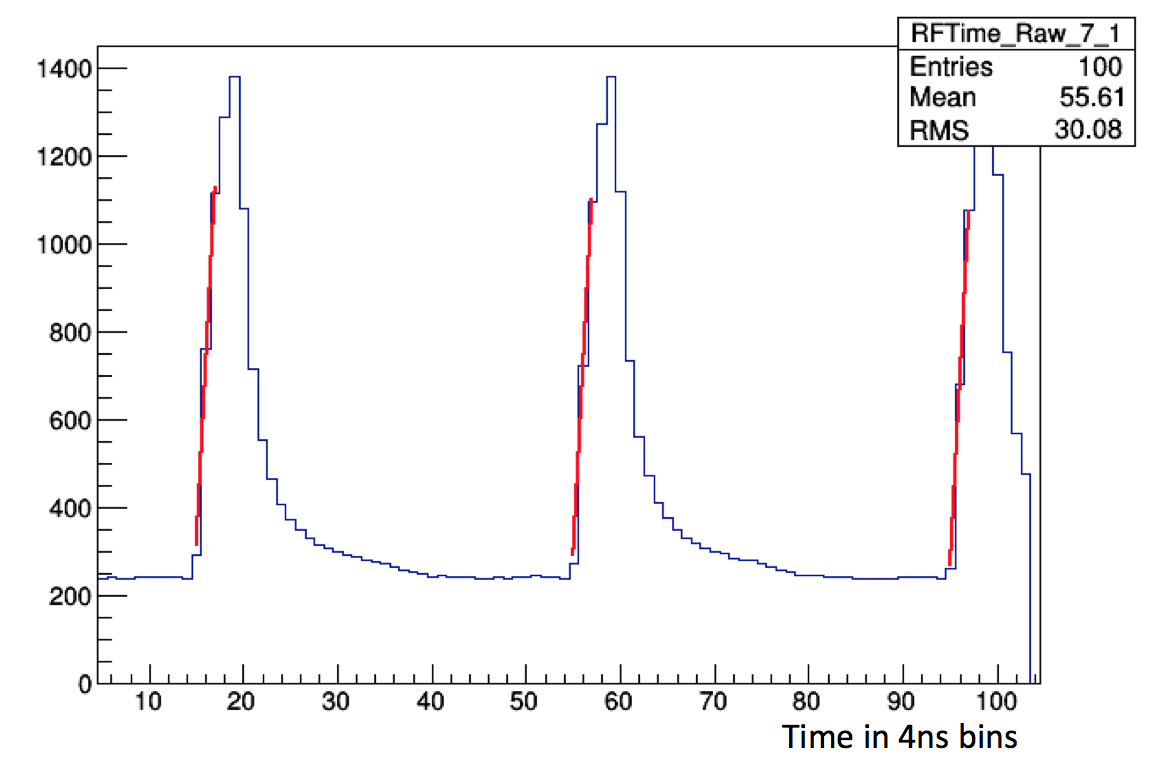
\includegraphics[width=0.7\textwidth]{pics/performance/rfFits.png}
  \caption[Fitted, raw waveform of the RF signal in HPS]{The raw distribution of the RF signal is shown with a straight line fit to the leading edge of the signal.}
  \label{Figure:rfFits}
\end{figure}

The strategy to read off the time from the RF signal was chosen in order to minimize the measured intrinsic resolution of the FADC modules. After identifying the peak bin (4~ns per bin), the pedestal was calculated by averaging the values in 4 bins occurring at 6 to 9 samples prior to the peak. The threshold used in selecting the fitting points was found by calculating the 1/3 height between the averaged pedestal and the peak. The points for the straight line fit were then chosen as the last point below this threshold and the next two points above the threshold. These points were chosen due to the linear uniformity of the pulse away from the
peak bin. The time that was used from this fit was at the half height between the pedestal and the peak. This combination of parameters minimized the width of the time difference distribution between the RF signals in the two FADC channels as shown in Figure~\ref{Figure:intrTres}. 

\begin{figure}[H]
  \centering
      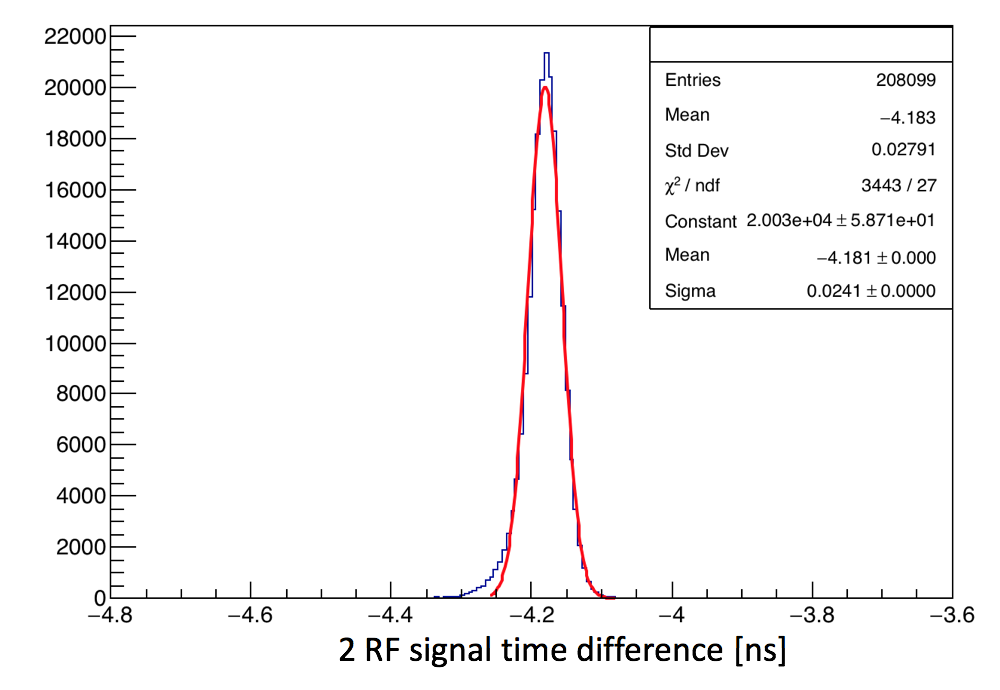
\includegraphics[width=0.7\textwidth]{pics/performance/rfRes.png}
  \caption[FADC intrinsic time resolution]{The intrinsic time resolution of the FADC modules can be obtained by the width of the two RF signal time difference to be approximately 24~ps.}
  \label{Figure:intrTres}
\end{figure}

The internal time resolution of the FADC modules was measured to be approximately 24~ps from the width of the time difference between the two RF signals. The individual crystal module time offsets are measured with respect to the accelerator RF time. For time offsets less than 2~ns, or the time between electron bunches from the accelerator, we calculate the fine time offset per crystal as shown in Equation~\eqref{eq:tfine}.

\begin{equation}
	\label{eq:tfine}
	\Delta t_{fine} = modulo(t_0 - t_{RF} + N\times 2.004, 2.004) - 1.002 \textsf{ ns}
\end{equation}

In Equation~\eqref{eq:tfine}, $t_0$ is the time for the crystal as reported from pulse-fitting, $t_{RF}$ is the reported RF time, and $N$ is an arbitrarily large integer to shift the distribution to all positive values. 2.004~ns pertains to 499~MHz accelerator RF frequency. Before applying Equation~\eqref{eq:tfine}, we observe the beam bunch structure in the time difference between the crystal hits and the RF time in Figure~\ref{Figure:beamBunch}. 

\begin{figure}[H]
  \centering
      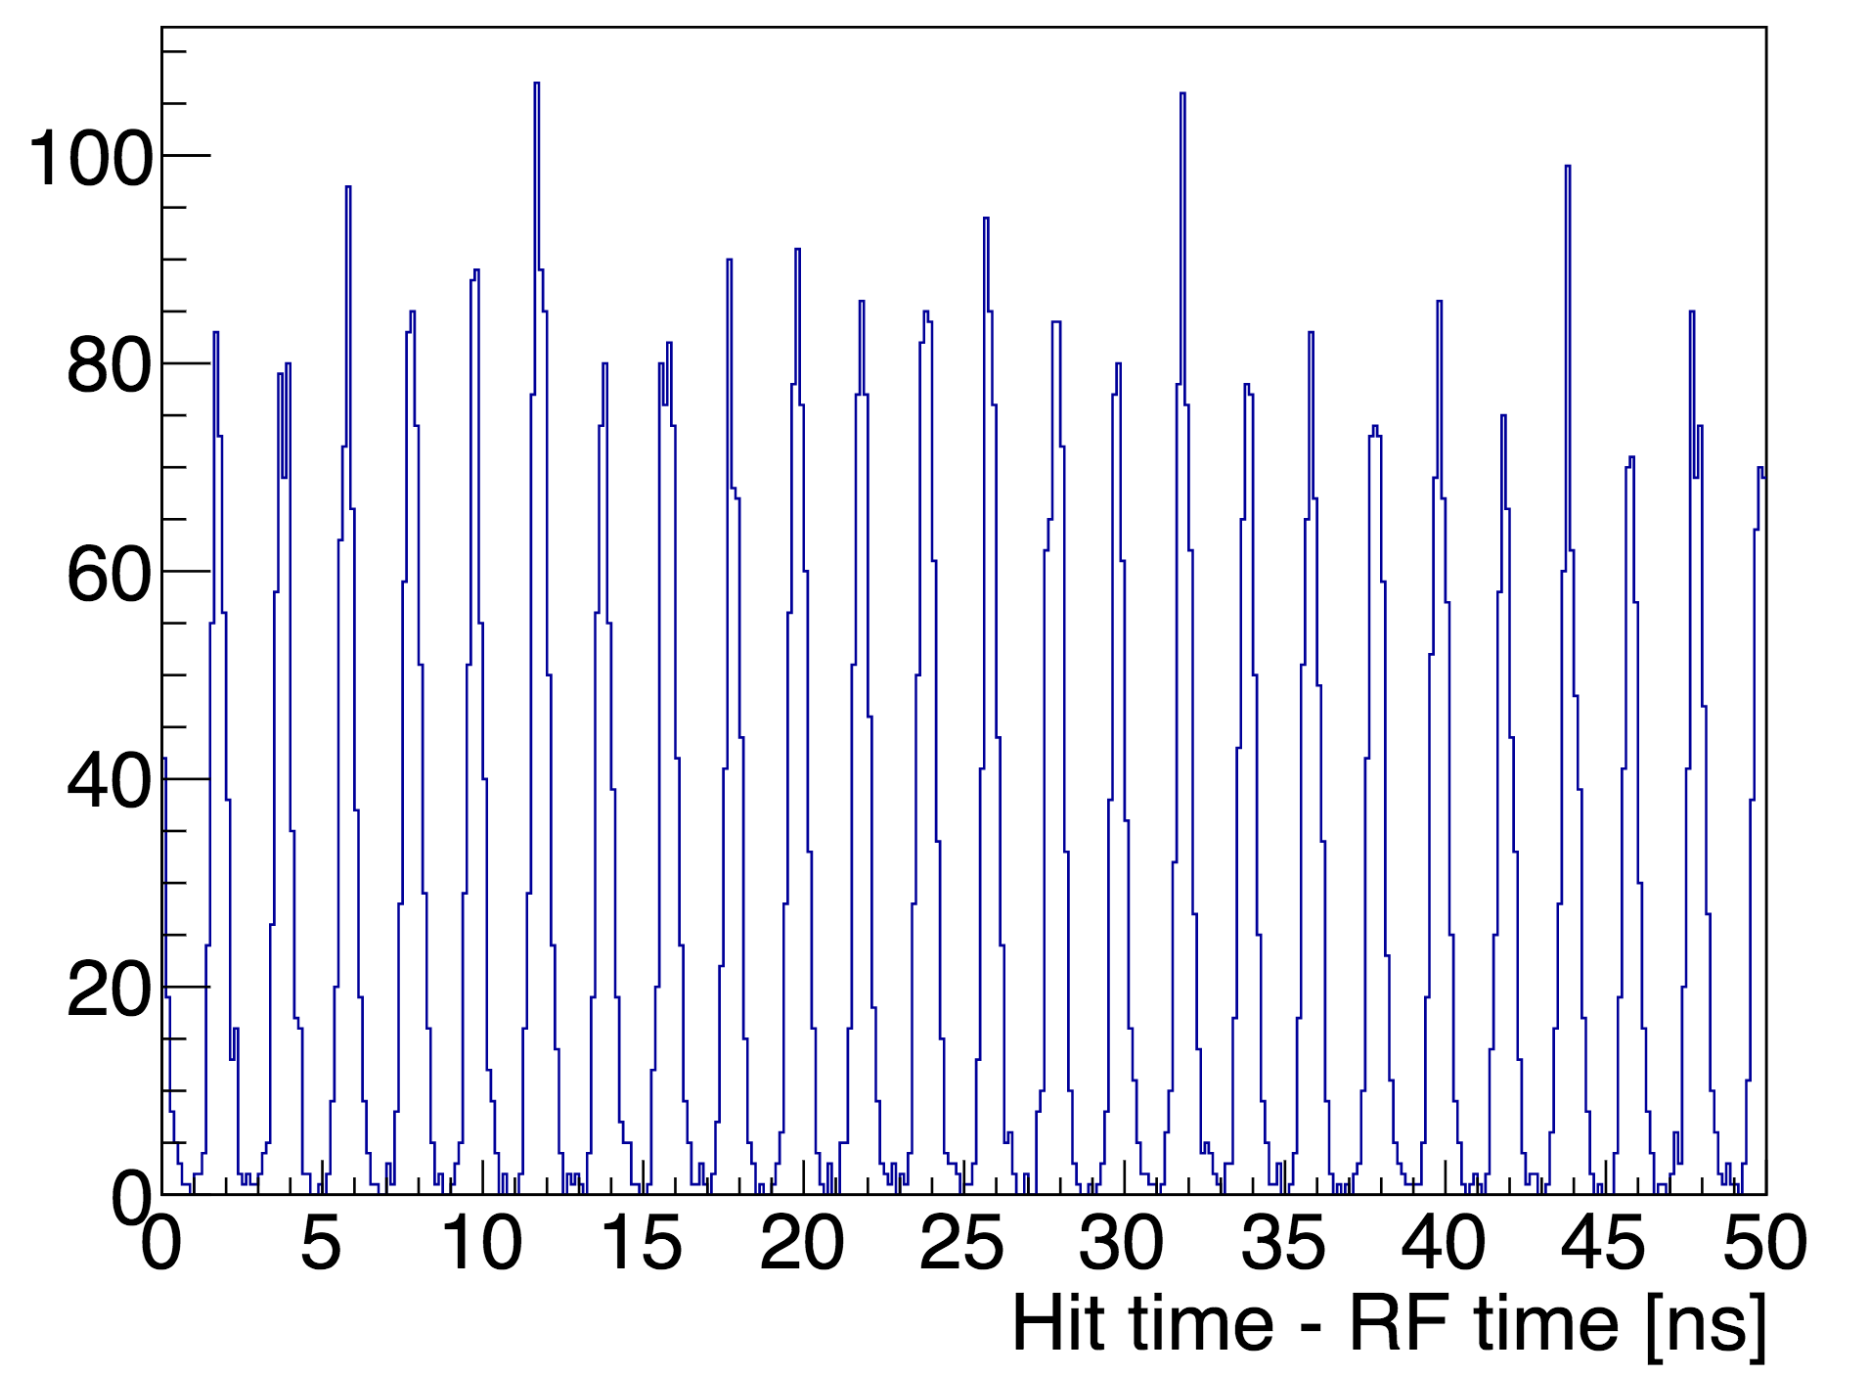
\includegraphics[width=0.7\textwidth]{pics/performance/beamStructure.png}
  \caption[Time difference between ECal hits and RF time]{From the time difference between ECal hits and the RF time, electron beam bunch structure is seen to occur at approximately 2~ns, consistent with known accelerator frequency.}
  \label{Figure:beamBunch}
\end{figure}

By applying Equation~\eqref{eq:tfine} to Figure~\ref{Figure:beamBunch}, we align all of the signals and see the fine offset of each module with respect to the RF time. This technique only shows the offset component that is less than 2~ns and results in all crystals being aligned to the nearest 2$n$~ns, where $n$ is any integer. 

To fully align the crystals, we choose a crystal to align with RF signal at 0, and then align all other crystals with respect to this crystal. Because the primary trigger for HPS is a cluster pairs trigger, we can compare the time difference between clusters to make this correction. The time of the highest energy hit in a cluster was used to set the time for the cluster. Comparison studies exploring the use of an energy-weighted cluster time using the hit times in a cluster found no significant difference due to the seed hit energy dominating the time distribution and producing the same results as if one had used the time from the seed hit only. Well-correlated pairs of clusters were selected by looking for pairs with an energy sum equal to the beam energy and an energy difference of less than 200~MeV. The times for both clusters must have occurred in the 30-70~ns time window for the Engineering Run which was the optimal time window for triggered events. The time difference correction between two pairs of clusters after the fine time offset correction is shown in Figure~\ref{Figure:2clusoffset}.

\begin{figure}[H]
  \centering
      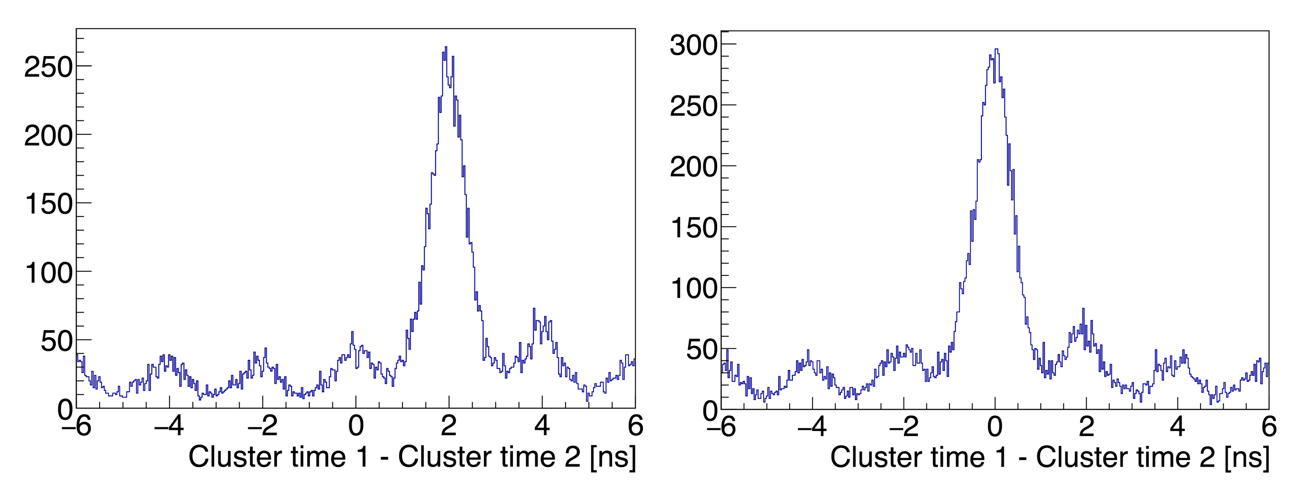
\includegraphics[width=0.9\textwidth]{pics/performance/2clusteroffset.png}
  \caption[Time difference between two clusters after fine offset time correction]{After correcting all clusters with the fine timing offset correction, clusters are aligned to the nearest 2~ns time offset with respect to the RF signal. Shown on the left is a cluster pair that has an overall 2~ns time difference that needs to be accounted for in the final offset with the RF time. The plot on the right shows a different cluster pair with an offset centered at 0.}
  \label{Figure:2clusoffset}
\end{figure}

In Figure~\ref{Figure:2clusoffset}, a large 2~ns offset between a cluster pair is seen on the left prior to this step in the timing correction with respect to the RF signal. A different cluster pair, shown on the right, is seen to have no overall time offset that needs to be accounted for with respect to the RF time. \\
\indent After correcting for the time offsets of all crystals with respect to the RF time, an energy-dependent correction, known as the time walk correction, must be accounted for. Time walk is the time difference of a signal crossing threshold in an ADC due to the finite rise time of the leading edge and the difference in signal amplitudes for particles of different energies. The effect causes particles of lower energy to cross the threshold later in time than particles of higher energy. This effect is not physical and can be removed by studying the time difference between hits in a cluster versus the seed hit as a function of the hit energy. Pulse fitting of the raw signal removes most of the time walk when compared to other methods that can be used to obtain a hit time. In the Engineering Run data, the seed hit was greater than 400 MeV and provided a reasonable threshold against which to compare hit times at lower energies. For the Physics Run data, the time walk correction was able to use a much higher seed hit threshold of 1~GeV, and the energy-dependence could be extended to higher energies. The time walk can be extracted from the comparison of the the hit times within a cluster as shown in Figure~\ref{Figure:hittimeincluster}.

\begin{figure}[H]
  \centering
      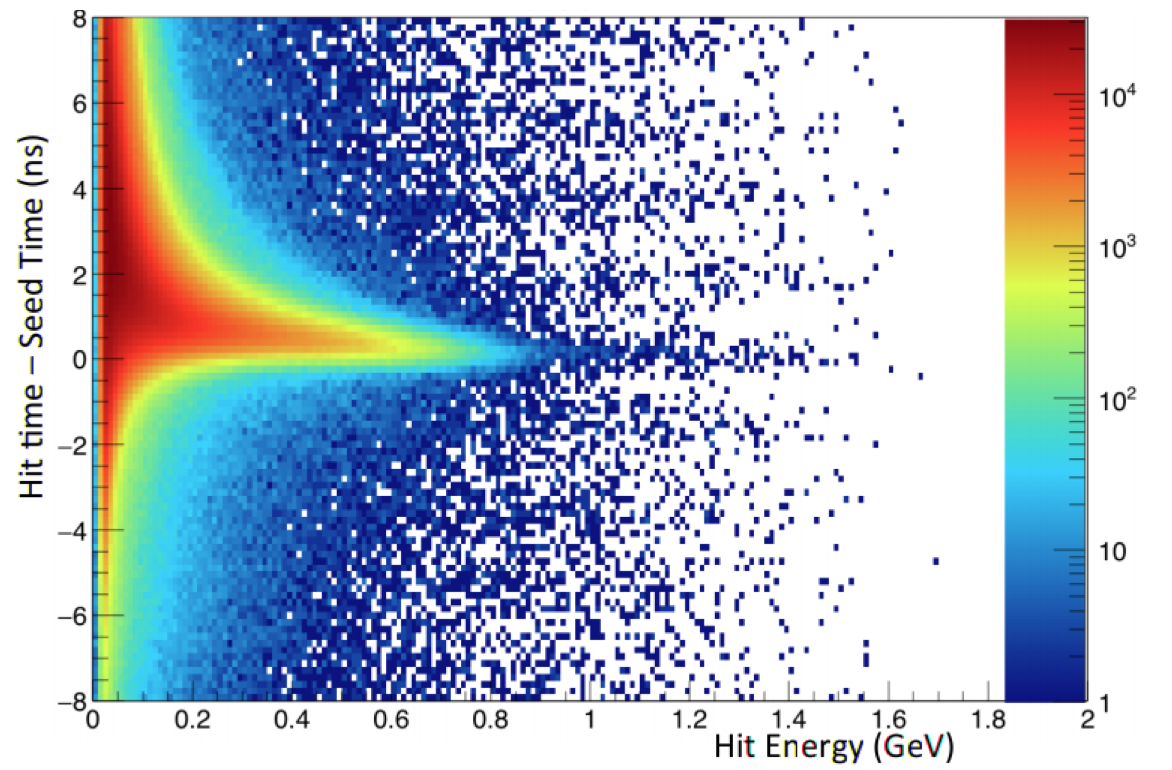
\includegraphics[width=0.7\textwidth]{pics/performance/hittimeincluster.png}
  \caption[Hit times in a cluster versus the hit energy]{The time walk correction for the 2016 data can be extracted from the difference of hit times in a cluster versus the seed hit time as a function of the the hit energy.}
  \label{Figure:hittimeincluster}
\end{figure}

The time walk correction found from the Physics Run data is shown in Figure~\ref{Figure:twalk}. 

\begin{figure}[H]
  \centering
      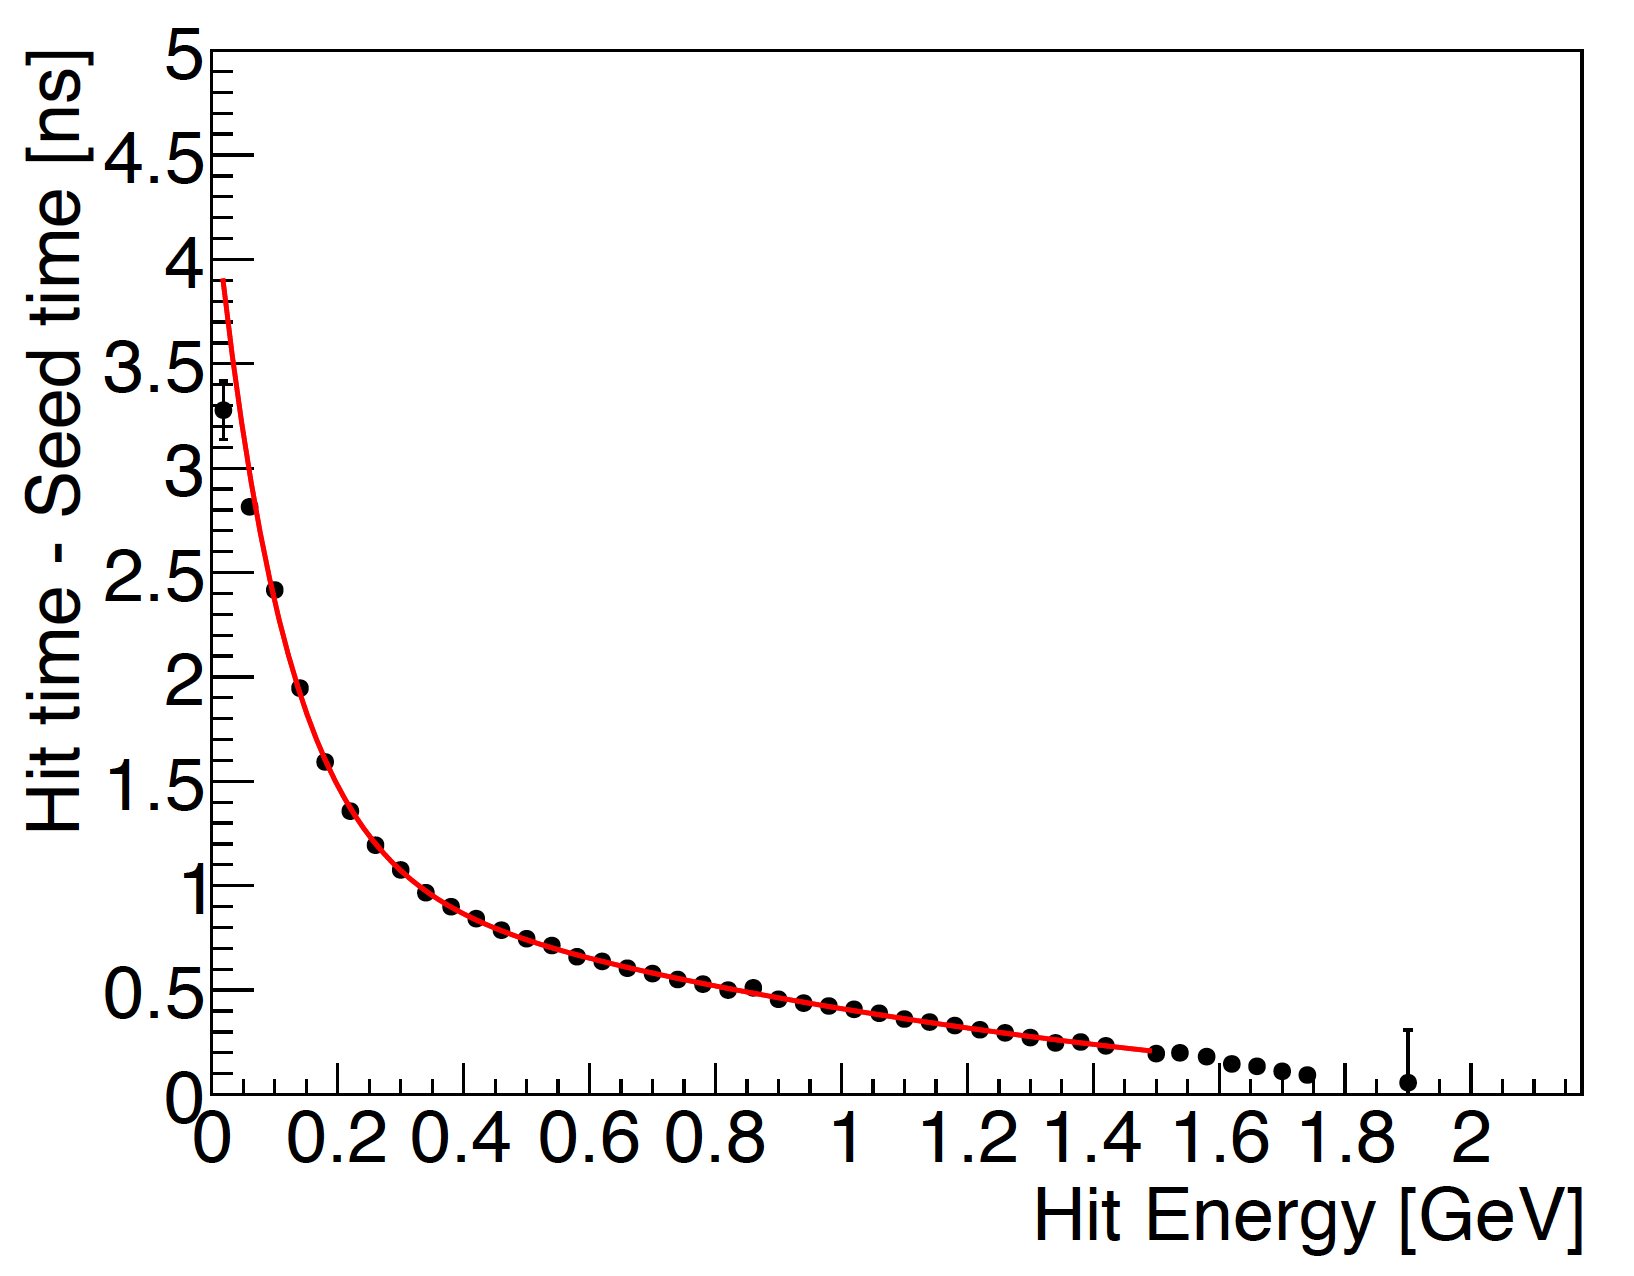
\includegraphics[width=0.6\textwidth]{pics/performance/twalk2016.png}
  \caption[Time walk correction for the Physics Run ECal data]{The time walk correction for the Physics Run data was found by comparing the time difference between hits in a cluster versus the seed hit time.}
  \label{Figure:twalk}
\end{figure}

The time walk shown in Figure~\ref{Figure:twalk} is described by the form in Equation~\eqref{eq:twalkEq}.

\begin{equation}
	\label{eq:twalkEq}
		\Delta_{t_{walk}} = e^{p_0+p_1E}+p_2+p_3E+p_4E^2	
\end{equation}

After removing all crystal-to-crystal time offsets and applying the energy-dependent time walk correction to all modules, the resulting time resolution for all energies is shown in Figure~\ref{Figure:timeRes}. 

\begin{figure}[H]
  \centering
      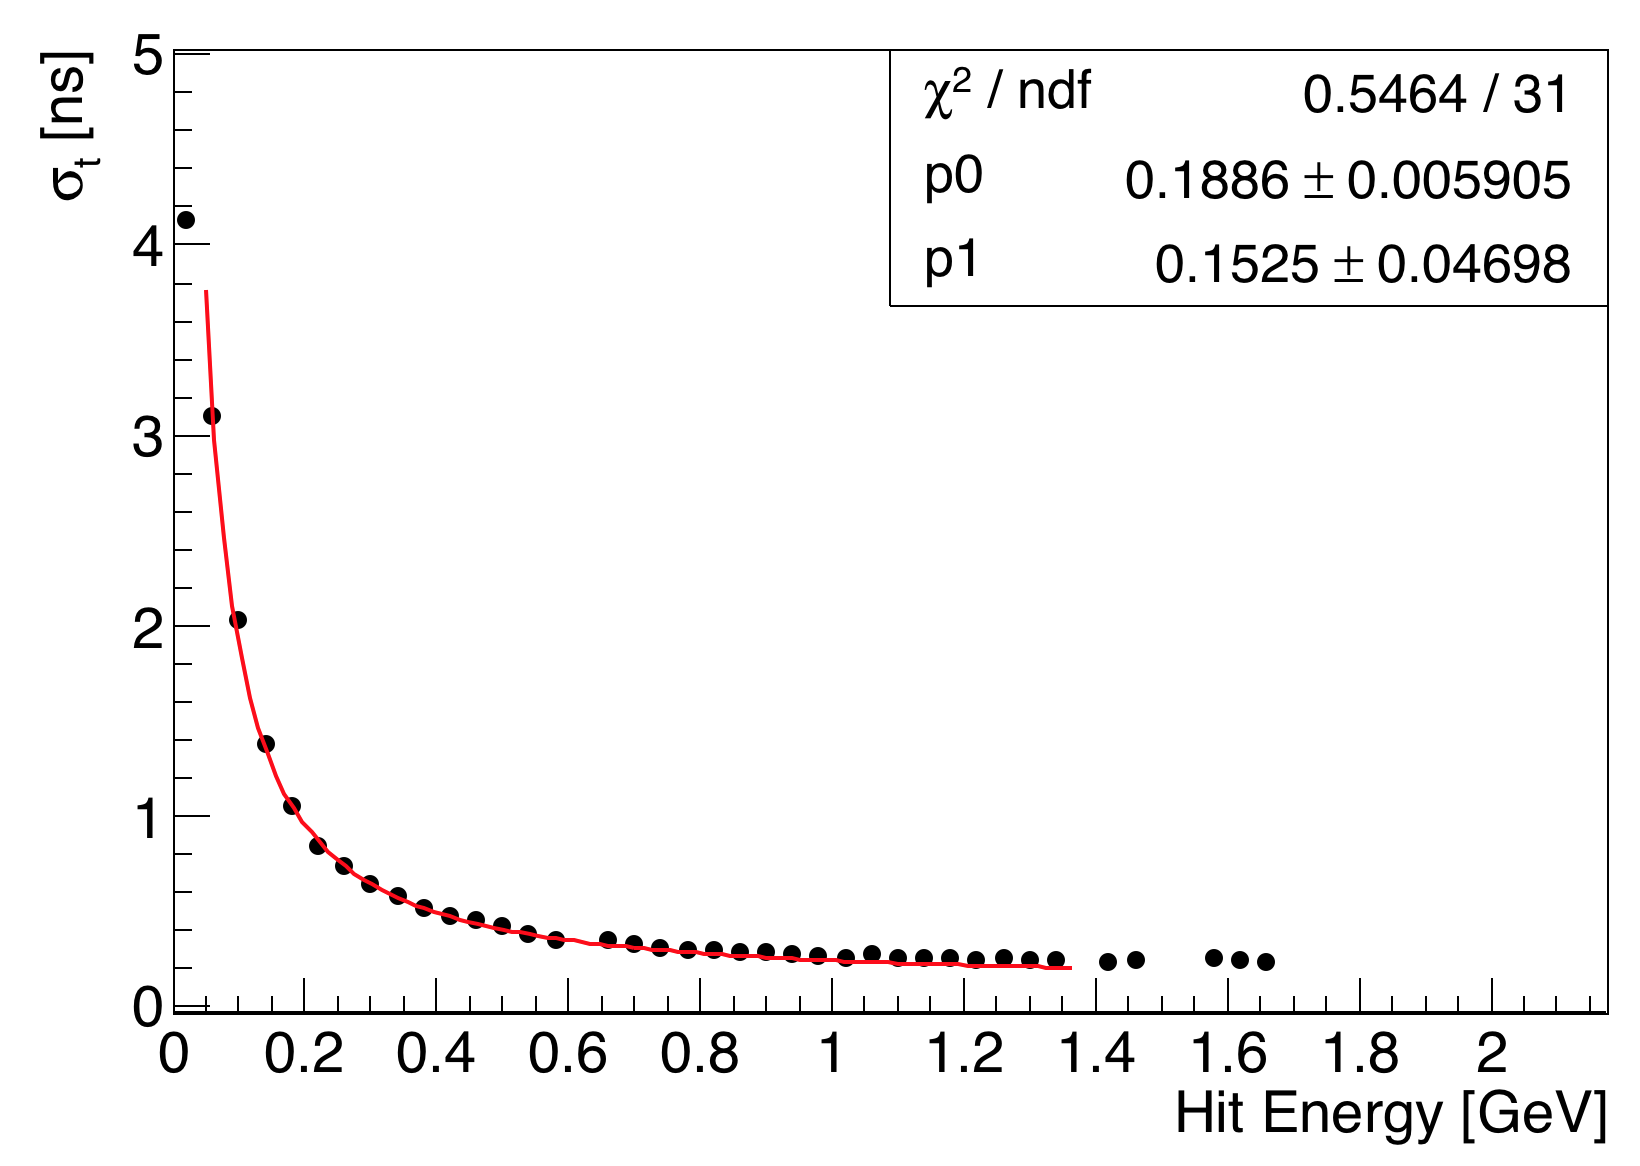
\includegraphics[width=0.6\textwidth]{pics/performance/timeRes2016.png}
  \caption[Time resolution of the ECal for the 2016 run ]{The time resolution as a function of energy is shown.}
  \label{Figure:timeRes}
\end{figure}

The time resolution as a function of hit energy shown in Figure~\ref{Figure:timeRes} is described by Equation~\eqref{Figure:twalkEqn}

\begin{equation}
	\label{eq:twalkEqn}
		\sigma_t \textsf{ [ns]} = \dfrac{p0}{E}\oplus p1	
\end{equation}

The measured time resolution for the time difference between two clusters is shown in Figure~\ref{Figure:timeRes2cl}.

\begin{figure}[H]
  \centering
      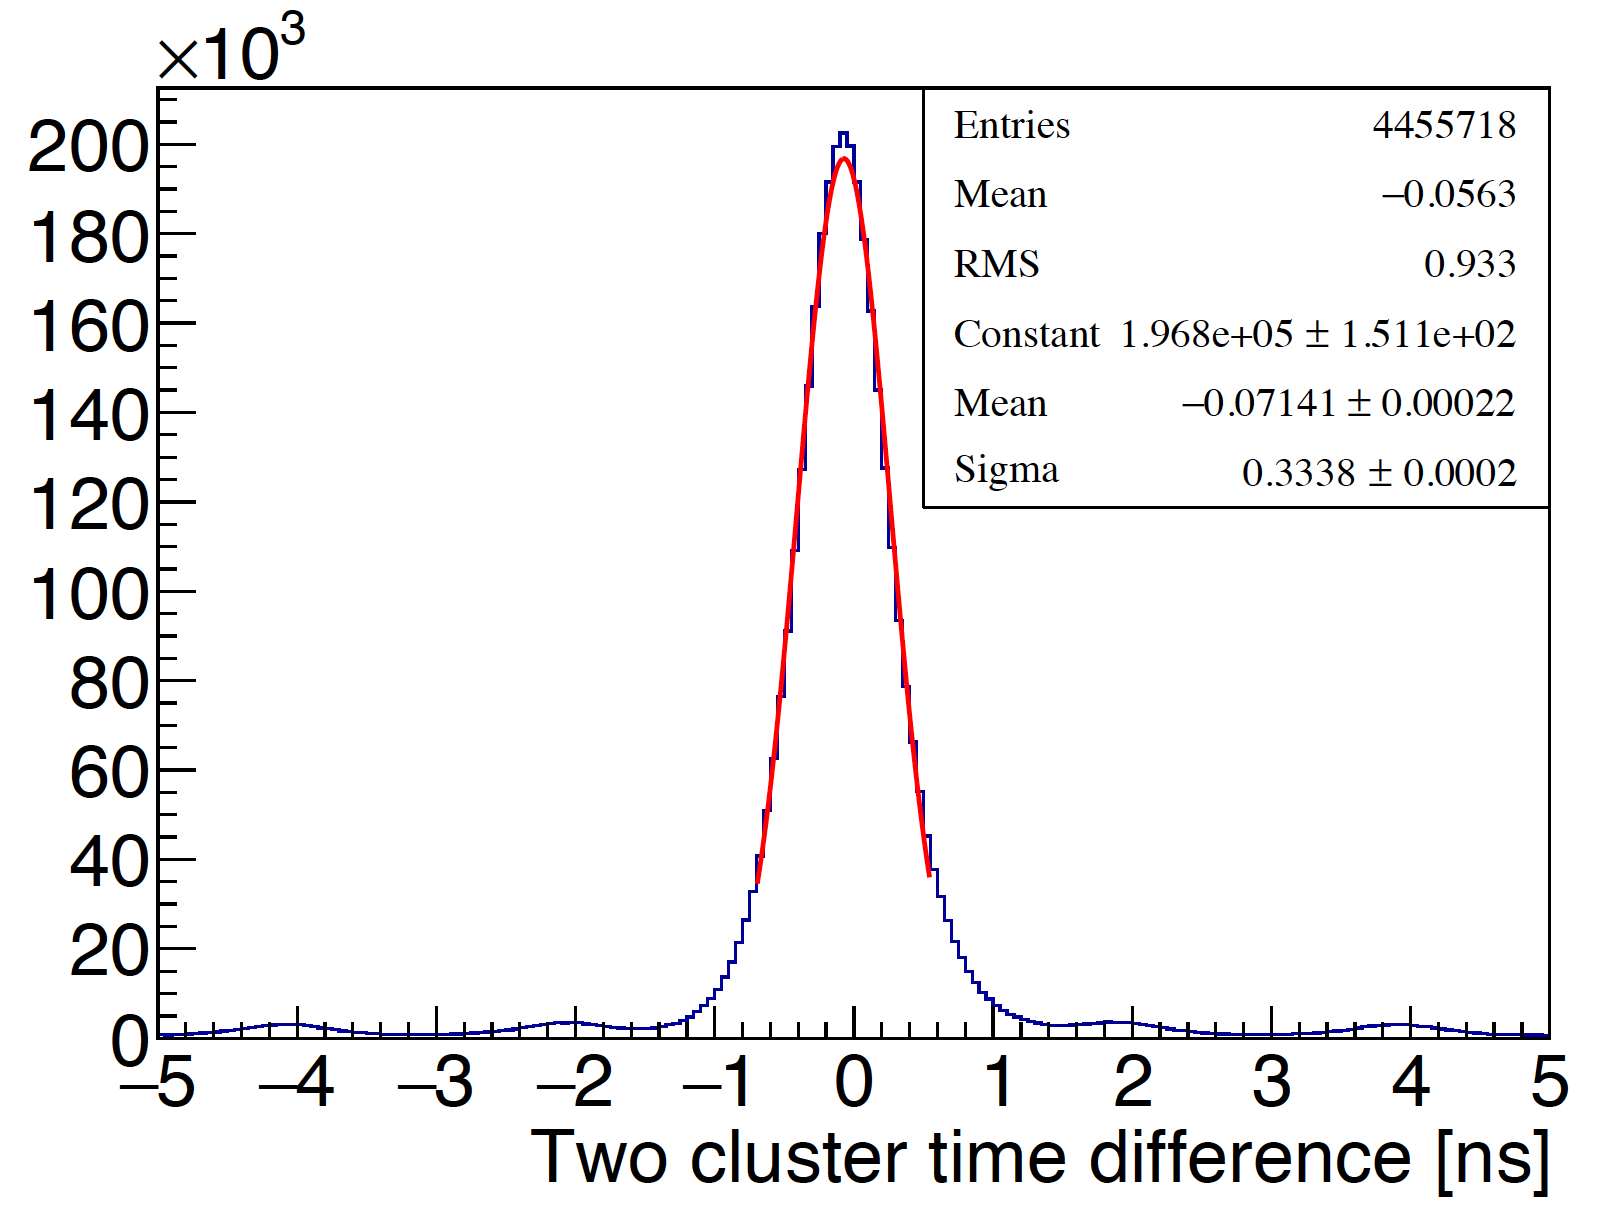
\includegraphics[width=0.6\textwidth]{pics/performance/2clusterTres.png}
  \caption[Time resolution for the time difference between two clusters]{The time difference between two clusters is shown. The energies sum to greater than 80$\%$ of the beam energy and have a resulting resolution of approximately 330~ps .}
  \label{Figure:timeRes2cl}
\end{figure}

As shown in Figure~\ref{Figure:timeRes2cl}, for two clusters that have an energy sum greater than 80$\%$ the beam energy in 2016, the resolution is approximately 330~ps. For the Engineering Run at a lower beam energy, the resolution of the time difference between two clusters was found to be approximately 470~ps. 

%%%%%%%%%%%%%%%%%%%%%%%%%%%%%%%%%%%%%%%%%
\chapter{Searching for displaced vertices}
The events relevant to the vertex analysis were triggered using the pairs-1 HPS trigger cuts. The data is loosely selected as pairs that have a cluster in the top and bottom of the ECal. A radiative cut, a cut on the measured sum of the energy of the two reconstructed particles in order to selected $A^{\prime}$ events of interest, is chosen to greater than 80$\%$ of the beam energy. Tracks are reconstructed using various methods and a Generalized Broken Lines (GBL) track re-fit is performed using a minimum of five hits in a track. A vertex is constructed using an unconstrained vertex fit meaning that the closest approach of an $e^+e^-$ track pair is used to construct the vertex. While the beam spot constrained vertex collection was not used for measuring vertex position of a pair, the $\chi^{2}$ of the beam spot constrained vertex fit described the quality of how closely the two tracks pass each other in addition to how well the total momentum projects back to the beam spot position at the target. 
\indent The beam spot constrained collection is not used as the primary collection for studying the vertex position because the beam spot position at the target is not precisely known. If using the z vertex position from a beam spot constrained fit, the size of the beam spot weights the significance of the beam spot as a factor in the vertex fit. A bad beam spot position can systematically pull the measured vertex position. For genuine $A^{\prime}$ displaced vertices, the z vertex position  is relatively unchanged when using a beam spot vs an unconstrained vertex fit. For identifying backgrounds, prompt vertices that are pushed to large z through measurement error, the beamspot constraint can arbitrarily bias the location of the scattered vertex. In order to avoid bias to the reconstructed z vertex position, the unconstrained fit is used.  \\
\indent The tracks are projected to the ECal and matched to clusters based on position and momentum. There exists an established parameterization of the track-cluster matching that can be used to measure the quality of the match as a a count of standard deviation, $n\sigma$. Furthermore, the ECal has a superior timing resolution to the SVT and the time difference between two clusters can be used to study both accidentals and elimination of tracks originating from different events. \\
\indent There are a few cuts that originate specifically from studies of high z background events and physics processes which include cuts on the positron track's distance of closest approach in the $XZ$ plane to the target (DOCA), the $e^+e^-$ momenutm asymmetry, and the number of hits shared between tracks. 

\section{Datasets}
%%TODO: input final reach numbers
During the Engineering Run, the beam energy was 1.056~GeV, and a total of 1.7~days (1166~nb$^{-1}$) of data-taking was achieved with the SVT at the nominal position where Layer 1 is at $\pm$0.5~mm from the beam. An additional 0.47~days (362.7~nb$^{-1}$) was achieved, prior to moving the SVT to the nominal position, with the SVT Layer 1 at $\pm$1.5~mm from the beam. A large portion of the data taken with the first layer of the SVT at $\pm$1.5~mm was unable to be used due to an incorrect timing latency in the SVT DAQ and is excluded from this analysis. There are a total of six datasets as shown in Table~\ref{tab:datasets}.

\begin{table}[htb]
\caption{Vertexing Datasets}
\label{tab:datasets}
\centering
\begin{tabular}{lllr}
\toprule
%\multicolumn{2}{c}{Name} \\
%\cmidrule(r){1-2}
Datasets &First hit of track & SVT position & statistics \\
\midrule
L1L1 & Both tracks layer 1 & 0.5~mm & 13,697,082\\
L1L2 & One track layer 1 & 0.5~mm & 302,103\\
L2L2 & Both tracks layer 2 & 0.5~mm & 4,876\\
L1L1 & Both tracks layer 1 & 1.5~mm & 1,635,172\\
L1L2 & One track layer 1 & 1.5~mm & 1,005,668\\
L2L2 & Both tracks layer 2 & 1.5~mm & 233,388\\
\bottomrule
\end{tabular}
\end{table}

The backgrounds, statistics, efficiencies and $zCut$s are different for each dataset, and therefore require separate analyses before combining the limits of the final results of each. The datasets are determined by the first hit layer of the $e^+e^-$ tracks that makeup the vertex. Each dataset is exclusive of the other datasets. When one hit misses Layer 1, a fiducial cut to exclude the active region of Layer 1 is used on the extrapolated track position to Layer 1 in order to ensure that the Layer 1 inefficiencies, which are still currently not completely understood, do not inflate the statistics of the dataset. 

\section{$A^{\prime}$ signal in the displaced vertex search}
%change out fit for 100% l1l1 slice
We must select a downstream region for which to look for a heavy photon having virtually no background. Therefore, we choose a $zCut$ which is a downstream z vertex position beyond which there is less than 0.5~background event/bin. We arbitrarily choose our maximum z value, $zMax$, to be at the first layer, although this can vary depending on the dataset. The $zCut$ varies as a function of mass and can be ideally selected to minimize backgrounds whilst maximizing A' production. The number of events we can expect to reconstruct is described by Equation~\eqref{eq:signal}.

\begin{equation}
\label{eq:signal}
S_{bin,zCut} = \left( \dfrac{N_{rad}}{N_{tot}}\right) N_{bin}\left(\dfrac{3\pi\epsilon^{2}}{2N_{eff}\alpha}\right)\left(\dfrac{m_{A'}}{\delta m_{A'}}\right)\epsilon_{bin}\int_{zCut}^{zMax}\dfrac{e^{-ztgt-z/\gamma c\tau}}{\gamma c \tau}\epsilon_{vtx}(z,m_{A'})dz
\end{equation}

In Equation~\eqref{eq:signal}, the heavy photon production at the target per mass bin is described by the first four terms. $\epsilon_{bin}$ is chosen as the fraction of signal we reconstruct within our selected mass bin window(we choose a mass window of $\pm1.4\sigma_m$ corresponding to an $\epsilon_{bin}$ of 0.838). The $N_{rad}/N_{tot}$ is the radiative fraction which is the fraction of radiatives contained in the sample and is derived from Monte Carlo. The $N_{bin}$ is the number of measured e+e- pairs at a given mass. The third and fourth terms are what was explained in Equation~\eqref{eq:crossSection}. The integral calculates the number of heavy photons we could reconstruct in the decay region from $zCut$ to $zMax$, where $z=0$ is the target location. $\epsilon_{vtx}$ represents the efficiency of detecting $e+e-$ pairs from an A' of mass $m_{A'}$ that decayed at position $z$ from the target and is inclusive of the efficiencies of all other cuts used in the analysis. Based on Poisson statistics, the 90$\%$ confidence limit for a null result requires to have an expected number of A' events as defined in Equation~\ref{eq:signal} to be greater than 2.303.\\
\indent In order to find the value of $zCut$, we slice the distribution of the reconstructed vertex position versus reconstructed mass in bins of mass and fit the core of the vertex distribution with a Gaussian with the normal parameters of $\sigma$ and $z_{mean}$ while fitting the downstream tail of the distribution with an exponential. The fit for the full vertex distribution per mass bin is described by Equation~\eqref{eq:vtxFit}.

\begin{equation}
\label{eq:vtxFit}
\begin{split}
F(z < b) & =  Ae^{-\dfrac{(z-z_{mean})^2}{2\sigma^2}}\\
F(z > b) & =  Ae^{-\dfrac{b^2}{2\sigma^2}-\dfrac{z-z_{mean}-b}{l}}
\end{split}
\end{equation}

As shown in Equation~\eqref{eq:vtxFit}, there is an additional parameter $b$ which defines the distance from the core of the Gaussian that the fit will be described by the exponential tail. The exponential tail, where $z>b$, is defined in terms of the parameter $l$, controlling the length of the tail, and describes the downstream tail of the vertex distribution. The $zCut$ is selected from this function where there remains 0.5 background events downstream. A fit to a mass slice from the L1L1 dataset is shown in Figure~\ref{fig:vtxFitPic}.

\begin{figure}[htb]
  \centering
      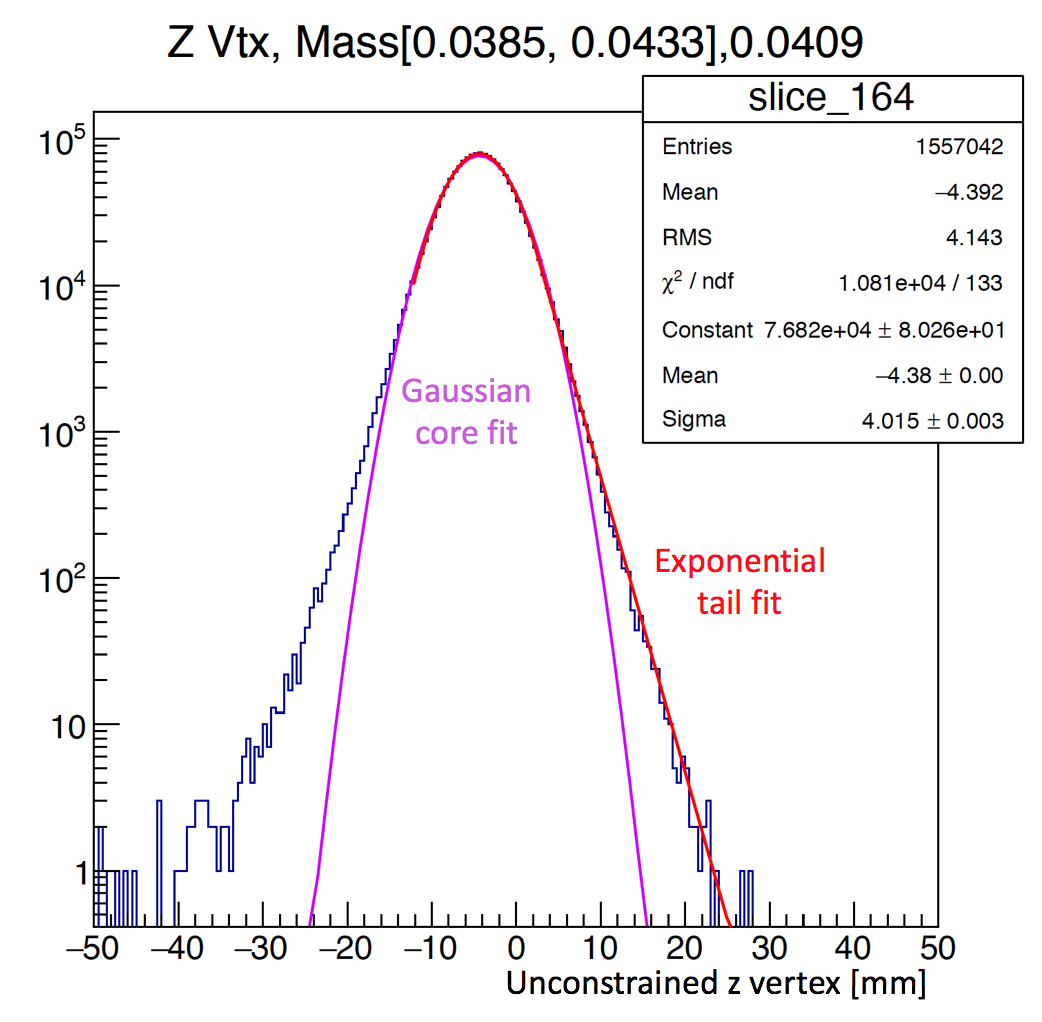
\includegraphics[width=0.7\textwidth]{pics/searching/vtxFit.png}
  \caption[Fit to vertex slice at a mass of 41~MeV]{For a mass slice centered at 41~MeV, the vertex distribution in the full L1L1 dataset is shown and fitted. The fit functions are described by Equation~\eqref{eq:vtxFit} where the core of the distribution is fit with a Gaussian and the downstream tail is fit with an exponential.}
  \label{fig:vtxFitPic}
\end{figure} 



\section{Monte Carlo simulation}
Background events can be produced from QED trident processes and wide-angle bremsstrahlung (WAB). The trident processes can be separated into "radiative" and "Bethe-Heitler" diagrams. In particular, the heavy photon production is related to the radiative trident cross section. The $A^{\prime}$ production for a mass bin is described as shown in Equation~\eqref{eq:crossSection}.

\begin{equation}
\label{eq:crossSection}
\dfrac{d\sigma(A'\rightarrow e+e-)}{d\sigma(\gamma*\rightarrow e+e-)} = \left(\dfrac{3\pi\epsilon^{2}}{2N_{eff}\alpha}\right)\left(\dfrac{m_{A'}}{\delta m_{A'}}\right)
\end{equation}

In Equation~\eqref{eq:crossSection}, $N_{eff}$, the number of available decay states, is one for the HPS experiment which explores a mass range in which the heavy photon can only decay to one Standard Model final state ($e+e-$). The $\epsilon^{2}$ refers to the coupling factor between the heavy photon and the Standard Model while the $\alpha$ is the fine structure constant. The $\dfrac{m_{A'}}{\delta_{m_{A'}}}$ refers to the central mass value considered in the mass bin of study. After accounting for all backgrounds, prior to the radiative cut to the data at 80$\%$ of the beam energy, the energy sum of the two particles is in general agreement between Monte Carlo and data as shown in Figure~\ref{fig:mcAgree}.

\begin{figure}[htb]
  \centering
      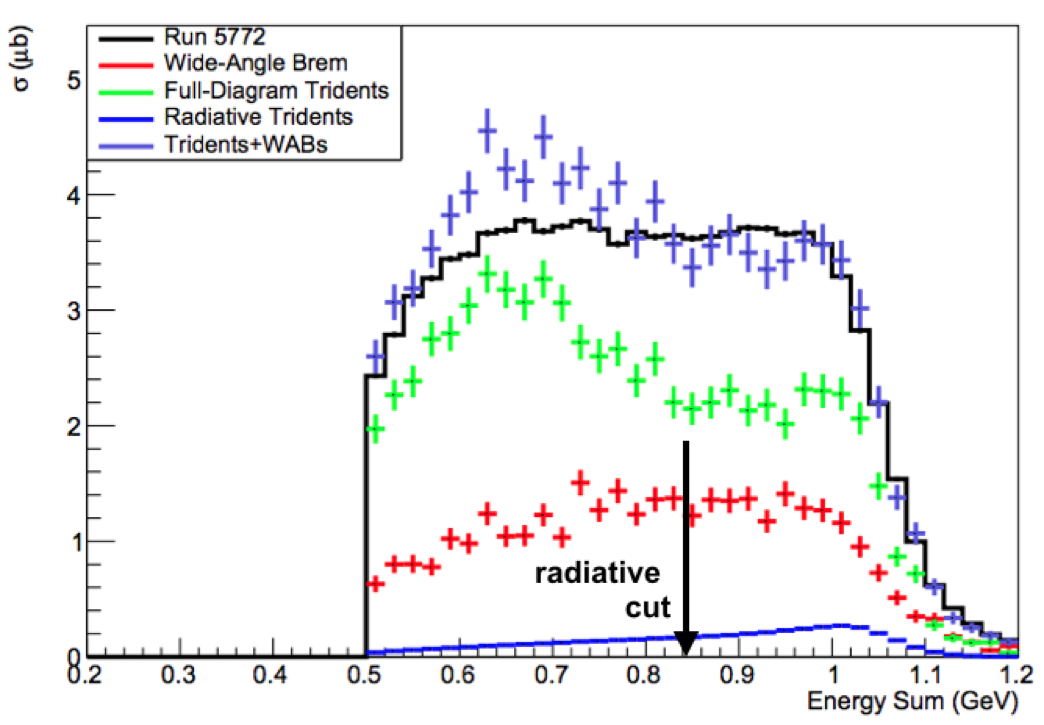
\includegraphics[width=0.8\textwidth]{pics/searching/mcAgree.png}
  \caption[Energy sum comparison in Monte Carlo and data]{Energy sum in Monte Carlo and data. The energy sum is in general agreement at the high end of the spectrum where HPS is optimized to search for heavy photons. Further studies to isolate track and SVT layer inefficiencies at the lower energy sum are still being explored.}
  \label{fig:mcAgree}
\end{figure} 

The fraction of radiative reactions amongst trident events in the HPS search region is the radiative fraction. Using MadGraph5 Monte Carlo to model the tridents and radiatives and MadGraph4 Monte Carlo to model the wide angle bremsstrahlung (WAB) background, the radiative fraction can be determined as shown in Figure~\ref{fig:radFrac}.

\begin{figure}[htb]
  \centering
      \includegraphics[width=0.9\textwidth]{pics/searching/radFrac.png}
  \caption[Radiative fraction from Monte Carlo]{Radiative fraction using MadGraph5 Monte Carlo and spinfix WAB.}
  \label{fig:radFrac}
\end{figure} 

As shown in Figure~\ref{fig:radFrac}, the radiative fraction relevant to the vertex analysis is approximately 9.5$\%$ for all masses. This fraction is defined as the ratio of radiative events to the background events (tritrig+WAB in Figure~\ref{fig:radFrac}) and is the same for both the 0.5~mm and 1.5~mm data sets.


\subsection{Vertex reconstruction efficiencies, $\epsilon_{vtx}$}
The integral described in Equation~\eqref{eq:signal} contains an $\epsilon_{vtx}$ parameter that describes the number of events we can reconstruct beyond the $zCut$ and includes both detector acceptance and inefficiencies. Using A' Monte Carlo, $\epsilon_{vtx}$ is calculated and the efficiency is parameterized as a function of mass and $z$ vertex position. At each mass, the ratio of the reconstructed to generated heavy photon events is scaled such that for L1L1, the fitted ratio is 1 at that target position. The reconstruction efficiency at the target without scaling is shown in Figure~\ref{fig:rawEff}.

\begin{figure}[H]
  \centering
      \includegraphics[width=0.8\textwidth]{pics/searching/rawEffL1L1.png}
  \caption[Reconstruction efficiency for heavy photons that decay at the target]{Reconstruction efficiency for heavy photon events with decay vertices at the target as a function of mass.}
  \label{fig:rawEff}
\end{figure} 

As shown in Figure~\ref{fig:rawEff}, the maximum efficiency in the HPS detector for events that decay promptly occurs around heavy photon masses between 40-50~MeV. This reconstruction efficiency at the target is normalized to 1, and the L1L2 and L2L2 data sets are scaled to ensure the same relative relationship between the three data sets. The reconstruction efficiencies for a 35~MeV heavy photon as a function of position are shown in Figure~\ref{fig:apEff}. 

\begin{figure}[H]
  \centering
      \includegraphics[width=0.8\textwidth]{pics/searching/reconstructedVtx.png}
  \caption[Fraction of reconstructed events of a 35~MeV A$^{\prime}$ as a function of decay vertex position]{Fraction of reconstructed events of a 35~MeV A$^{\prime}$ as a function of decay vertex position. The three datasets are mutually exclusive. Each data set is fit independently of the others and parameterized in terms of mass and $z$ vertex position. }
  \label{fig:apEff}
\end{figure} 

As shown in Figure~\ref{fig:apEff}, as all data sets are mutually exclusive of each other, the total reconstruction efficiency for all z vertex positions is the sum of the efficiencies for the individual datasets. These efficiencies are then integrated from different $zCut$ values to $zMax$ (roughly set at the z position of Layer 1, or 10~cm). The efficiency at each mass for each data set is fitted with a corresponding functional description that is parameterized in terms of mass and $z$ vertex position. The vertex reconstruction efficiency for the L1L1 data is described by Equation~\eqref{eq:promptfunction}.

\begin{equation}
\label{eq:promptfunction}
\epsilon_{vtx} = exp(p_0+p_1z+p_2z^2+p_3z^3) 
\end{equation}

In Equation~\eqref{eq:promptfunction}, all parameters are functions of mass. For the L1L2 data, the reconstruction efficiency turns on farther downstream and is described by a Crystal Ball function as shown in Equation~\eqref{eq:cbfunction}.

\begin{eqnarray*}
\label{eq:cbfunction}
\epsilon_{vtx}(t >= -| \alpha |) & = & N e^{-0.5t^{2}}\\
\epsilon_{vtx}(t < -| \alpha |) & = & N A(B-t)^{-n}\\
\textsf{where:}\\
\alpha & = & 0.97\\
n & = & 141.5\\
t & = & \dfrac{z-z_{mean}}{\sigma}\\
A & = & (\dfrac{n}{| \alpha |})^{n}e^{-0.5 |\alpha |^2}\\
B & = & \dfrac{n}{| \alpha |}-|\alpha | \\
N & = & \textsf{amplitude of the Gaussian}
\end{eqnarray*}

From Equation~\eqref{eq:cbfunction}, the parameters $z_{mean}$, $\sigma$, and $N$ are obtained from fitting the distribution and are functions of mass. The L2L2 data set efficiency turns on farther downstream than L1L2 and is best described by a Gaussian as in Equation~\eqref{eq:gausfunction}.

\begin{equation}
\label{eq:gausfunction}
Ne^{-0.5\dfrac{(z-z_{mean})^2}{\sigma^2}}
\end{equation}

The individual fit parameter values are described numerically in ~\ref{appendix:vtxEff}.\\
\indent Once these relations are derived, we obtain a value for $\epsilon_{vtx}$ that is integrated from the $zCut$ to the maximum $zMax$ when calculating the expected signal yield. The full integral is shown in Figure~\ref{fig:effIntegral} as the color z-axis and is a function of both the heavy photon mass and $zCut$.  

\begin{figure}[H]
  \centering
      \includegraphics[width=0.8\textwidth]{pics/searching/integralEffL1L1.png}
  \caption[Integral as a function of mass and $zCut$ for L1L1]{The z-axis shows the color corresponding to the integral value for the L1L1 0.5~mm data set as a function of the $zCut$ and mass. The coupling, $\epsilon^2$ is fixed here to $5E-9$ and $zMax$ is chosen to be 10~cm, corresponding to the $z$ position of the first SVT layer. }
  \label{fig:effIntegral}
\end{figure}

The full integral value yields some fractional number that, when multiplied by the expected heavy photon yield from the cross section, tells us how many heavy photons we can expect to reconstruct in the given decay vertex region. For the L1L1 dataset, it is critical to set the zCut as low as possible in order to obtain the highest signal yield. In Figure~\ref{fig:effIntegral}, the value of the integral indicated by the color on the z-axis, is shown for $\epsilon^{2} = 5E-9$ as a function of mass and $zCut$. The $zMax$ was set to 10~cm in this calculation. The same calculation is done for the L1L2 dataset at shown in Figure~\ref{fig:effIntegral12}.

\begin{figure}[H]
  \centering
      \includegraphics[width=0.8\textwidth]{pics/searching/integralEff12.png}
  \caption[Integral as a function of mass and $zCut$ for L1L2]{The z-axis shows the color corresponding to the integral value for the L1L2 0.5~mm data set as a function of the $zCut$ and mass. The coupling, $\epsilon^2$ is fixed here to $5E-9$ and $zMax$ is chosen to be 10~cm, corresponding to the $z$ position of the first SVT layer. }
  \label{fig:effIntegral12}
\end{figure}

In Figure~\ref{fig:effIntegral12}, the maximum fractional signal yield is significantly less than in the L1L1 data set. The lifetime of the heavy photon in Figure~\ref{fig:effIntegral12} is not long enough to significantly benefit from the additional efficiency obtained at longer displaced $z$ vertex positions. The integrated efficiency for the L2L2 data is shown in Figure~\ref{fig:effIntegral22}.

\begin{figure}[H]
  \centering
      \includegraphics[width=0.8\textwidth]{pics/searching/integralEff22.png}
  \caption[Integral as a function of mass and $zCut$ for L2L2]{The z-axis shows the color corresponding to the integral value for the L2L2 0.5~mm data set as a function of the $zCut$ and mass. The coupling, $\epsilon^2$ is fixed here to $5E-9$ and $zMax$ is chosen to be 10~cm, corresponding to the $z$ position of the first SVT layer. }
  \label{fig:effIntegral22}
\end{figure}

As shown in Figure~\ref{fig:effIntegral22}, the fraction yield is significantly less when compared to the L1L1 dataset and requires a very small $zCut$ value in order to recover the maximum yield. Additionally, the L1L2 and L2L2 datasets are most beneficial for detecting lower mass A$^\prime$s with displaced $z$ vertex positions. 

\subsection{Mass resolution}
It was previously observed that the mass resolution in Monte Carlo deteriorated for displaced vertices. The problem arises due to the track parameters not being adjusted for the vertex position~\cite{billoir_fast_1992}. A correction to the measured mass is defined as shown in Figure~\ref{eq:massCorrection}.

\begin{equation}
\label{eq:massCorrection}
m_{corr} = m_{uc} - \dfrac{0.15\times 10^{-3}\times z_{vtx}}{m_{uc}}(\dfrac{P_{x,e-}}{P_{e-}}-\dfrac{P_{x,e+}}{P_{e+}})            
\end{equation}

In Equation~\eqref{eq:massCorrection}, the unconstrained vertex mass is $m_{uc}$, the reconstructed $z$ vertex position downstream is $z_{vtx}$, the horizontal momentum component is indicated by $P_x$ where the corresponding particle type is also indicated by the subscript, and the magnitude of the momentum is $P$. The effects of the correction to the reconstructed mass can be seen in Figure~\ref{fig:effectMCorr}.

\begin{figure}[htb]
  \centering
      \includegraphics[width=0.9\textwidth]{pics/searching/massCorrection.png}
  \caption[Correction to the reconstructed mass for a 40~MeV $A^{\prime}$]{The mass residual of a reconstructed 40~MeV $A^{\prime}$ is shown as a function of vertex position in $z$. The uncorrected mass residual as given from the vertexer is shown on the left. The resolution deteriorates with the downstream $z$ position of the vertex. After the correction is applied, as shown on the right, the mass resolution is no longer vertex position dependent.}
  \label{fig:effectMCorr}
\end{figure} 

The mass resolution is determined from $A^{\prime}$ Monte Carlo and has been checked with the $e^-e^-$ mass resolution from M\o ller scattered electron pairs in data. By generating heavy photons at discrete masses, applying the cuts proposed in data, and fitting the $A^{\prime}$ mass peak residual with respect to the generated mass peak, the mass resolution can be measured as a function of mass. A fit to the generated 40~MeV heavy photon in Monte Carlo is shown in Figure~\ref{fig:ap40mev}.

\begin{figure}[htb]
  \centering
      \includegraphics[width=0.65\textwidth]{pics/searching/ap40mev.png}
  \caption[Fit to the mass residual of a 40~MeV $A^{\prime}$]{The residual of a reconstructed 40~MeV $A^{\prime}$ mass is shown with a Gaussian fit.}
  \label{fig:ap40mev}
\end{figure} 

Simulations of the M\o ller mass can be used to study systematic offsets between the measured mass resolution in data and the mass resolution found in Monte Carlo. Using M\o ller Monte Carlo (with no beam background), the M\o ller mass can be seen in Figure~\ref{fig:mollerMC}. 

\begin{figure}[htb]
  \centering
      \includegraphics[width=0.65\textwidth]{pics/searching/mollerMassMC.png}
  \caption[Fit to the M\o ller mass peak in Monte Carlo]{The M\o ller mass peak from Monte Carlo with a Crystal Ball fit is shown. The background is fit with a Gaussian.}
  \label{fig:mollerMC}
\end{figure} 

The M\o ller mass from Monte Carlo can be immediately compared with the M\o ller mass found in data. The difference in resolution between the peak from the pure Monte Carlo M\o ller sample and the M\o ller sample in data is approximately 17$\%$. This difference should be applied to the heavy photon mass resolution found in Monte Carlo in order to appropriately scale the bin widths when slicing and fitting the vertex distribution by mass. The M\o ller peak from data is shown in Figure~\ref{fig:mollerMass}. 

\begin{figure}[htb]
  \centering
      \includegraphics[width=0.65\textwidth]{pics/searching/mollerMass.png}
  \caption[Fit to the M\o ller mass peak in data]{The M\o ller mass peak with a Crystal Ball fit in data is shown.The low mass background on the front of the peak is fit with a Gaussian.}
  \label{fig:mollerMass}
\end{figure} 

The mass resolution is shown on Figure~\ref{fig:massRes} as a function of mass.

\begin{figure}[htb]
  \centering
      \includegraphics[width=0.65\textwidth]{pics/searching/massResolution.png}
  \caption[Mass resolution compared between Monte Carlo and data]{The mass resolution is compared here between Monte Carlo and data. The mass resolution points shown in blue measure the residual of the reconstructed mass in heavy photon Monte Carlo. The mass resolution shown in purple is from the fit to the M\o ller mass peak when reconstructed in Monte Carlo. The green point is the M\o ller mass resolution as measured in data. The difference between the Monte Carlo and data M\o ller mass resolutions is approximately 17$\%$. This scaling should be applied to the linear fit $0.02082m+0.0006$ from Monte Carlo in order to account for the difference in resolution.}
  \label{fig:massRes}
\end{figure} 

After applying the 17$\%$ scaling to the mass resolution from A' Monte Carlo, we obtain the mass resolution in Equation~\eqref{eq:massresScaled}.

\begin{equation}
\label{eq:massresScaled}
\sigma_m = 0.02082m+0.0007
\end{equation}

The scaled mass resolution in Equation~\eqref{eq:massresScaled} is used in the vertex analysis to find the $z$ vertex cut. 





%\section{Combining Ecal and SVT measurements}

\section{Vertex cuts}
\input{texFiles/Searching/blindCuts.tex}
\subsection{Cuts after unblinding}
Discuss the additional cuts after unblinding: L2 isolation to all sets, matching, track chi2/dof, kink cuts
%\input{texFiles/Searching/unblindCuts.tex}
%\section{Combined reach projections}

The total reach of all 0.5~mm data only is shown in Figure~\ref{fig:reach0p5only}.

\begin{figure}[H]
  \centering
     \includegraphics[width=0.8\textwidth]{plots/reachall_0p5.png}
  \caption{The expected signal yield for the full 100$\%$ dataset with all 0.5~mm data.}
  \label{fig:reach0p5only}
\end{figure} 

The reach as shown in Figure~\ref{fig:reach0p5only} uses the projected zCut for 100$\%$ of the data and assumes that we can optimize and use the L2L2 dataset. Using the same assumptions, we can obtain the reach for the 1.5~mm dataset alone in Figure~\ref{fig:reach1p5only}.

\begin{figure}[H]
  \centering
     \includegraphics[width=0.8\textwidth]{plots/reachall_1p5.png}
  \caption{The expected signal yield for the full 100$\%$ dataset with all 1.5~mm data.}
  \label{fig:reach1p5only}
\end{figure} 

By combining the reach of the 0.5~mm and 1.5~mm datasets, we obtain the full upper limit of the reach we can expect when we unblind the full 2015 data as shown in Figure~\ref{fig:reachall}.

\begin{figure}[H]
  \centering
     \includegraphics[width=0.8\textwidth]{plots/reachall.png}
  \caption{The expected signal yield for the full 100$\%$ dataset with 0.5~mm and 1.5~mm data combined.}
  \label{fig:reachall}
\end{figure} 

While the statistics of the 0.5~mm dataset drive the reach, the various settings of the SVT and different layer requirements can contribute to the reach by probing the parameter space in different regions of mass and coupling. The maximum signal in  Figure~\ref{fig:reachall} is 0.39~events. In order to have obtained any reach with the data, it would have been necessary to run an additional six times longer than what we did. 
\indent The contributions from the L2L2 datasets are upper limit estimates that require improved mass resolution and removal of high z backgrounds. 


\section{Calculating zCut}
Discuss the z vs mass distributions with zCut and accidentals for the 10$\%$ sample.

%%%%%%%%%%%%%%%%%%%%%%%%%%%%%%%%%%%%%%%%%
\chapter{Vertex Search Results} 
Show full data set z vs mass distribution with zCut. 


\section{Characterizing the background}
Discuss quantiles, look elsewhere effect, p-values


\subsection{SVT at nominal position}
\subsection{SVT at open position}
\subsection{Estimate of contamination by accidentals}

\section{Reach}




%%%%%%%%%%%%%%%%%%%%%%%%%%%%%%%%%%%%%%%%%
\chapter{Conclusion}


%\begin{thebibliography}{99}

\bibliography{biblio}{}
\bibliographystyle{unsrt}
%\printbibliography
  %This begins the list of reference or bibliography. The default form is consistent
  %with the references in the Physical Review. The articles must be listed in the order
  %in which they appear in the text. The style of the bibliography can be changed and
  %automatic ordering of the entries can be accomplished using BibTeX. Use of BibTeX is
  %explained in most of the standard LaTeX books. Using BibTeX has the advantage that the
  %entries in the bibliography will be properly ordered automatically.  It is also makes
  %hyperlinking to the bibliography entries to citations in the text and to publisher's
  %sites that allow quick access to the cited material.
  
%\addtocontents{toc}{\vspace*{12pt}}  %This command adds some extra space in the table of
                                     %contents
\addcontentsline{toc}{chapter}{BIBLIOGRAPHY}  %This command adds and entry for the
                                              %bibliography in the table of contents
                                              

%\end{thebibliography}

%This command begins the Appendix section. The style of the chapter numbering is changed to
%letters

\appendix


%A new command for appendix chapters has been defined called \achapter that has been modified
%so that it can add the appendices to the table of contents in the approved form.

\achapter{Vertex reconstruction efficiencies}
\label{appendix:vtxEff}
The 0.5~mm reconstructed vertex efficiency, $\epsilon_{vtx}$ is described by the following parameterizations. For the L1L1 dataset fit by Equation~\eqref{eq:promptfunction}, the parameters are shown in Equation~\ref{eq:parsEpsVtxL1}.

\begin{eqnarray*}
\label{eq:parsEpsVtxL1}
p_0 & = & -0.2359+3.606m\\
p_1 & = & -0.03537+0.5395m \\
p_2 & = & -0.001201+0.1404m-2.614m^2+10.65m^3 \\
p_3 & = & -0.0002078+0.008753m-0.1396m^2+0.8077m^3\\
\end{eqnarray*}

For the L1L2 dataset with the SVT at 0.5~mm from the beam, the parameters fit to Equation~\eqref{eq:cbfunction} are described by Equation~\eqref{eq:parsEpsVtxL1L2}.

\begin{eqnarray*}
\label{eq:parsEpsVtxL1L2}
z_{mean} & = & -58.89+5208.95m-76469.9m^2+386631m^3\\
\sigma & = & 3.05+629.99m-14691.8m^2+114123m^3\\
N & = & -0.3125+37.0172m-472.052m^2 \\
\end{eqnarray*}

For the L2L2 dataset with the SVT at 0.5~mm from the beam, the parameters fit to Equation~\eqref{eq:gausfunction} are described by Equation~\eqref{eq:parsEpsVtxL2L2}.

\begin{eqnarray*}
\label{eq:parsEpsVtxL2L2}
N & = & -0.3623+30.88m-374.7m^2\\
z_{mean} & = & -71.7603+7733.51m-131569m^2+827080m^3\\
\sigma & = & -4.058-813m-8947m^2\\
\end{eqnarray*}


%include 1.5mm efficiency equations here
The 1.5~mm reconstructed vertex efficiency, $\epsilon_{vtx}$ is described by the following parameterizations. For the L1L1 dataset fit by Equation~\eqref{eq:promptfunction}, the parameters are shown in Equation~\ref{eq:parsEpsVtxL1O}.

\begin{eqnarray*}
\label{eq:parsEpsVtxL1O}
p_0 & = & (m<0.029)\times(194.3m-5.9590)+(x\geq 0.029)\times(4.937m-0.3635)\\
p_1 & = & (x<0.032)\times(19.52m-0.6578)+(x\geq 0.032)\times(-9.889m^2+1.928m-0.09032)\\
p_2 & = & -0.01753+0.8977m-13.89m^2+65.14m^3 \\
p_3 & = & (x<0.0285)\times(0.3299m-0.009391)+(x\geq 0.0285)\times(0.001647m-0.0001239)\\
\end{eqnarray*}

For the L1L2 dataset with the SVT at 1.5~mm from the beam, the parameters fit to Equation~\eqref{eq:cbfunction} are described by Equation~\eqref{eq:parsEpsVtxL1L2O}.

\begin{eqnarray*}
\label{eq:parsEpsVtxL1L2O}
z_{mean} & = & -72.7326+4494.67m-40308.4m^2\\
\sigma & = & 7.7148+79.5054m\\
N & = & -0.3178+22.8208m-253.373m^2 \\
\end{eqnarray*}

For the L2L2 dataset with the SVT at 1.5~mm from the beam, the parameters fit to Equation~\eqref{eq:gausfunction} are described by Equation~\eqref{eq:parsEpsVtxL2L2O}.

\begin{eqnarray*}
\label{eq:parsEpsVtxL2L2O}
N & = & -0.3623+30.8816m-374.691m^2\\
z_{mean} & = & -71.6658+7732.18m-131207m^2+823016m^3\\
\sigma & = & -8.9366+1109.97m-13284.4m^2\\
\end{eqnarray*}


\achapter{Vertex analysis cuts}
\label{appendix:vtxCuts}
\subsection{L1L2 with SVT at 0.5 mm}

The L1L2 data set with the SVT at the nominal 0.5~mm position consists of tracks where the one track missed the active region of Layer 1. This data set combines the case for which the electron passes through Layer 1 and the positron passes through Layer 1 in order to obtaining the $zCut$ because it was noted that the tails of the distributions are the same (despite the known backgrounds being different and could merit improved cuts that would divide the data set in the future). \\
\indent The cuts applied to the L1L2 data set are shown in Table~\ref{l1l2_cuts}. 

\begin{table}[H]
\caption{Cuts applied to the L1L2 datasets.}
\label{l1l2_cuts}
\centering
\begin{tabular}{lllllll}
\toprule
%\multicolumn{2}{c}{Name} \\
%\cmidrule(r){1-2}
Cut type & Cut & Cut Value &  $\%$killed &  $\%$killed core & $\%$killed tails\\
\midrule
track & Fit quality & track $\chi^{2}<30$ & 38 & 15 & 47 \\
track & Max track momentum &  $P_{trk}<75\%E_{beam}$ & 12 & 8 & 14 \\
track & Isolation &   & 11 & 4 & 15 \\
vertex & beamspot constraint & bsc$\chi^{2}<10$  & 46 & 24 & 60 \\
vertex & beamspot - unconstrained & bsc$\chi^{2}$-unc$\chi^2<5$  & 20 & 16 & 24 \\
vertex & maximum $P_{sum}$ &  $<115\%E_{beam}$ & 1 & 1 & 1 \\
ecal & Ecal SVT matching & $\chi^2<10$  & 7 & 7 & 8 \\
ecal & track Ecal timing & $<4$ns  & 5 & 5 & 5 \\
ecal & 2 cluster time diff & $<2$ns  & 8 & 6 & 10 \\
physics & momentum asymmetry & $<0.4$  & 14 & 15 & 13 \\
physics & e+ track d0 & $<1.5$mm  & 7 & 3 & 11 \\
event & max shared hits amongst tracks & $<5$ shared hits  & 8 & 7 & 8 \\
track & cuts on kink tails & $\phi$ and $\lambda$ kink tails & 19 & 9 & 36 \\
\bottomrule
\end{tabular}
\end{table}

The initial selection requires that a track that missed Layer 1 has a projection to the z location at layer 1 that is less than 1.5~mm from the beam. This ensures that the sample is not overly contaminated by events that passed through the active region but failed to identify a hit. As a result, the core of the distribution sits on the downstream side of the z-axis and reflects the geometric constraints we have imposed. The first cut that is different from the L1L1 data set is the isolation cut. In this data set, we apply the same isolation cut to the track that passed through Layer 1, but we apply a slightly different isolation cut for the track that did not pass through layer 1. The isolation in layer 2 is measured and projected to the target position to be compared with the impact parameter of the track in $y$ at the target. Additional cuts are applied to the tails of the kink distributions for the tracks. The summary of these cuts is made in the Table~\ref{kink_cuts}.

\begin{table}[H]
\caption{Cuts applied to the kinks in layers 1-3.}
\label{kink_cuts}
\centering
\begin{tabular}{lll}
\toprule
%\multicolumn{2}{c}{Name} \\
%\cmidrule(r){1-2}
Cut & Value \\
\midrule
Layer 1: $\phi$ kink, $\lambda$ kink & <0.0001,<0.002\\
Layer 2: $\phi$ kink, $\lambda$ kink & <0.002,<0.004\\
Layer 3: $\phi$ kink, $\lambda$ kink & <0.002,<0.004\\
\bottomrule
\end{tabular}
\end{table}

The uncut kink distributions for the electron with the cut indicated by the red dashed line is shown in Figures~\ref{fig:kink1}, \ref{fig:kink2}, and \ref{fig:kink3}.

\begin{figure}[H]
  \centering
      \includegraphics[width=0.8\textwidth]{pics/appendix/kink1.png}
  \caption{The kink distributions for tracks passing through Layer 1. The cut is shown at the red dashed line.}
  \label{fig:kink1}
\end{figure} 
\begin{figure}[H]
  \centering
      \includegraphics[width=0.8\textwidth]{pics/appendix/kink2.png}
  \caption{The kink distributions for tracks passing through Layer 2. The cut is shown at the red dashed line.}
  \label{fig:kink2}
\end{figure} 
\begin{figure}[H]
  \centering
      \includegraphics[width=0.8\textwidth]{pics/appendix/kink3.png}
  \caption{The kink distributions for tracks passing through Layer 3. The cut is shown at the red dashed line.}
  \label{fig:kink3}
\end{figure} 

The positron kink distributions look similar to the electron kink distributions and are not shown here. These cuts remove events from the tails. The effects of all the cuts on the reconstructed vertex position distribution are shown in Figure~\ref{fig:zvtxCuts_l1l2}.

\begin{figure}[H]
  \centering
      \includegraphics[width=0.8\textwidth]{pics/appendix/zvtxCuts_L1L2.png}
  \caption{The effects of the cuts on the L1L2 dataset on the unconstrained z vertex.}
  \label{fig:zvtxCuts_l1l2}
\end{figure} 

The effects of the cuts on the reconstructed mass distribution are shown in Figure~\ref{fig:massCuts_l1l2}.

\begin{figure}[H]
  \centering
      \includegraphics[width=0.8\textwidth]{pics/appendix/massCuts_L1L2.png}
  \caption{The effects of the cuts on the L1L2 dataset on the mass distribution.}
  \label{fig:massCuts_l1l2}
\end{figure} 

This dataset has the tendency to contain more WAB contamination than the L1L1 dataset. In particular, we know from Monte Carlo that positrons are unlikely to have a hit in Layer 1 when the photon in WAB pair produces after the target. Additionally, this sample contains a 5:1 ratio of having in electron versus a positron in the first layer. 

\subsection{L2L2 with SVT at 0.5 mm}

The L2L2 dataset consists of vertices produced when tracks do not pass through Layer 1 and their projections back to Layer 1 are within 1.5~mm of the beam (outside the active silicon region). This dataset requires the most work to remove the background events, and preliminary studies with the small number of statistics have been unsuccessful. \\
\indent The general cuts applied to the L2L2 dataset, after first requiring that track projections do not extend to the active region of Layer 1, are listed in Table~\ref{l2l2_cuts}.

\begin{table}[H]
\caption{Cuts applied to the L2L2 datasets.}
\label{l2l2_cuts}
\centering
\begin{tabular}{lllllll}
\toprule
%\multicolumn{2}{c}{Name} \\
%\cmidrule(r){1-2}
Cut type & Cut & Cut Value &  $\%$killed &  $\%$killed core & $\%$killed tails\\
\midrule
track & Fit quality & track $\chi^{2}<30$ & 44 & 66 & 44 \\
track & Max track momentum &  $P_{trk}<75\%E_{beam}$ & 15 & 14 & 15 \\
track & Isolation &   & 22 & 34 & 22 \\
vertex & beamspot constraint & bsc$\chi^{2}<10$  & 47 & 36 & 47 \\
vertex & beamspot - unconstrained & bsc$\chi^{2}$-unc$\chi^2<5$  & 18 & 0 & 19 \\
vertex & maximum $P_{sum}$ &  $<115\%E_{beam}$ & 1 & 6 & 1 \\
ecal & Ecal SVT matching & $\chi^2<10$  & 30 & 73 & 29 \\
ecal & track Ecal timing & $<4$ns  & 7 & 0 & 8 \\
ecal & 2 cluster time diff & $<2$ns  & 8 & 0 & 8 \\
physics & momentum asymmetry & $<0.4$  & 4 & 0 & 4 \\
physics & e+ track d0 & $<1.5$mm  & 21 & 33 & 21 \\
event & max shared hits amongst tracks & $<4$ shared hits  & 21 & 50 & 21 \\
\bottomrule
\end{tabular}
\end{table}

The geometric acceptance of the cuts in the L2L2 data set leave a core fraction of background events well beyond the target at approximately 30~mm downstream. The only modifications to previously applied cuts are that both tracks use a modified isolation cut by looking at the isolation at Layer 2 and the tracks do not share 4 hits with any other track in the event.  The kink cuts appeared to not remove events from this data set.

\subsection{L1L1 with SVT at 1.5 mm}
The L1L1 dataset in the 1.5~mm data includes vertices reconstructed from pairs of tracks that have hits in Layer 1 of the SVT. Due to the SVT opening being larger, the acceptance favors larger heavy photon masses. The SVT has also lower rates in Layer 1 when compared to the 0.5~mm dataset.\\
\indent The cuts applied to the L1L1 dataset are shown in Table~\ref{l1l1_cuts_1p5}.

\begin{table}[H]
\caption{Cuts applied to the L1L1 datasets with the SVT at 1.5mm.}
\label{l1l1_cuts_1p5}
\centering
\begin{tabular}{llllll}
\toprule
%\multicolumn{2}{c}{Name} \\
%\cmidrule(r){1-2}
Cut type & Cut & Cut Value &  $\%$killed &  $\%$killed core & $\%$killed tails\\
\midrule
track & Fit quality & track $\chi^{2}<30$ & 37 & 22 & 87 \\
track & Max track momentum &  $P_{trk}<75\%E_{beam}$ & 6 & 6 & 19 \\
track & Isolation &   & 2 & 1 & 15 \\
vertex & beamspot constraint & bsc$\chi^{2}<10$  & 23 & 21 & 81 \\
vertex & beamspot - unconstrained & bsc$\chi^{2}$-unc$\chi^2<5$  & 12 & 12 & 27 \\
vertex & maximum $P_{sum}$ &  $<115\%E_{beam}$ & 0 & 0 & 2 \\
ecal & Ecal SVT matching & $\chi^2<10$  & 3 & 3 & 58 \\
ecal & track Ecal timing & $<4$ns  & 5 & 5 & 7 \\
ecal & 2 cluster time diff & $<2$ns  & 4 & 4 & 13 \\
physics & momentum asymmetry & $<0.4$  & 12 & 12 & 48 \\
physics & e+ track d0 & $<1.5$mm  & 0 & 0 & 4 \\
event & max shared hits amongst tracks & $<5$ shared hits  & 12 & 12 & 20 \\
\bottomrule
\end{tabular}
\end{table}

The cuts are the same as those applied to the 0.5~mm dataset with similar effect.

\subsection{L1L2 with SVT at 1.5 mm}
The following section describes the data set where one track misses Layer 1 of the SVT and its track projection back to Layer 1 is within 2.5~mm of the beam such that the track does not extrapolate to the active region of the silicon.\\
\indent The cuts applied to the L1L2 dataset with the first layer of the SVT at 1.5~mm is shown in Table~\ref{l1l2_cuts_1p5}.

\begin{table}[H]
\caption{Cuts applied to the L1L2 datasets with the SVT at 1.5~mm.}
\label{l1l2_cuts_1p5}
\centering
\begin{tabular}{lllllll}
\toprule
%\multicolumn{2}{c}{Name} \\
%\cmidrule(r){1-2}
Cut type & Cut & Cut Value &  $\%$killed &  $\%$killed core & $\%$killed tails\\
\midrule
track & Fit quality & track $\chi^{2}<30$ & 23 & 11 & 47 \\
track & Max track momentum &  $P_{trk}<75\%E_{beam}$ & 8 & 7 & 12 \\
track & Isolation &   & 4 & 2 & 10 \\
vertex & beamspot constraint & bsc$\chi^{2}<10$  & 29 & 20 & 62 \\
vertex & beamspot - unconstrained & bsc$\chi^{2}$-unc$\chi^2<5$  & 12 & 11 & 22 \\
vertex & maximum $P_{sum}$ &  $<115\%E_{beam}$ & 0 & 0 & 0 \\
ecal & Ecal SVT matching & $\chi^2<10$  & 5 & 5 & 7 \\
ecal & track Ecal timing & $<4$ns  & 5 & 5 & 5 \\
ecal & 2 cluster time diff & $<2$ns  & 6 & 5 & 9 \\
physics & momentum asymmetry & $<0.4$  & 14 & 13 & 16 \\
physics & e+ track d0 & $<1.5$mm  & 6 & 5 & 16 \\
event & max shared hits amongst tracks & $<5$ shared hits  & 6 & 6 & 6 \\
track & cuts on kink tails & $\phi$ and $\lambda$ kink tails & 22 & 8 & 74 \\
\bottomrule
\end{tabular}
\end{table}

The cuts applied to the L1L2 dataset may require a similar optimization to eliminate backgrounds as that required of the dataset for the 0.5~mm. Namely, that, it may be necessary to separate the dataset for events where the positron versus the electron is the first to leave a hit in Layer 1. For the moment, the same cuts are used as the 1.5~mm dataset has generally lower backgrounds than that seen in the 0.5~mm dataset.

\subsection{L2L2 with SVT at 1.5 mm}
The following section discusses the events having no hit in Layer 1 of the 1.5~mm dataset. An additional requirement was made that the tracks must not project back to the active region of the Layer 1 silicon in order to avoid contamination by events with the Layer 1 inefficiency. \\
\indent The cuts applied to the L2L2 dataset are shown in Table~\ref{l2l2_cuts_1p5}.

\begin{table}[H]
\caption{Cuts applied to the L2L2 datasets with the SVT at 1.5~mm.}
\label{l2l2_cuts_1p5}
\centering
\begin{tabular}{lllllll}
\toprule
%\multicolumn{2}{c}{Name} \\
%\cmidrule(r){1-2}
Cut type & Cut & Cut Value &  $\%$killed &  $\%$killed core & $\%$killed tails\\
\midrule
track & Fit quality & track $\chi^{2}<30$ & 29 & 11 & 39 \\
track & Max track momentum &  $P_{trk}<75\%E_{beam}$ & 10 & 8 & 12 \\
track & Isolation &   & 5 & 2 & 8 \\
vertex & beamspot constraint & bsc$\chi^{2}<10$  & 26 & 16 & 35 \\
vertex & beamspot - unconstrained & bsc$\chi^{2}$-unc$\chi^2<5$  & 10 & 8 & 14 \\
vertex & maximum $P_{sum}$ &  $<115\%E_{beam}$ & 1 & 1 & 1 \\
ecal & Ecal SVT matching & $\chi^2<10$  & 11 & 8 & 14 \\
ecal & track Ecal timing & $<4$ns  & 6 & 6 & 6 \\
ecal & 2 cluster time diff & $<2$ns  & 7 & 6 & 7 \\
physics & momentum asymmetry & $<0.4$  & 3 & 2 & 4 \\
physics & e+ track d0 & $<1.5$mm  & 9 & 7 & 12 \\
event & max shared hits amongst tracks & $<4$ shared hits  & 20 & 20 & 20 \\
\bottomrule
\end{tabular}
\end{table}

The cuts are the same as those applied to the data in the 0.5~mm L2L2 dataset. This dataset has significantly more statistics that needs to be studied and may complement the analysis on the 0.5~mm high z background data. 

\achapter{Reach from other datasets}
\label{appendix:reach}
%\begin{figure}[hbt]
\begin{minipage}{0.5\textwidth}
 \includegraphics[width=\textwidth]{pics/appendix/zVm_L1L2_0p5_bl.png}
\end{minipage}\hfill\begin{minipage}{0.5\textwidth}
 \includegraphics[width=\textwidth]{pics/appendix/zVm_L1L2_0p5_ub.png}
 \end{minipage}
  \caption[$z$ vertex and mass distribution for the L1L2 data set with the SVT at $\pm0.5$~mm]{The unconstrained $z$ vertex position for the L1L2 data set with the SVT at $\pm0.5$~mm is shown as a function of the corrected mass of the $e^+e^-$ pair where one track has a hit in Layer 1 and the other track does not pass through the active region of Layer 1. The $zCut$ as measured for this data is shown in red and corresponds to the full 100$\%$ data set where there is less than 0.5 background event beyond. The projected $zCut$ from the 10$\%$ of the data is shown in magenta. The relevant mass range used to measure $zCut$ is from 0.02--0.06~GeV based on measured statistics. The 10$\%$ sample for tuning cuts is shown on the left, and the full 100$\%$ of the data is shown on the right.}
  \label{fig:zvm_l1l2}
\end{figure}
\begin{figure}[htb]
  \centering
      \includegraphics[width=0.5\textwidth]{pics/appendix/reachL1L2_0p5.png}
  \caption[Expected detectable $A^{\prime}$ signal yield from the L1L2 data at 0.5~mm.]{The expected number of detectable $A^{\prime}$ signal events from the L1L2 data set with the SVT at $\pm0.5$~mm is 0.04 events, and the distribution for coupling and mass space is shown. This calculation uses the $zCut$ shown in Figure~\ref{fig:zvm_l1l2}.}
  \label{fig:rl1l20p5}
\end{figure} 
\begin{figure}[hbt]
\begin{minipage}{0.5\textwidth}
 \includegraphics[width=\textwidth]{pics/appendix/zVm_L1L2_1p5_bl.png}
\end{minipage}\hfill\begin{minipage}{0.5\textwidth}
 \includegraphics[width=\textwidth]{pics/appendix/zVm_L1L2_1p5_ub.png}
 \end{minipage}
  \caption[$z$ vertex and mass distribution for the L1L2 data set with the SVT at $\pm1.5$~mm]{The unconstrained $z$ vertex position for the L1L2 data set with the SVT at $\pm1.5$~mm is shown as a function of the corrected mass of the $e^+e^-$ pair where one track has a hit in Layer 1 and the other track does not pass through the active region of Layer 1. The $zCut$ as measured for this data is shown in red and corresponds to the full 100$\%$ data set where there is less than 0.5 background event beyond. The projected $zCut$ from the 10$\%$ of the data is shown in magenta. The relevant mass range used to measure $zCut$ is from 0.02--0.06~GeV based on measured statistics. The 10$\%$ sample for tuning cuts is shown on the left, and the full 100$\%$ of the data is shown on the right.}
  \label{fig:zvm_l1l2_1p5}
\end{figure}
\begin{figure}[htb]
  \centering
      \includegraphics[width=0.5\textwidth]{pics/appendix/reachL1L2_1p5.png}
  \caption[Expected detectable $A^{\prime}$ signal yield from the L1L2 data at 1.5~mm.]{The expected number of detectable $A^{\prime}$ signal events for the L1L2 data set with the SVT at $\pm1.5$~mm is 0.007 events, and the distribution for coupling and mass space is shown. This calculation uses the $zCut$ from Figure~\ref{fig:zvm_l1l2_1p5}.}
  \label{fig:rl1l21p5}
\end{figure} 
\begin{figure}[hbt]
\begin{minipage}{0.5\textwidth}
 \includegraphics[width=\textwidth]{pics/appendix/zVm_L2L2_0p5_bl.png}
\end{minipage}\hfill\begin{minipage}{0.5\textwidth}
 \includegraphics[width=\textwidth]{pics/appendix/zVm_L2L2.png}
 \end{minipage}
  \caption[$z$ vertex and mass distribution for the L2L2 data set with the SVT at $\pm0.5$~mm]{The unconstrained $z$ vertex position for the L2L2 data set with the SVT at $\pm0.5$~mm is shown as a function of the corrected mass of the $e^+e^-$ pair where both tracks do not pass through the active region of Layer 1. No $zCut$ is shown due to the presence of a large background extending to the downstream position of Layer 1.}
  \label{fig:zvm_l2l2}
\end{figure}
\begin{figure}[htb]
  \centering
      \includegraphics[width=0.5\textwidth]{pics/appendix/reachL2L2_0p5.png}
  \caption[Upper limit of the detectable $A^{\prime}$ signal from the L2L2 data at 0.5~mm]{The upper limit of detectable $A^{\prime}$ signal events from the L2L2 data set with the SVT at $\pm$0.5~mm is 0.05 events, assuming that all backgrounds can be removed and the $zCut$ can be optimally chosen to include all reconstructed vertex efficiency for the L2L2 data set. The distribution for coupling and mass space is shown.}
  \label{fig:rl2l20p5}
\end{figure} 
\begin{figure}[hbt]
\begin{minipage}{0.5\textwidth}
 \includegraphics[width=\textwidth]{pics/appendix/zVm_L2L2_1p5_bl.png}
\end{minipage}\hfill\begin{minipage}{0.5\textwidth}
 \includegraphics[width=\textwidth]{pics/appendix/zVm_L2L2_1p5_ub.png}
 \end{minipage}
  \caption[$z$ vertex and mass distribution for the L2L2 data set with the SVT at $\pm1.5$~mm]{The unconstrained $z$ vertex position for the L2L2 data with the SVT at $\pm1.5$~mm is shown as a function of the corrected mass of the $e^+e^-$ pair where both tracks do not pass through the active region of Layer 1. The $zCut$ as measured for this data is shown in red and corresponds to the full 100$\%$ data set where there is less than 0.5 background event beyond. The projected $zCut$ from the 10$\%$ of the data is shown in magenta. The relevant mass range used to measure $zCut$ is from 0.02--0.04~GeV based on measured statistics. The 10$\%$ sample for tuning cuts is shown on the left, and the full 100$\%$ of the data is shown on the right.}
  \label{fig:zvm_l2l2_1p5}
\end{figure}
\begin{figure}[htb]
  \centering
      \includegraphics[width=0.5\textwidth]{pics/appendix/reachL2L2_1p5.png}
  \caption[Expected detectable $A^{\prime}$ signal yield from the L2L2 data at 1.5~mm]{The expected number of detectable $A^{\prime}$ signal events from the L2L2 data set with the SVT at $\pm1.5$~mm is 0.006 events, and the distribution for coupling and mass space is shown.}
  \label{fig:rl2l21p5}
\end{figure} 
The L1L2 data set requires one track to have passed through the active region of Layer 1 with a corresponding hit and the other track to have a first hit in Layer 2. To ensure that a track did not miss Layer 1 due to an inefficiency, the Layer 2 track is extrapolated to Layer 1 and verified that it did not pass through the active region of the silicon sensor. The mass and $z$ vertex distribution for the L1L2 data taken with the SVT at 0.5~mm is shown in Figure~\ref{fig:zvm_l1l2}. The L1L2 data forces the $zCut$ to be very high due to the presence of a large high $z$ background component. WAB conversions in Layer 1 generally have an electron in Layer 1 and the positron track in Layer 2 (missing Layer 1). This accounts for most of the statistics of this data. However, even if the data is divided for events where the electron has a hit in Layer 1 separately from when the positron has a hit in Layer 1, there are still large high $z$ backgrounds for each set that push the $zCut$ downstream. No one vertex cut (such as on the beam spot constraint quality or energy deposited in Layer 1) is able to remove these events. A $zCut$ closer to the target could restore some of the reach from this set, but the reach obtained is still much less than L1L1 data set. The expected number of signal events from the L1L2 data set is a maximum of 0.04 events and is shown in Figure~\ref{fig:rl1l20p5}.\\
\indent The mass and $z$ vertex distribution for the L1L2 data taken with the SVT at $\pm$1.5~mm is shown in Figure~\ref{fig:zvm_l1l2_1p5}. The corresponding expected $A^{\prime}$ signal yield is shown in Figure~\ref{fig:rl1l21p5}. As shown in both Figures~\ref{fig:zvm_l1l2} and~\ref{fig:zvm_l1l2_1p5}, the $zCut$ projection from the 10$\%$ data sample to the full 100$\%$ data is less consistent than the projection made for the L1L1 data sets. This is most likely due to the low statistics of these data sets which makes the projection from the fits less accurate.\\ 
\indent The L2L2 data sets are composed of vertexed pairs of tracks that missed Layer 1 and extrapolate to a region outside of the active silicon sensor at the Layer 1 position. The mass and $z$ vertex distribution for the L2L2 data taken with the SVT at 0.5~mm is shown in Figure~\ref{fig:zvm_l2l2}. The L2L2 data with the SVT at $\pm0.5$~mm from the beam is dominated by high $z$ backgrounds. This background extends to the $z$ position of the first SVT layer. Due to this background, this data set cannot contribute to the projected reach. Ideally, there should be no events in this data set except for pure signal events. These events cannot be $A^{\prime}$ signal alone due to their uniform distribution over several masses. If this high $z$ background can be removed, a $zCut$ should be chosen to optimize the reconstructed vertex efficiency. If the background events could be entirely removed, then the anticipated $A^{\prime}$ detectable signal yield is shown in Figure~\ref{fig:rl2l20p5}. The maximum number of detectable signal events (as an upper limit) that this data set could contribute to the reach is 0.05 events, assuming all backgrounds could be removed.\\
\indent The L2L2 data with the SVT slightly more open at $\pm1.5$~mm from the beam is shown in Figure~\ref{fig:zvm_l2l2_1p5}. The $zCut$ from the L2L2 data at 1.5~mm is pushed relatively far downstream due to the large number of events that decayed after the target. Due to the far downstream $zCut$ and low statistics of the 1.5~mm data, the expected $A^{\prime}$ signal yield shown in Figure~\ref{fig:rl2l20p5} does not contribute significantly to the overall reach for all combined data sets. 



\newpage

%The command below initiates printing of the vita page.  The name and other information is taken
%from previous entries.

\vitapage


\end{document}
